\chapter{Library Generation} \label{Sec:libraryGeneration}

Interactions of radiation with matter are described by a large dataset derived from a combination of theoretical calculations from quantum mechanics and experimental measurements. The raw datasets are put into a database. These data are put into some standard format. Currently, the de facto standard for nuclear data is the Evaluated Nuclear Data File (ENDF) format, version 6, or ENDF-6 format. Various organizations around the world take the raw data, and perform nuclear data evaluations where the data are scrutinized and adjusted using statistical means to meet what the evaluator feels is the most plausible representation of the underlying nuclear interaction properties. These evaluations are then peer reviewed collected into a database called a nuclear data library. These nuclear data libraries are then published in the open literature and serve as the starting point for solving practical engineering problems.

There are several nuclear data libraries available. The US library is called the Evaluated Nuclear Data Format-B (ENDF/B) library---confusingly enough, ENDF is both a format and library. The European library is called the Joint Evaluated Fission and Fusion (JEFF) nuclear data library. The Japanese library is called the Japanese Evaluated Nuclear Data Library (JENDL). And others from China, Russia, etc. are available as well. Today, these formats share common information, many of which share entire evaluations and are therefore not entirely independent checks on professionally informed opinions of what best describes the nuclear interaction physics.

The raw ENDF files are rarely used in actual engineering analysis, as the formats are designed for efficient storage that preserves information about the nuclear physics and are not in a form desirable or suitable for a transport solver. Because of this the ENDF formatted files are input into a nuclear data processing code such as NJOY or AMPX that generate files that can be read by the solvers. This chapter describes the methods for going from these files to multigroup cross section libraries that are usable by nuclear reactor lattice physics solvers.




%%%%%%%%%%%%%%%%%%%%%%%%%%%%%%%%%%%%%%%%%%%%%%%%%%%%%%%%%%%%%%%%%%%%%%%%%%%%%%%%%%%%%%%%%%%%%%%%%%%%
\section{Neutron Transport and Cross Sections}

Before we can even go into the topic of library generation, we first need to answer the question of what data we need. The neutron distribution is specified by a function called the angular flux $\psi(\pos,\dir,E)$, which gives the path generated per unit volume, per unit solid angle, per unit energy in some differential volume $dV$ about position $\pos$, differential solid angle $d\Omega$ about some direction $\dir$ and differential energy $dE$ about some energy $E$. This angular flux is given by the equation that describes the behavior of neutrons in a nuclear reactor, which is the linear Boltzmann equation or, more precisely, the neutron transport equation:
\begin{align} \label{Eq:neutronics_neutronTransportEquation_kEigenvalue_labeled}
  &\underbrace{\dir \cdot \nabla \psi(\pos,\dir,E,t)}_\text{loss from net outward flow} + \underbrace{\Sigma_t(\pos,E) \psi( \pos , \dir, E, t )}_\text{loss from nuclear interactions}  \nonumber \\*
  &= \underbrace{\int_0^\infty \int_{4\pi}  \Sigma_s(\pos,\dir' \cdot \dir, E' \rightarrow E ) \psi( \pos , \dir', E', t ) d\Omega' dE'}_\text{gain from scattering} \nonumber \\*
  &+ \frac{1}{k} \underbrace{\frac{\chi(E)}{4\pi} \int_0^\infty \int_{4\pi} \nu \Sigma_f(E') \psi( \pos , \dir', E', t ) d\Omega' dE' }_\text{gain from fission} .
\end{align}
We refer to this form of the neutron transport equation as the $k$-eigenvalue form. It is a steady-state equation with an adjustable factor $1/k$ that is found to balance the gains on the right-hand side with the losses on the left-hand side. We refer to $k$ as the effective multiplication factor and the nominal goal is to operate the reactor at $k = 1$, which is the criticality condition. On the right-hand side, we have integrals over incident directions $\dir'$ and energies $E'$. The direction variable is given by two angles on the unit sphere, $\theta$ the polar angle ranging from $[0,\pi]$ or its cosine $\mu = \cos\theta$, and the azimuthal angle $\gamma$ ranging from $[0,2\pi)$. The shorthand for integration over the all angular variables on the unit sphere is given by
\begin{align}
  \int_{4\pi} d\Omega = \int_0^{2\pi} \int_0^\pi \sin\theta d\theta d\gamma =  \int_0^{2\pi} \int_{-1}^1 d\mu d\gamma = 4\pi.
\end{align}

The coefficients in this equation are the macroscopic cross sections, which are related to the microscopic cross sections by way of the atomic densities of each isotope,
\begin{align}
  \Sigma_r(\pos,E) = \sum_j N_j(\pos) \sigma_r^j(E) ,
\end{align}
where $N_j$ is the atomic density at position $\pos$ of isotope $j$, and $\sigma_r^j(E)$ is the microscopic cross section for reaction $r$ of isotope $j$. The microscopic cross section with a subscript $t$ is the total cross section and is the sum over all reactions for that isotope,
\begin{align}
  \sigma_t^j(E) = \sum_r \sigma_r^j(E) .
\end{align}

\subsection{Reaction Rates and Currents}

Using the cross sections and the angular flux from the transport equation, we can obtain volume-integrated reaction rates using
\begin{align}
  R_r^\Gamma = \int_0^\infty \int_{4\pi} \int_\Gamma \Sigma_r(\pos,E) \psi(\pos,\dir,E) dV d\Omega dE.
\end{align}
Here $R_r^\Gamma$ is the reactions of type $r$ per unit time within some specified region $\Gamma$. 

In addition to reaction rates, we often wish to predict how many neutrons are entering or leaving a region. For this we define the net currents. The net outward current or rate of neutrons leaking in the outward direction is given by
\begin{subequations}
\begin{align}
  J^+ = \int_0^\infty \int_{\nhat \cdot \dir > 0} \int_{\partial \Gamma}  ( \nhat \cdot \dir ) \psi(\pos,\dir,E) dA d\Omega dE.
\end{align}
Here the subscript on the surface integral denotes the bounding surface as $\partial \Gamma$. The angular integral $\nhat \cdot \dir > 0$ specifies a condition defining the domain of integration, where here it is all outward facing directions with respect to local unit normal $\nhat(\pos)$. Note we follow the mathematical convention that $\nhat$ is always defined in the \emph{outward} direction. 

We can likewise define the inward partial current as
\begin{align}
  J^- = \int_0^\infty \int_{\nhat \cdot \dir < 0} \int_{\partial \Gamma} | \nhat \cdot \dir | \psi(\pos,\dir,E) dA d\Omega dE.
\end{align}
\end{subequations}
The differences here being that the direction is flipped on the angular integral to be neutrons flowing opposite the outward unit normal and that there is now absolute value around the $\nhat \cdot \dir$ terms to keep the partial current positive.

Finally, we define the net current as the difference between the inward and outward partial currents
\begin{subequations}
\begin{align}
  J = J^+ - J^-
\end{align}
or equivalently from the angular flux as
\begin{align}
  J = \int_0^\infty \int_{4\pi} \int_{\partial \Gamma}  ( \nhat \cdot \dir ) \psi(\pos,\dir,E) dA d\Omega dE.
\end{align}
\end{subequations}

The reactor rate and net current motivate us to define two related quantities. The first is the \emph{scalar flux}, which is the angular integration of the angular flux:
\begin{align}
  \phi(\pos,E) = \int_{4\pi} \psi(\pos,\dir,E) d\Omega .
\end{align}
Note that the naming of this quantity as the scalar flux is the source of much confusion. The scalar flux is \emph{not} a flow rate across a surface, which is described by the currents, but rather is better interpreted as the rate per unit volume that neutrons generate path length. This means the reaction rate can be written in terms of the scalar flux as
\begin{align}
  R_r^\Gamma = \int_0^\infty \int_\Gamma \Sigma_r(\pos,E) \phi(\pos,E) dV dE.
\end{align}

The other quantity is the \emph{current vector}, which is defined by
\begin{align}
  \mathbf{J}(\pos,E) = \int_{4\pi} \dir \psi(\pos,\dir,E) d\Omega .
\end{align}
The net current then becomes
\begin{align}
  J = \int_0^\infty \int_{\partial \Gamma} \nhat \cdot \mathbf{J}(\pos,E) dA  dE.
\end{align}

\subsection{Absorption}

For the purpose of reactor analysis, we often group reactions are grouped into two types. The first are absorption-type reactions that include fission plus all reactions that do \emph{not} emit neutrons such as (n,$\gamma$), (n,$\alpha$), etc. that are called (n,0n) or disappearance reactions. The absorption cross section (suppressing the isotope index $j$) is therefore
\begin{align}
  \sigma_a(E) = \sigma_f(E) + \sum_{r \in \text{(n,0n)}} \sigma_r(E) .
\end{align}
Here $f$ denotes fission and $r$ includes reactions such as $\gamma$ (radiative capture). Note that sometimes fission is further subdivided into various ``chances'' whereby the emission of a neutron re-excites the nucleus and provides another chance for fission to occur.

\subsection{Fission}

The fission part of the absorption cross section plays a central role to the physics of a nuclear reactor, being the reaction that makes it possible. In addition to the cross section, the fission process requires additional data. 

First, the number of neutrons emitted from any individual fission reaction is random. Measuring the probability distribution of the number of neutrons per fission is quite difficult, but thankfully we only require the amount of neutrons emitted on average from fission to describe the behavior of a nuclear reactor. We let $\nu(E)$ be this mean number of neutrons per fission, which is a strong function of the fissionable isotope and increases with energy for neutrons in excess of a few MeV.

In the neutron transport equation, the mean neutron multiplicity is always multiplied by the fission cross section. Therefore, we define
\begin{align}
  \nu \sigma_f(E) = 	&\text{ microscopic fission neutron production cross section} \nonumber \\
  						&\text{ for a neutron with incident kinetic energy $E$.} \nonumber 
\end{align}
This neutron production cross section is typically what is provided in the nuclear data library for nuclear reactor analysis.

The fission neutrons are born with a random distribution of energy called the fission spectrum $\chi^j(E)$. The spectrum depends only somewhat on the isotope and weakly incident energy such that we can often ignore this dependency for fission reactor analysis. The local fission spectrum is the weighted average of the neutron production cross sections, which would make it a function of incident energy. To get a spectrum that does not depend on the incident energy we could weight by the local neutron production rate, but this would require knowledge of the solution of the neutron transport equation. We can further approximate this because most fissions are caused by thermal neutrons in a thermal reactor, and we can largely just take the weighting to be for the neutron production cross section thermal at $E_{th} = 0.0253$~eV:
\begin{align}
  \chi(E) = \dfrac{ \displaystyle\int_0^\infty \sum_j \chi^j(E) \nu\Sigma_f^j(E') \phi(E') dE' }{ \displaystyle\int_0^\infty \sum_j \nu\Sigma_f^j(E') \phi(E') dE' } \approx 
  \dfrac{ \displaystyle\sum_j \chi^j(E) \nu\Sigma_f^j(E_{th})}{ \displaystyle\ \sum_j \nu\Sigma_f^j(E_{th})  } .
\end{align}

Note that we made no distinction between prompt and delayed neutrons. Here we assume that all quantities are weighted averages for both prompt and delayed fission. As the sim is to analyze steady state reactors, this is acceptable. If one is interested in the kinetic behavior of reactors on the timescale of the delayed neutrons, then these distinctions are important and need to be considered. 

\subsection{Scattering}

The non-fission neutron emitting reactions are called scattering reactions. These reactions are likewise subdivided into two categories. The first category is elastic scattering or (n,n) where a neutron either (i) experiences a hard sphere (billiard-ball like) collision with the nucleus or (ii) is captured by the nucleus and a neutron is reemitted, leaving the nucleus in its ground state. We refer to the former of these as potential scattering and the latter as compound nucleus formation or resonance scattering. 

The second category of scattering is inelastic scattering. This includes both conventional inelastic scattering (n,$\text{n}'$), where a neutron is absorbed by the nucleus, a neutron is emitted, and the nucleus is left in an excited state, and also multiplicity reactions that emit one or more neutrons including (n,2n), (n,pn), etc. For thermal reactors, most of the scattering physics is given by elastic scattering and is the primary focus of this chapter. For this reason, when we say scattering we will mean elastic scattering specifically unless otherwise noted. Note that inelastic reactions must be included to get the right answer, and are especially important when analyzing fast reactors. 

Knowing the (elastic) scattering cross section, which provides the overall scattering rate, is not sufficient to describe the neutron behavior in a reactor. Rather we need the \emph{double-differential scattering cross section} that additionally describes probabilities of the neutron exiting the reaction having particular energies and directions. The double-differential scattering cross section is the product of the scattering cross section and the probability density function of energy and direction change
\begin{align}
  \sigma_s(E' \rightarrow E, \dir' \cdot \dir) = \sigma_s(E') p_s(E' \rightarrow E, \dir' \cdot \dir) .
\end{align}
This probability density function satisfies the normalization condition,
\begin{align}
  \int_0^\infty \int_{4\pi}  p_s(E' \rightarrow E, \dir' \cdot \dir) d\Omega dE = 1,
\end{align}
which is simply a statement that the outgoing neutron must have some energy $E$ and direction $\dir$. This double-differential scattering cross section is related to the scattering cross section by the integration over all \emph{outgoing} directions and energies,
\begin{align}
  \sigma_s(E) 	&= \int_0^\infty \int_{4\pi} \sigma_s(E' \rightarrow E, \dir' \cdot \dir)  d\Omega dE \nonumber \\
  				&= \frac{1}{2\pi} \int_0^\infty \int_0^{2\pi} \int_{-1}^1 \sigma_s(E' \rightarrow E, \mu_0 )  d\mu_0 d\gamma_0 dE \nonumber \\
  				&= \int_0^\infty \int_{-1}^1  \sigma_s(E' \rightarrow E, \mu_0 )  d\mu_0 dE .
\end{align}
Here we define the \emph{lab-frame} scattering cosine as
\begin{align}
  \mu_0 = \dir' \cdot \dir
\end{align}
and the right-most term has integrated out the azimuthal dependence of the scattering angle $\gamma_0$, which is normally uniform because nuclei have radially symmetric potentials or are randomly oriented with respect to the incident neutrons. 

We can carry out the integration over the outgoing directions or scattering cosines to arrive at the energy-transfer cross section,
\begin{align}
  \sigma_s(E' \rightarrow E) =  \int_{4\pi} \sigma_s(E' \rightarrow E, \dir' \cdot \dir)  d\Omega .
\end{align}

For the case of elastic scattering of a neutron off a nucleus that is at rest and scattering is \emph{isotropic in the center-of-mass frame}, the differential energy transfer cross section can be expressed compactly as
\begin{align}
  \sigma_s(E' \rightarrow E) = \sigma_s(E') p_s(E' \rightarrow E) = \left\{ \begin{array}{l l}
  \dfrac{\sigma_s(E')}{1 - \alpha} \dfrac{1}{E'}, & \quad \alpha E' \le E \le E', \\
  0, & \quad \text{otherwise}. \\ \end{array} \right.
\end{align}
Here $\alpha$ is called the scattering parameter, defined by
\begin{align}
  \alpha = \left( \frac{A - 1}{A + 1} \right)^2, 
\end{align}
where $A$ is the atomic mass ratio, which is the ratio of the mass of the target nucleus to the mass of the neutron. Note that we often take hydrogen to have a value of $A = 1$ since the masses of the neutron and proton are approximately equal and it simplifies a great deal of the mathematics. 

For elastic scattering, there is a one-to-one correspondence between the outgoing energy $E$ and direction cosine $\mu_0$ given an incident energy $E'$ that can be obtained from conservation of energy and momentum. This relationship assuming target at rest and isotropic in the center-of-mass frame is
\begin{align}
  \mu_0 = \mu_s(E',E) = \left( \frac{A+1}{2} \right) \sqrt{\frac{E}{E'}} - \left( \frac{A-1}{2} \right) \sqrt{\frac{E'}{E}} .
\end{align}
Note that for $A = 1$, the second term vanishes and the range of $\mu_s$ goes from $[0,1]$, which means that neutrons cannot backscatter off hydrogen. This is an identical conclusion for two objects of equal mass colliding. We can also obtain the mean scattering cosine for a neutron colliding with a target at rest,
\begin{align}
  \overline{\mu}_0 = \int_0^\infty \mu_s(E',E) p_s(E' \rightarrow E) dE = \frac{2}{3A} .
\end{align}

The assumption of isotropy in the center-of-mass frame is generally always reasonable for light nuclei at the energies encountered in a fission reactor. For heavy nuclei, we often need to consider anisotropy in the center-of-mass frame for energies greater than a few 10s of keV. The nuclear data often provides angular distributions in the center-of-mass frame $p(\mu_{cm})$. Because we analyze reactors in the lab frame, we need to convert from the center-of-mass into the lab frame using
\begin{align}
  p(\mu_0) = p(\mu_{cm}) \left| \frac{d\mu_{cm}}{d\mu_0} \right| .
\end{align}
The scattering cosines are related by
\begin{align}
  \mu_0 = \frac{ 1 + A \mu_{cm} }{ \sqrt{ A^2 + 2 A \mu_{cm} + 1 } } .
\end{align}

\subsection{Legendre Scattering Moments}

The double-differential cross section is often represented in a compact basis using the Legendre polynomials in the scattering cosine $\mu_0$. The Legendre polynomials are a special set of polynomials defined on the range $[-1,1]$ that satisfy orthogonality properties. The zeroth and first Legendre polynomials are
\begin{subequations}
\begin{align}
  P_0(x) &= 1, \\*
  P_1(x) &= x, 
\end{align}
and the remaining can be obtained by the recursion relation
\begin{align}
  (\ell + 1) P_{\ell+1}(x) = ( 2\ell + 1) x P_\ell(x) - \ell P_{\ell-1}(x) .
\end{align}
\end{subequations}
The orthogonality relationship for the Legendre polynomials is
\begin{align}
  \int_{-1}^1 P_\ell(x) P_m(x) dx = \frac{ 2 }{ 2\ell + 1 } \delta_{\ell m}.
\end{align}
Here $\delta_{\ell m}$ is the Kronecker delta function given by
\begin{align}
  \delta_{\ell m} = \left\{ \begin{array}{l l}
  1, & \quad \ell = m, \\
  0, & \quad \ell \ne m. \\ \end{array} \right.
\end{align}
This property is very useful and serves as the basis for many of the methods we use to solve the neutron transport equation.

Any well-behaved function $f(x)$ on the domain $[-1,1]$ can be expanded in terms of the Legendre polynomials as
\begin{subequations}
\begin{align}
  f(x) = \sum_{\ell = 0}^\infty \left( \frac{2\ell + 1}{2} \right) f_\ell P_\ell(x),
\end{align}
where $f_\ell$ is called the $\ell$th Legendre moment of the function $f(x)$ and is obtained by
\begin{align}
  f_\ell = \int_{-1}^1 f(x) P_\ell(x) dx.
\end{align}
\end{subequations}

Therefore, the double-differential scattering cross section can be expanded in terms of Legendre polynomials as
\begin{align}
  \sigma_s(E' \rightarrow E, \dir' \cdot \dir) = \sum_{\ell = 0}^\infty \left( \frac{2\ell + 1}{4\pi} \right) \sigma_{s\ell}(E' \rightarrow E) P_\ell(\mu_0) .
\end{align}
The term $\sigma_{s\ell}(E' \rightarrow E)$ is called the $\ell$th Legendre moment of the energy transfer cross section. If we integrate this moment over outgoing energies, we obtain the $\ell$th Legendre moment of the scattering cross section,
\begin{align}
  \sigma_{s\ell}(E) = \int_0^\infty \sigma_{s\ell}(E' \rightarrow E) dE.
\end{align}
Note that by writing the double-differential scattering cross section in terms of the probability density function, equating it to the Legendre expansion, and integrating over all outgoing directions and energies, we can show that the scattering cross section is the zeroth Legendre moment of the differential scattering cross section:
\begin{subequations}
\begin{align}
  \sigma_s(E) = \sigma_{s0}(E) .
\end{align}
Likewise,
\begin{align}
  \sigma_s(E' \rightarrow E) = \sigma_{s0}(E' \rightarrow E) .
\end{align}
\end{subequations}
We can also relate the first Legendre moment of the scattering cross section to the mean scattering cosine:
\begin{align}
  \sigma_{s1}(E) = \overline{\mu}_0 \sigma_s(E) .
\end{align}

\subsection{Thermal Scattering Laws}

An important concept to be aware of is that when neutrons thermalize and get to energies of a few eV or less, they interact with the chemical bonds and crystalline structures of the background materials. This means the scattering dynamics are no longer merely a function of the isotopes present in the material, but depend on the chemical form of those isotopes. These effects are particularly important in light nuclei, with hydrogen, deuterium, beryllium, and carbon (graphite) being particularly relevant because of their role as neutron moderators. For example, a neutron scattering off hydrogen in a light-water molecule interacts differently than it would if it were a free hydrogen atom. Chemical binding both impacts the cross section itself and the energy-direction transfer physics, and these data are often found in special thermal scattering law or TSL libraries. Often, these data are referred to as $S(\alpha,\beta)$ libraries, which is the function encoding the inelastic scattering dynamics, but let's not get ahead of ourselves.

The chemical binding effects come from two sources. The first is neutron diffraction. At low energies, the neutron wavelength is on the same order as the inter-atomic spacing within the crystalline structure of a solid. When a neutron hits a randomly oriented crystal grain in a solid just right, the neutron will scatter elastically off that entire crystal grain for the same reason light undergoes diffraction. Because the crystal grains are quite small (micrometer scale) and the neutron traverses centimeters between collisions, the probability of it encountering such a grain is significant. Because the grain consists of billons of atoms, its mass is effectively infinite relative to that of a neutron and there is no measurable energy transfer.

The neutron diffraction cross sections are often referred to as \emph{elastic coherent scattering} cross sections and given by $\sigma_{coh}(E)$. These have a characteristic shape of having numerous sharp edges where with increasing energy, the cross section suddenly jumps with the overall behavior being quite jagged. These jumps are called Bragg edges and denote points where an integer number of neutron wavelengths matches the interatomic spacing.

The second chemical binding effect is called $S(\alpha,\beta)$ or \emph{inelastic incoherent scattering}. Note that this different than inelastic nuclear scattering. Here the neutron transfers part of its kinetic energy and excites the chemical bonds in a solid lattice or excites some vibrational or rotational mode of a molecule. Because chemical binding energies are a few eV or less, inelastic neutron scattering becomes possible.

To describe this, we first define $\alpha$ and $\beta$ as dimensionless momentum and energy transfer variables,
\begin{subequations}
\begin{align}
  \alpha &= \frac{ E' + E - 2 \mu_0 \sqrt{ E E' } }{ A k_B T }, \\
  \beta  &= \frac{ E - E' }{ k_B T } .
\end{align}
\end{subequations} 
Here $T$ is the material temperature and $k_B$ is the Boltzmann constant. The quantity $k_B T$ represents the thermal energy within the material. The double-differential inelastic incoherent scattering cross section can then be described as a function of $\alpha$ and $\beta$ as
\begin{align} \label{Eq:nuclearData_generalDDXS_Salphabeta}
  \sigma_{inc}(E' \rightarrow E, \dir' \cdot \dir ) = \frac{ \sigma_p }{ 4\pi } \left( \frac{ A + 1 }{ A } \right)^2 \frac{ e^{-\beta/2} }{ k_B T } \sqrt{\frac{E}{E'}} S(\alpha,\beta) .
\end{align}
Here $\sigma_p$ is the potential scattering cross section and $S(\alpha,\beta)$ encodes all the complicated physics and is called the scattering law, which is what is provided in the nuclear data library and is particular to the compound of interest. 

This double-differential scattering cross section is integrated over all outgoing energies and direction changes to get the overall inelastic incoherent thermal scattering cross section, which often differs significantly from the elastic scattering cross section that we would use for a free atom. The resulting inelastic thermal cross section, unlike the elastic coherent scattering cross section, tends to be quite smooth. The overall scattering cross section is the sum of the two
\begin{align}
  \sigma_s(E) = \sigma_{coh}(E) + \sigma_{inc}(E).
\end{align}
As the energy increases into the few eV range, the effects of chemical binding diminish and approaches the free-atom scattering cross sections that we discussed previously.

\subsection{Energy Ranges}

In general, a neutron cross section is typically given in four energy ranges. These are as follows:
\begin{enumerate}
  \item Thermal energy range. This range is typically a few eV or less and is normally characterized as having relatively smooth behavior, typically being below the energies of the nuclear resonances. (There are always exceptions in nuclear data.) Absorption cross sections typically exhibit a $1/v$ behavior in this range. Elastic scattering cross sections without chemical binding effects are flat. The presence of thermal scattering laws makes the energy dependence more complicated: elastic coherent scattering from neutron diffraction has a cross section with sharp features from Bragg edges and inelastic thermal scattering is generally smooth, but not flat.
  \item Resolved resonance range. Nuclides heavier than $^1$H have an internal structure that leads to the nucleus having discrete energy levels that result in narrow peaks in the cross section. The trend is as the nuclear mass increases, there are more resonances that appear at lower energies. The resolved resonance range is the source of the complexity in constructing a nuclear data library and is a major concern in this chapter. 
  \item Unresolved resonance range. In heavy nuclides, the resonances become increasing close together as the energy increases. Measuring and describing each individual resonance becomes very difficult. Fortunately, the spacing and widths of resonances tend to follow statistical distributions that can be used to make predictions about what the resonance structure could be. In this range, we use these statistical distributions to construct the nuclear data libraries.
  \item Fast energy range. Eventually, the resonances blend together into a continuum and it becomes impossible to separate them out. The cross section in this range is relatively smooth, but usually cannot be described using simple functions. The reason for this is that for lower energies, the nucleus can be modeled as a hard sphere and solutions can be worked out. As the incident neutron energy gets higher, the wavelength of the neutron gets smaller and the structure of the nuclear potential well becomes important for predicting the cross section. These cross sections are usually the result of numerical optical model calculations that solve the radial Schr\"{o}dinger equation in the presence of a complex (real plus imaginary) potential that are calibrated to experimental measurements.
\end{enumerate}

\begin{figure}[tb!]
\begin{center}
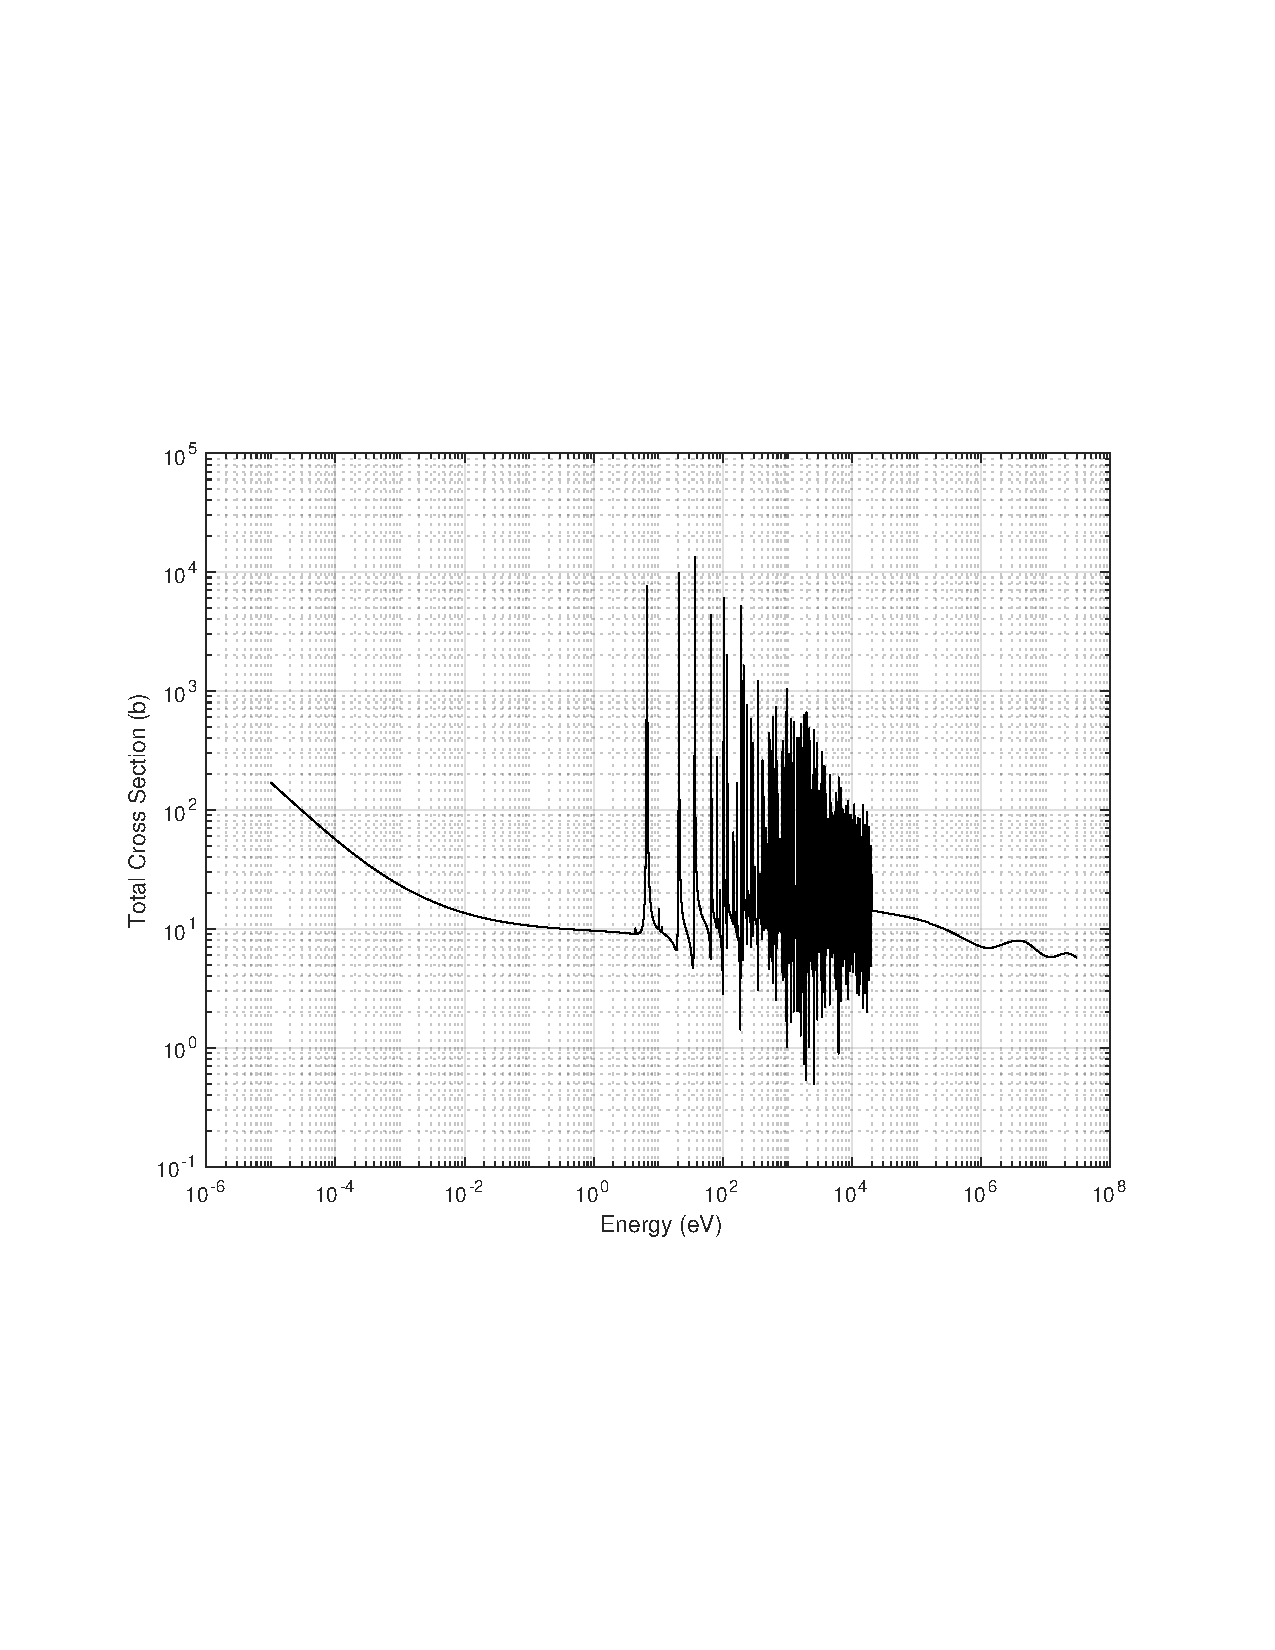
\includegraphics[trim={3.75cm 6.75cm 3.75cm 6.75cm}, width=0.8\textwidth]{./Figures/u238_totalXS_293k.pdf}
\caption{$^{238}$U total cross section at 293~K in ENDF/B-VII.1 processed by NJOY}
\label{Fig:libraryGeneration_u238_totalXS_293K}
\end{center}
\end{figure}

A plot of the $^{238}$U total cross section is given in Fig.~\ref{Fig:libraryGeneration_u238_totalXS_293K} to illustrate these ranges. For this isotope, the thermal range is below a few eV. The resolved resonance range is up until about 20~keV. As we can see, there is much structure. The unresolved resonance range is from 20 to 100~keV. The cross section here appears to be smooth, as only the average or expected cross section is plotted here. In reality, there are resonances that are treated statistically using probability tables, but these are not shown on the plot. The fast region is above 100~keV and is smooth, but contains a few small bumps, primarily because of contributions from higher chance fission.

\subsection{ENDF-6 Format}

If one wants to use nuclear data, they need to be familiar with the ENDF-6 format. Unfortunately, the ENDF format dates back to the 1960s when behemoth computers that were as large as a house that ate punchcards roamed the earth and we have to sadly deal with the cruft that all that legacy entails. Thankfully, it is at least organized and the high level is not all that tricky. As one starts delving into the guts of nuclear data formats, it gets a bit overwhelming. And when one does this long enough, they start speaking an arcane language that sounds like gibberish to the uninitiated listener.

The data formats require specifying the projectile and the target. For the former, we almost always take this as a neutron in reactor physics. For the latter, we need three pieces of information: the charge number $Z$, the mass number $A$, and the isomer state $s$, which is usually the ground state $s = 0$. The charge and mass number are grouped into a single identifier called a ZAID (Z-A ID or more often just pronounced phonetically.) The ZAID is a unique identifier for an isotope given by the following expression:
\begin{align}
  \text{ZAID} = 1000 Z + A .
\end{align}
For example, $^{235}$U is 92235, since $Z = 92$ and $A = 235$.

Once the ZAID is given, we then need to decide which file number within the evaluation to get the data from. This is called the MF number. The most common of these is given in Table~\ref{Table:nuclearData_ENDF_MF}. The most useful of these is MF 3, which stores all of the integral cross sections for every reaction type as a series of points as a function of energy $E$. The MF 2 file contains information about resonance parameters for formulas that are used to create these pointwise cross sections. Information on the differential and double-differential cross sections can be obtained in files 4-6. Of particular note is the fission neutron spectrum $\chi(E)$, which is in MF 5. One odd thing is that the fission multiplicities $\nu$ are in the header, MF 1. Honestly, this feels like a bit of an oversight that got patched in, but as the old saying goes, the less we know about how nuclear data is made the better off we all are.

\begin{table}[htp!]
\caption{Commonly Used ENDF-6 File (MF) Numbers}
\begin{center}
\begin{tabular}{|c|p{12cm}|} \hline
	1	& General Information and Fission Multiplicity Data \\
	2	& Resonance Parameter Information \\
	3	& Cross Sections \\
	4	& Secondary Angular Distributions \\
	5	& Secondary Energy Distributions \\
	6	& Secondary Combined Energy-Angle Distributions \\
	7	& Thermal Scattering Data (see discussion) \\
	8	& Radioactivity and Fission Product Yields \\
	12	& Multiplicities for Photon Production \\
	13	& Cross Sections for Photon Production \\
	14	& Angular Distributions for Photon Production \\
	15	& Energy Distributions for Photon Production \\ \hline
\end{tabular}
\end{center}
\label{Table:nuclearData_ENDF_MF}
\end{table}%

For many of the files, we need to select the reaction type. This is encoded by an MT number. There is little rhyme or reason for how these numbers were handed out, so we just list a few common ones in Table~\eqref{Table:nuclearData_ENDF_MT}.

\begin{table}[htp!]
\caption{Most Relevant ENDF-6 Reaction (MT) Numbers}
\begin{center}
\begin{tabular}{|c|p{12cm}|} \hline
	1	& Total \\
	2	& Elastic Scattering \\
	16	& (n,2n) Multiplicity \\
	18	& Fission \\
	51	& Inelastic Scattering to First Nuclear Level \\
	52	& Inelastic Scattering to Second Nuclear Level \\
	... & \\
	90	& Inelastic Scattering to 40th Nuclear Level \\
	91	& Inelastic Scattering into Continuum \\
	102	& (n,$\gamma$) Radiative Capture \\
	103 & (n,p) Capture \\
	107	& (n,$\alpha$) Capture \\ \hline
\end{tabular}
\end{center}
\label{Table:nuclearData_ENDF_MT}
\end{table}%

Unfortunately, there is a bit of an inconsistency in how thermal scattering law for chemical binding effects is handled. In modern evaluations, these are typically grouped in separate libraries with a file for each particular compound (e.g., hydrogen in light water, carbon in graphite). Typically included are MF types 3 and 7 for the integrated cross section and $S(\alpha,\beta)$ functions. The MT numbers are often a bit arbitrary here. The best strategy here is probably just to look at them all (there are not too many, for better or worse) and just select what we are looking for.

\subsection{JAva-based Nuclear Information Software (JANIS)}

Thankfully, for educational purposes we have easy-to-use tools to access a wide array of the available nuclear data. This means we do not need to concern ourselves with the details of cryptic nuclear data formats. (At least up to the point of doing actual work.) The Nuclear Energy Agency has developed the the JAva-based Nuclear Information Software (JANIS), that supports quick lookups of nuclear data. There are both downloadable and web-based versions available that create both plots as well as tables that can be exported into text files for further processing. Unfortunately, it cannot do everything yet, but is quite powerful and a good way to get oriented or just to do a quick lookup of a cross section. 

The reader is encouraged to play around: \url{https://www.oecd-nea.org/janisweb/}.





%%%%%%%%%%%%%%%%%%%%%%%%%%%%%%%%%%%%%%%%%%%%%%%%%%%%%%%%%%%%%%%%%%%%%%%%%%%%%%%%%%%%%%%%%%%%%%%%%%%%
\section{Point-wise Data Construction}

The ENDF nuclear data files are in formats that are not particularly convenient for use in a reactor analysis. The goal of a nuclear data evaluation is to provide a library that provides a detailed description of the underlying data that accurately describes the physics while keeping storage requirements to a minimum. Because of this, there are a wide number of ways that nuclear data can be represented within ENDF and the evaluator exercises discretion in terms of how this is best done. 

The goal of a nuclear data processing code is to read in the data files and translate it into a usable form. The first step in this process for a cross section is to create a pointwise dataset on an extremely fine grid of energies $E_i$ with corresponding cross section values $\sigma_r^j(E_i)$. In the nomenclature of reactor physics, we often refer to this dataset as a hyperfine library. 

The resolution requirements are defined such that the use of \emph{linear-linear} interpolation will lead to accurate (usually within less than 1\% error) estimation of the cross section over the entire range. The number of datapoints ranges widely depending on the isotope. The simplest isotope, $^1$H can be accurately represented with a few hundred datapoints. On the other extreme, $^{238}$U has a very complicated cross section owing to numerous nuclear resonances, and over $10^5$ energy datapoints are required to accurately represent the cross section. 

Typically the ENDF-6 representation has components spread across two files: File 3 for non-resonance smooth cross sections and File 2 for resonance data and hard-sphere potential scattering. The nuclear data processing code reads both files (if they are present) and produces a cross section that is the sum of the information in these files. We can write the cross section at some energy point $E$ as
\begin{align}
  \sigma(E) = \sigma_\text{smooth}(E) + \sigma_\text{potential}(E) + \sigma_\text{resonance}(E) .
\end{align}
We then take the series of points and assume a linear-linear interpolation to get what is called a pointwise continuous-energy library.

\subsection{Smooth Cross Sections}

A portion of the cross section that is unrelated to the resonances is given in File~3 as point-wise data. Typically, this data are those cross sections that cannot be adequately represented using one of the models for resonance behavior or hard-sphere potential scattering. Most often, this includes the entire unresolved resonance and fast regions as these are above the resonances and a hard-sphere potential model is inadequate to predict the cross section behavior. Depending the evaluation, the rest of the cross section data may or may not be in File 3. In fact, the thermal region can often be reconstructed using resonance parameter data where the ``peak'' occurs at some negative energy value.

\begin{figure}[tb!]
\begin{center}
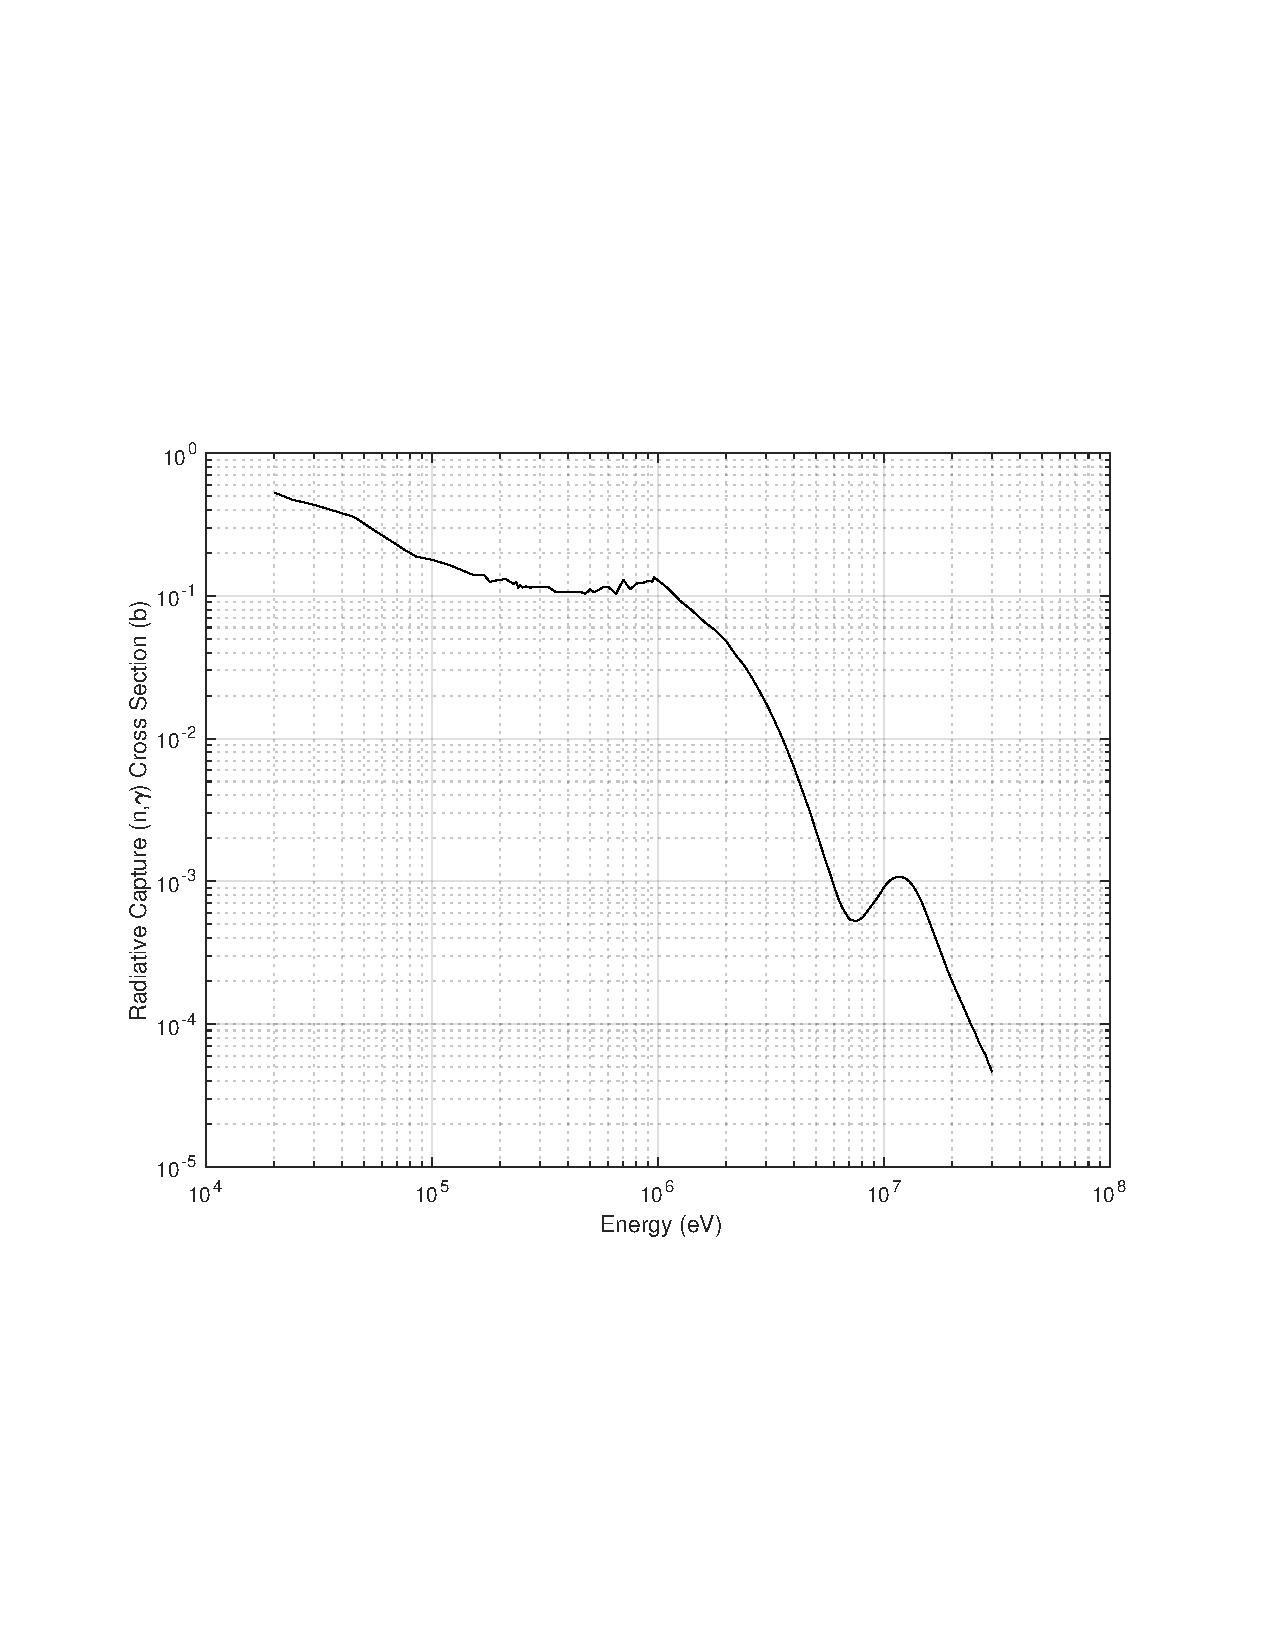
\includegraphics[trim={3.75cm 6.75cm 3.75cm 6.75cm}, width=0.8\textwidth]{./Figures/u238_ngammaXS_mf3.pdf}
\caption{ENDF-6 File 3 $^{238}$U radiative capture (n,$\gamma$) cross section component in ENDF/B-VIII.0}
\label{Fig:libraryGeneration_u238_captureXS_MF3}
\end{center}
\end{figure}

The File 3 contribution of the $^{238}$U radiative capture (n,$\gamma$) cross section is displayed in Fig.~\ref{Fig:libraryGeneration_u238_captureXS_MF3}. Note that this data is zero below 20~keV, which is the boundary between the resolved and unresolved resonance ranges. The information to create the missing data is located in File 2.

\subsection{Hard-Sphere Potential Scattering}

The elastic scattering cross section consists of two components. The first, which is covered in this section, is potential scattering where a neutron scatters off the surface of the nucleus in a billiard-ball like collision. The second part (covered in the next sections) involves the formation of a compound nucleus where a neutron is captured by the nucleus, a neutron is emitted, and the nucleus is left in the ground state.

For low neutron energies, the potential of the nucleus can be approximated as a hard sphere where the neutron wavefunction cannot penetrate into the nucleus. Making this approximation allows for analytical forms for the cross section and provides a compact way to describe this part of the cross section. This information is stored in File 2 of the nuclear dataset.

The fundamental parameter that characterizes potential scattering is the scattering or channel radius $a$, which is proportional to the size of the nucleus. For many nuclei, the channel radius can be approximated by the semi-empirical relationship:
\begin{align}
  a = ( 0.08 + 0.123 A^{1/3} ) \times 10^{-12} \text{ cm}.
\end{align}
Squaring this value gives an area in units of barns. Note that the channel radius can also be given in File 2 as a function of energy $a(E)$ to provide flexibility to accurately describe the scattering cross section.

The incident neutron is characterized by its wave number using the reduced mass of the neutron,
\begin{align}
  k = \frac{ \sqrt{ 2 m_r E }}{ \hbar } = \frac{ \sqrt{ 2 m_n }}{ \hbar }  \left( \frac{A}{A+1} \right) \sqrt{E} ,
\end{align}
where $m_r$ is the reduced neutron mass and $m_n$ is the neutron mass. From this we define a dimensionless parameter as
\begin{align}
  \rho = k a 	\label{Eq:libraryGeneration_rho_ka}
\end{align}
that appears in many of the expressions describing the resonance cross sections.

The incident neutron is described by a plane wave. The nucleus exerts a short-range spherical potential that perturbs the incident neutron wavefunction such that when the outgoing scattered neutron is far from the nucleus, its wavefunction is shifted in phase. This phase shift described by a set of energy-dependent angles $\varphi_\ell(E)$, where $\ell$ denotes the discrete orbital angular momentum values. The potential scattering cross section can be written as a linear combination of the phase shifts from the different angular momenta values as
\begin{align}
  \sigma_p(E) = \sum_{\ell = 0}^\infty ( 2 \ell + 1 ) \frac{4\pi}{k^2} \sin^2 \varphi_\ell .
\end{align}
For energies in the range for which the hard-sphere potential is valid (below a few tens of keV typically) we can describe the cross section with only a few phase shift terms. The four of these are
\begin{subequations}
\begin{align}
  \varphi_0 &= \rho, \\
  \varphi_1 &= \rho - \tan^{-1}\rho , \\
  \varphi_2 &= \rho - \tan^{-1}\left( \frac{3\rho}{ 3 - \rho^2 } \right) , \\  
  \varphi_3 &= \rho - \tan^{-1}\left( \frac{\rho (15 - \rho^2 ) }{ 15 - 6 \rho^2 } \right) .
\end{align}
\end{subequations}
(Note there is a typo on $\varphi_3$ in the 2018 version of the ENDF-6 formats manual.)

An important result is for the low-energy neutron case. In this regime, the $\ell = 0$ term of the potential scattering cross section dominates and $\varphi_0 = \rho$. Furthermore the wave number $k$ is small so $\rho$ is small so we can use the small-angle approximation $\sin\rho \approx \rho$. Therefore,
\begin{align}
  \sigma_p \approx \frac{4\pi}{k^2} \sin^2 \rho \approx \frac{4\pi}{k^2} \rho^2 = \frac{4\pi}{k^2} ( ka )^2 = 4\pi a^2 .
\end{align}
We see that at low energies, the potential scattering cross section converges to a constant value. 

This constant potential scattering approximation is often used in many of the analytical expressions involving resonances and is suitable for low-lying resonances found in isotopes such as $^{238}$U. Note that this cross-sectional area corresponds to the surface area of a spherical nucleus. This may seem weird in the context of a cross-sectional area of sphere, which classically would be $\pi a^2$. This seeming inconsistency is because of the wavelike behavior of the neutron at low energies. The neutron is not a point-like particle at this length scale and as wave, it ``feels'' its way around the entire nucleus and experiences its entire area.

\subsection{Single-Level Breit-Wigner Resonance Model}

The ENDF-6 format allows for resonances to be defined in File 2 using different formats. The most commonly used ones are:
\begin{enumerate}
  \item Single-Level Breit-Wigner,
  \item Multi-Level Breit-Wigner,
  \item Reich-Moore,
  \item R-Matrix Limited.
\end{enumerate}

Of these, the single-level Breit-Wigner form is the most simple, but least accurate, as it is only able to account for a single channel. Most resonances of the major actinides are described using the Reich-Moore formulation. For reasons of pedagogical expediency, we only discuss the single-level Breit-Wigner form and direct interested readers to Appendix D of the ENDF-6 Format Manual for information on the others. 

In the single-level Breit-Wigner format resonances are characterized using a set of parameters:
\begin{align}
  \ell 		&= \text{ orbital angular momentum of the resonance excited state.} \nonumber \\
  I    		&= \text{ spin (angular momentum) of the target nucleus.} \nonumber \\
  J			&= \text{ spin state of the resonance for the compound nucleus.} \nonumber \\
  g_J		&= (2J + 1)/[2(2I+1)] = \text{ statistical spin factor.} \nonumber \\
  E_r		&= \text{ peak energy of the $r$th resonance.} \nonumber \\
  \Gamma_{nr}(|E_r|) &= \text{ neutron (elastic scattering) line width for the $r$th resonance at energy $E_r$.} \nonumber \\
  \Gamma_{\gamma r}  &= \text{ radiative capture (n,$\gamma$) line width for the $r$th resonance.} \nonumber \\
  \Gamma_{fr} 		 &= \text{ fission (n,f) line width for the $r$th resonance.} \nonumber \\
  \Gamma_r(|E_r|)	 &= \Gamma_{nr}(|E_r|) + \Gamma_{\gamma r} + \Gamma_{fr} = \text{ total line width for $r$th resonance.} \nonumber
\end{align} 

The neutron line width is a function of energy, whereas the radiative capture and fission are not. The file gives the resonance width at \emph{absolute value} of the resonance peak energy $E_r$. This is important because there can be negative energy resonances, which correspond to bound states within the compound nucleus that are classically inaccessible because even a neutron with zero kinetic energy forming that compound nucleus would put it into an excited state with an energy above those states. While these states are classically inaccessible, the fact that the energy state is indeterminate from quantum mechanics means there is still a contribution to the cross section at positive energies from these bound state resonances.

The energy-dependence of the neutron line width is because the neutron penetrates a certain depth into the nucleus and the amount of penetration is a function of kinetic energy and the orbital angular momentum state of the resonance. This is
\begin{align}
  \Gamma_{nr}(E) = \frac{\Pi_\ell(E)}{\Pi_\ell(|E_r|)} \Gamma_{nr}(|E_r|) .
\end{align}
Here $\Pi_\ell$ are the penetrability factors, which are
\begin{subequations}
\begin{align}
  \Pi_0 &= \rho, \\
  \Pi_1 &= \frac{\rho^3}{1 + \rho^2}, \\
  \Pi_2 &= \frac{\rho^5}{9 + 3\rho^2 + \rho^4}, \\  
  \Pi_3 &= \frac{\rho^7}{225 + 45\rho^2 + 6\rho^4 + \rho^6}.
\end{align}
\end{subequations}
Here $\rho$ is given by Eq.~\eqref{Eq:libraryGeneration_rho_ka}, which depends on energy by way of the wavenumber. Note that the penetrability factors are more often described with the variable $P_\ell$, but we change this here so as not to confuse them with the Legendre polynomials.

For angular momenta $\ell > 0$, the effective peak of the resonance is given by $E_r'$, which is itself a function of energy by way of the shift factors $S_\ell$. This is
\begin{align}
  E_r'(E) = E_r + \frac{ S_\ell(|E_r|) - S_\ell(E) }{ 2 \Pi_\ell(|E_r|) } \Gamma_{nr}(|E_r|).
\end{align}
The shift factors are
\begin{subequations}
\begin{align}
  S_0 &= 0, \\
  S_1 &= -\frac{1}{1 + \rho^2}, \\
  S_2 &= -\frac{18 + 3\rho^2}{9 + 3\rho^2 + \rho^4}, \\  
  S_3 &= -\frac{675 + 90 \rho^2 + 6 \rho^4 }{225 + 45\rho^2 + 6\rho^4 + \rho^6}.
\end{align}
\end{subequations}

We can now proceed with giving the resonance cross section formulas. These are taken for a target at rest or zero temperature. Normally these would then be adjusted for the actual temperature in a process called Doppler broadening that we discuss in the next section.

The absorption (with radiative capture and fission being the most relevant) resonances are simpler than scattering, so we discuss these first. The contribution from the resonances for these reactions are
\begin{align}
  \sigma_x(E) = \frac{4\pi}{k^2} \sum_{\ell = 0}^L \sum_J g_J \sum_{r = 1}^{N_J} \frac{ \Gamma_{nr} \Gamma_{xr} }{ 4 ( E - E_r' )^2 + \Gamma_r^2 } , \quad x \in \gamma, f.
\end{align} 
The energy dependencies of the quantities $\Gamma_{nr}$ $\Gamma_r$, and $E_r'$ are omitted for brevity. In ENDF-6 File 2, the resonances are given as pairs of $\ell$ and $J$ values, so effectively we end up summing over all resonances in the file and using the appropriate definitions.

The elastic scattering resonance cross section includes two terms. The first is similar to that of absorption and accounts for compound nucleus formation. The second term is because of interference between compound nucleus formation and potential scattering. This arises because each event has an associated wavefunction that must be squared (multiplied by complex conjugate) to get the cross section and the interference term is the cross term from that operation. The resulting expression for the resonance cross sections are
\begin{align}
  \sigma_s(E) = \frac{4\pi}{k^2} \sum_{\ell = 0}^L \sum_J g_J \sum_{r = 1}^{N_J} \frac{ \Gamma_{nr}^2 - 2 \Gamma_r \Gamma_{nr} \sin^2\varphi_\ell + 2 (E - E_r' ) \Gamma_{nr} \sin(2\varphi_\ell) }{ 4 ( E - E_r' )^2 + \Gamma_r^2 } .
\end{align} 
Note again that the energy dependencies of the quantities $\Gamma_{nr}$ $\Gamma_r$, $\varphi_\ell$, and $E_r'$ are omitted.

The resonance contribution to the total cross section is the sum of the radiative capture, fission, and elastic scattering components.

\subsection{Pointwise Construction Algorithm}

The task is to construct an approximate pointwise representation of the continuous-energy cross section subject to interpolation schemes between the energy grid points. For neutron cross sections, we typically use linear-linear interpolation between the energy $E$ and the cross section $\sigma(E)$. Given a set of energies $E_i$ and cross sections $\sigma(E_i) = \sigma_i$, we have an approximate interpolated cross section of
\begin{align}
  \widetilde{\sigma}(E) = \sigma_i + \frac{ E - E_i }{ E_{i+1} - E_i } ( \sigma_{i+1} - \sigma_i ) .
\end{align}

Other interpolation schemes are possible. For example, photon libraries use typically logarithmic interpolation schemes, which are to be more appropriate for photons given the energy dependence of the cross sections. Going back to neutrons, one might be tempted to use higher-order polynomials to approximate the cross section such as cubic splines. Usually this is not done because it would complicate the interpolation. For cubic splines this would involve some numerical root finding scheme every time a cross section needs to be interpolated, which would drive up the expense of many downstream calculations. Second, the functional form of resonances means that while we would reduce the number of points going to higher-order polynomials, it would not actually save us all that much to justify the downstream burdens. Therefore, this motivates us to stick with piecewise linear cross sections.

To find an appropriate energy grid, we need to select a set of points that meets some global error tolerance $\epsilon$ such that the relative error in the interpolated cross section versus the actual cross section is less than epsilon,
\begin{align}
  \frac{ | \widetilde{\sigma}(E) - \sigma(E) | }{ \sigma(E) } \le \epsilon ,
\end{align}
for all energies $E$. Guaranteeing this for every energy is very difficult, so we often relax this using a method of bisection.

The first step in the bisection method is to start with a set of essential energy points. These essential points usually include:
\begin{enumerate}
  \item The energy points specified in the smooth cross section in File 3,
  \item The resonance peaks $E_r$ specified in file 2,
  \item Reaction thresholds for inelastic scattering or other threshold reactions,
  \item The minimum, maximum, energy group boundary points, and any others specified by the end user.
\end{enumerate}
The reason for the File 3 points is these were already chosen by the nuclear data evaluator to be the best set of points to most efficiently describe the cross section and removing them may introduce additional errors. The resonance peak energies $E_r$ represent places where the cross section experiences a sharp changes and excluding these points could mean that the algorithm could miss an entire resonance, which would lead to major errors in a downstream calculation. The third set is essential to ensure we preserve reaction thresholds lest we could have unphysical behavior. For the fourth, these represent points the user explicitly wants to have an accurate cross section or should exist in the library for the purpose of convenience, such as energy group boundaries.

We now proceed to loop over the energy grid points. Suppose we are at energy grid point $i$, we compute the midpoint energy $E_{mid} = (E_i + E_{i+1} )/2$ and then compute the exact cross section at $E_{mid}$ and the approximation using linear-linear interpolation. If these values are \emph{not} within a relative error tolerance $\epsilon$, we add $E_{mid}$ to the energy grid and reindex the energy grid points such that $E_{i+1} \rightarrow E_{mid}, E_{i+2} \rightarrow E_i$, and so on. We then repeat the process, computing a new value of $E_{mid}$, evaluating the cross sections and inserting points as needed until we achieve a fine enough resolution to meet the error tolerance, at which point we move onto the next energy grid point and bisect for that range. This process continues until we reach the end of the energy grid structure.

This discussion assumes we do this for every cross section independently. This leads to the complication of having different energy grids for every reaction cross section and every isotope. One extreme is to use a unionized energy grid for every isotope and every reaction. This leads to exceptionally large files and is usually not done. The usual compromise is to use the same energy grid for all reactions of the same isotopes with different energy grids for different isotopes. (The exception here is threshold reactions, which are zero below a certain energy and these zeros are usually not stored explicitly.)

This modifies the algorithm slightly in that we do the bisection simultaneously for all reactions within an isotope and we test that all the cross sections for all reactions are within the relative error tolerance. If any one of them fails, we add another point to the grid.

The final point here relates to the total cross section or any others that are the sum of a series of partials (e.g., absorption or inelastic). Usually it is best to perfrom the pointwise construction on all of the individual reaction cross sections. All combined cross sections such as the total cross section are then computed as the sum of the partials. In this manner, we guarantee that the cross sections add together correctly.

%%%%%%%%%%%%%%%%%%%%%%%%%%%%%%%%%%%%%%%%%%%%%%%%%%%%%%%%%%%%%%%%%%%%%%%%%%%%%%%%%%%%%%%%%%%%%%%%%%%%
\section{Doppler Broadening}

The smooth cross sections from File 3 and those constructed from resonance parameters given in File 2 are taken to be for a target at rest or zero temperature. Of course, any actual system will be at a finite temperature and this has a major effect on the microscopic cross sections. The reason is that the background nuclei experience random thermal motion and therefore the neutrons encounter these nuclei at different relative velocities or energies. The cross section of any individual interaction is taken at this relative energy. Since we cannot know the precise velocity of the target nuclei in every collision, we need to average over all possible nuclear velocities in a process called thermal averaging or more often Doppler broadening.

The most pronounced impact on the cross sections occur near the resonances. Recall the cross section near a resonance is a highly peaked function and the effect of Doppler broadening is to smooth this peak out, broadening the resonance. The higher the temperature, the more broadening that occurs. This means that the resonance impacts a large range of energies and neutrons are more likely to interact with the resonance. In light-water reactors with low-enriched uranium fuel, the Doppler broadening of the $^{238}$U resonances leads to a significant increase in the amount of absorption from them. This Doppler effect is one of the most important physical mechanisms that need to get resolved correctly to get the right reaction rates and therefore criticality.

\subsection{Maxwell-Boltzmann Distribution}

The velocities of particles in thermodynamic equilibrium are described by a Maxwell-Boltzmann distribution. The velocity in each independent direction $(V_x,V_y,V_z)$ is described by a normal distribution. The distribution for the speed can then be written as
\begin{align}
  M(\mathbf{V},T) dV_x dV_y dV_z 
  = \left( \frac{ A m_n }{ 2 \pi k_B T } \right)^{3/2} \exp \left( -\frac{ A m_n V^2 }{ 2 k_B T } \right) dV_x dV_y dV_z
\end{align}
where the speed is
\begin{align}
  V = \sqrt{ V_x^2 + V_y^2 + V_z^2 } .
\end{align}
This can expressed in spherical coordinates in terms of the speed $V$ as
\begin{align}
  M(V,\mu,\gamma,T) dV d\mu d\gamma &= \frac{1}{4\pi} M(V,T) dV d\mu d\gamma \nonumber \\
  &= \left( \frac{Am_n}{2\pi k_B T} \right)^{3/2} \exp \left( -\frac{ A m_n V^2 }{ 2 k_B T } \right) V^2 dV d\mu d\gamma.
\end{align}
Here $V^2 dV d\mu d\gamma$ is a 3-D differential velocity element analogous to a differential volume element. Here $\mu$ is the cosine of the angle between the nucleus an arbitrary polar axis, which is usually chosen as the incident neutron direction, and $\gamma$ is the azimuthal angle about that axis.

We then define
\begin{align}
  \beta = \frac{A m_n}{ 2 k_B T },
\end{align}
giving
\begin{align}
  M(V,\mu,\gamma,T) dV d\mu d\gamma = \left( \frac{\beta}{\pi} \right)^{3/2} e^{-\beta V^2} V^2 dV d\mu d\gamma.
\end{align}

From here we can work out the integrals and show that this distribution is normalized such that
\begin{align}
  \int_0^{2\pi} \int_{-1}^1 \int_0^\infty  M(V,\mu,\gamma,T) dV d\mu d\gamma = \int_0^\infty M(V,T) dV = 1.
\end{align}
This normalization will become important to conserve particles in collisions.

This distribution can be transformed to be in terms of the kinetic energy of the nucleus. Performing the variable transformation,
\begin{align}
  E &= \frac{1}{2} A m_n V^2, \nonumber \\
  dE &= A m_n V dV . \nonumber
\end{align}
and integrating out the $\mu$ and $\gamma$ variables gives
\begin{align}
  M(E,T) dE 
  = &\frac{2}{\sqrt{\pi} k_B T} \sqrt{ \frac{A E}{k_B T} } \exp \left( -\frac{ AE }{ k_B T } \right) dE.
\end{align}

We assume that the velocities of the background nuclei are distributed approximately with the Maxwell-Boltzmann distribution. In reality, in a solid, for example, the velocities in some directions could be inhibited by chemical bonds. Fortunately, for temperatures that are not too low, those well in excess of the Debye temperature, the assumption is a very good one. This applies for most materials we encounter in reactor analysis for room temperature and above.

\subsection{Thermal Averaging of Cross Sections}

If we average over all possible nuclear velocities for a media with temperature $T$, we get a reaction rate per incident neutron with speed $v$ of
\begin{align}
  R(v) = v \sigma(v,T) = \int_0^{2\pi} \int_{-1}^1 \int_0^\infty v_{rel} \sigma(v_{rel},0) M(V,T) dV d\mu d\gamma . 
\end{align}
Here we suppressed the reaction-type index on the cross section. The variable $v_{rel}$ is the relative speed between the incident neutron and the target nucleus. Using the law of cosines, we can write the relative speed as
\begin{align}
  v_{rel} = \sqrt{ v^2 + V^2 - 2 v V \mu } .
\end{align}
Since this is independent of the azimuthal angle $\gamma$ and nothing else in the integral is as well, we can simply carry out that integration to get
\begin{align}
  R(v) = v \sigma(v,T) = \frac{1}{2} \int_{-1}^1 \int_0^\infty v_{rel} \sigma(v_{rel},0) M(V,T) dV d\mu  . \label{Eq:libraryGeneration_thermalAverageReactionRate_azimuthallyIntegrated}
\end{align}

The presence of $\mu$ in the $v_{rel}$ and therefore the zero-temperature cross section $\sigma(v_{rel},0)$ is problematic from doing this integral. It turns out that the problem is easier if instead we integrate over the relative speed using a variable transformation between $\mu$ and $v_{rel}$. By differentiating the relative speed with respect to $\mu$ we obtain
\begin{align}
  d\mu = -\frac{v_{rel}}{v V} dv_{rel} .
\end{align}

The limits of integration are a bit tricky to work out. First, $\mu$ has the range $[-1,1]$, but it is under a square root, so we must be careful. Second, the minus sign from the transformation flips the limits of integration. 

The $\mu = -1$ case (upper limit after the flip) is straightforward, giving $v_{rel} = \sqrt{(v+V)^2} = V + v$, discarding the nonphysical negative sign. This gives the range $v_{rel} < V + v$.

\begin{figure}[tb!]
\begin{center}
\begin{center}
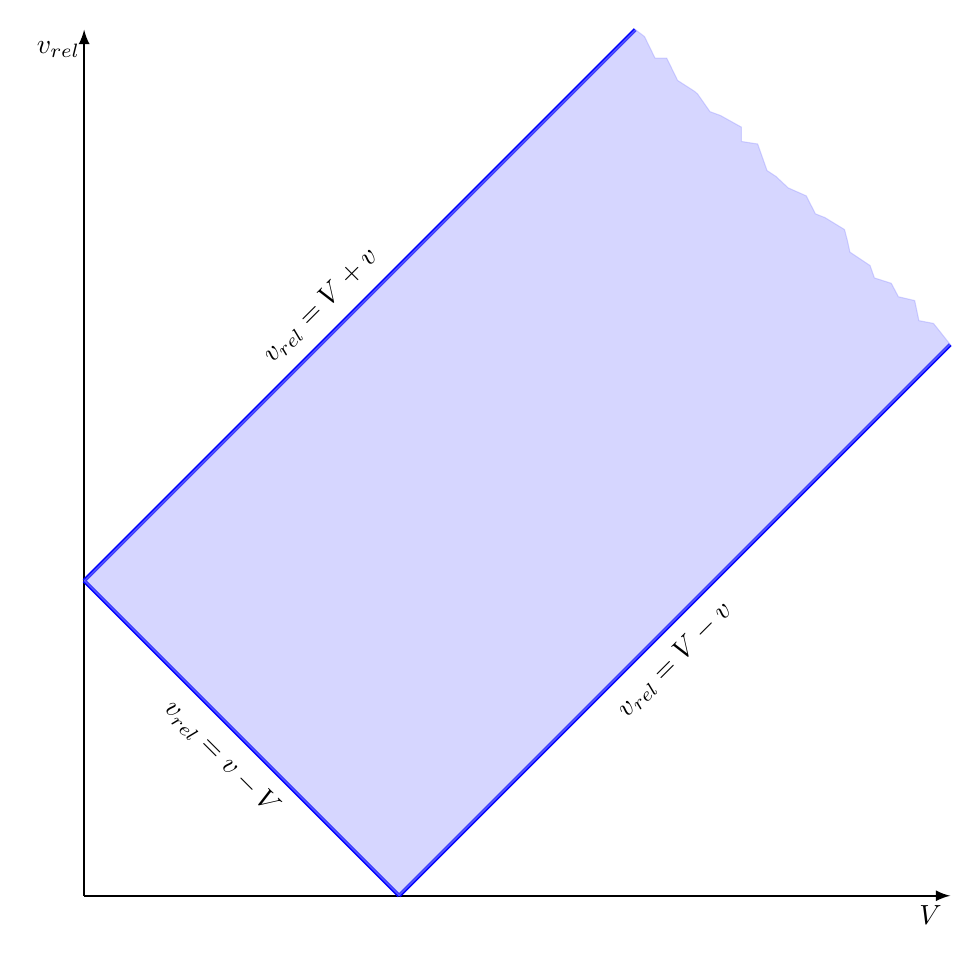
\begin{tikzpicture}
  \draw[-latex,thick] (0,0) -- (0,11);
  \draw[-latex,thick] (0,0) -- (11,0);
  \node at (10.75,-0.25) {$V$};
  \node at (-0.325,10.75) {$v_{rel}$};
  
  \draw[line width=0.5mm,blue] (0,4) -- (7,11);
  \draw[line width=0.5mm,blue] (4,0) -- (11,7);
  \draw[line width=0.5mm,blue] (0,4) -- (4,0);
  
  \filldraw[blue!40, opacity=0.4, decoration={random steps,segment length=0.2cm}] (4,0) -- (0,4) -- (7,11) decorate{-- (11,7)} -- cycle;
  
  \node[rotate =  45] at (7.5,3) {$v_{rel} = V - v$};
  \node[rotate =  45] at (3,7.5) {$v_{rel} = V + v$};
  \node[rotate = -45] at (1.75,1.75) {$v_{rel} = v - V$};
\end{tikzpicture}
\end{center}
\caption{Integration range for thermally averaged reaction rate}
\label{Fig:libraryGeneration_thermalAveragingIntegrationRange}
\end{center}
\end{figure}

The case of $\mu = 1$ (lower limit after the flip) yields $v_{rel} = \sqrt{(v - V)^2} = \pm ( v - V )$. There are two potentially physically meaningful solutions: $v - V$ when $v > V$ and $V - v$ when $v < V$. This implies the respective ranges of $v_{rel} > v - V$ and $v_{rel} > V - v$. Taking the intersection of these three ranges yields the integration range depicted in Fig.~\ref{Fig:libraryGeneration_thermalAveragingIntegrationRange}.

These integration ranges can be written compactly using the absolute value
\begin{align}
  R(v) = v \sigma(v,T) = \frac{1}{2 v} \int_0^\infty v_{rel}^2 \sigma(v_{rel},0) \int_{|v-v_{rel}|}^{|v+v_{rel}|} \frac{1}{V} M(V,T) dV dv_{rel}  .
\end{align}
We can then carry out the inner integral over the target speed $V$. The result in terms of the incident neutron speed $v$ and relative speed between it and the target nucleus $v_{rel}$ is then
\begin{align}
  R(v) = v \sigma(v,T) = \frac{1}{v} \sqrt{ \frac{\beta}{\pi} } \int_0^\infty v_{rel}^2 \sigma(v_{rel},0) \left[ e^{-\beta ( v - v_{rel} )^2} -  e^{-\beta ( v + v_{rel} )^2} \right] dv_{rel}  .
\end{align}

We can then cast this to be in terms of the neutron energy. We define the relative kinetic energy experienced by the target nucleus as
\begin{align}
  E_{rel} = \frac{1}{2} m_n v_{rel}^2 . \nonumber
\end{align}
We then obtain the thermally averaged cross section as
\begin{align}
   \sigma(E,T) &= \frac{1}{2 E} \sqrt{ \frac{\alpha}{\pi} } \int_0^\infty \sqrt{E_{rel}} \sigma(E_{rel},0) \nonumber \\ &\times \left[ \exp\left( -\alpha \left( \sqrt{E} - \sqrt{E_{rel}} \right)^2 \right) -  \exp\left( -\alpha \left( \sqrt{E} + \sqrt{E_{rel}} \right)^2 \right) \right] dE_{rel}  \label{Eq:libraryGeneration_thermalAveragedXS_energy}
\end{align}
where
\begin{align}
  \alpha = \frac{A}{k_B T} .
\end{align}
(This $\alpha$ is different than the scattering ratio.)

From here we need to know the functional form of the cross section. There are two cases that appear commonly and can actually be worked out analytically. 

The first is the case of a $1/v$ absorber. To solve this, it is actually easier to use Eq.~\eqref{Eq:libraryGeneration_thermalAverageReactionRate_azimuthallyIntegrated} directly:
\begin{align}
  \sigma(v,T) = \frac{1}{2v} \int_{-1}^1 \int_0^\infty v_{rel} \left( \frac{1}{v_{rel}} \right)  M(V,T) dV d\mu  = \frac{1}{v}  \int_0^\infty  M(V,T) dV = \frac{1}{v} .
\end{align}
Here we recall that the Maxwell-Boltzmann distribution $M(V,T)$ is normalized such that integrating over all target speeds yields one. This result says that a $1/v$ cross section is unaffected by thermal motion.

The second case is constant (hard-sphere) potential scattering $\sigma(v_{rel},0) = \sigma_p$. For this we can work out the integral of the final result directly to obtain
\begin{align}
  \sigma(E,T) = \sigma_p \left[  \left( 1 + \frac{ k_B T }{ 2 A E } \right) \erf \left( \sqrt{\frac{AE}{k_B T}} \right) + \sqrt{ \frac{ k_B T }{ \pi A E } } \exp \left( -\frac{AE}{k_B T} \right) \right]. \label{Eq:libraryGeneration_FreeGasScatteringXS}
\end{align}
We see that the potential scattering cross section gets corrected by an energy-dependent factor involving familiar exponentials and perhaps a less familiar function called the \emph{error function}. The error function was first studied in the domain of statistical inference, which led to its name. Unfortunately, even through neutron interactions have little to do with the topic, we are stuck with the name. The error function is defined by the following integral:
\begin{align}
   \text{erf}(x) = \frac{2}{\sqrt{\pi}} \int_0^x e^{-t^2}  dt .
\end{align}
This is available in any standard mathematics library.

The above expression is not particularly intuitive, but the limiting behavior for low and high energies is insightful. At low energies, the error function goes to zero and its factor diverges. Using L'Hopital's rule, we can show that this term limits to a constant value. The second term, on the other hand, diverges because the exponential tends toward one while the $1/\sqrt{E}$ factor diverges. Because this is equivalent to inverse speed and the constant becomes small for small speed $v$, we can assert that:
\begin{subequations}
\begin{align}
  \sigma_s(E,T) = \sqrt{ \frac{ k_B T }{ \pi A }  } \frac{\sigma_p}{v}, \quad E \ll k_B T.
\end{align}
The behavior of the scattering cross at low energies exhibits the same trend as capture cross sections.

At high energies, the both the error function term and its factor converges to one. The exponential term tends toward zero. Therefore, for high energies, we can state
\begin{align}
  \sigma_s(E,T) = \sigma_s(E) = \sigma_p, \quad E \gg k_B T .
\end{align}
\end{subequations}
It is often acceptable to make this assumption in the resonance region, which simplifies the analysis in reactor physics calculations.

It is also possible to develop approximate, semi-analytical expressions for the single-level Breit-Wigner form of the cross section for $\ell = 0$ resonances in terms of the $\psi$ and $\chi$ functions called the \emph{Bethe-Placzek cross sections}. Because these expressions are quite limited in their applicability, we will not go through the entire derivation, which is given in many other reactor physics texts (see Bell \& Glasstone). Nonetheless, they are still useful because they can serve as a check on the more general method for Doppler broadening discussed in the next section.

The Bethe-Placzek absorption cross section for a single resonance $r$ is
\begin{align}
  \sigma_{zr}(E,T) = \sigma_0 \frac{\Gamma_{zr}}{\Gamma_r} \sqrt{ \frac{E_0}{E} } \psi(\zeta,x) , \quad z \in \gamma,f
\end{align}
where the $\psi$ function is
\begin{align}
  \psi(\zeta,x) = \frac{\zeta}{2\sqrt{\pi}} \int_{-\infty}^\infty \frac{1}{1+y^2} \exp \left( -\frac{\zeta^2}{4} ( x - y )^2 \right) dy , \label{Eq:nuclearData_DopplerBroadening_psi}
\end{align}
and the quantity $\sigma_0$ is a cross section given by
\begin{align}
  \sigma_0 = 4\pi \lambdabar_0 g_J \frac{ \Gamma_{nr}(|E_r|) }{ \Gamma_r(|E_r|) } ,
\end{align}
with dimensionless energy
\begin{align}
  x = \frac{2}{\Gamma_r(|E_r|)} ( E - E_r )
\end{align}
and $\lambdabar_0$ being the reduced wavelength of a neutron with a speed corresponding to energy $E_r$,
\begin{align}
  \lambdabar_0 = \frac{A+1}{A} \frac{\hbar}{ m_n v(|E_r|) }  .
\end{align} 
The $\psi$ function needs to be evaluated using numerical integration.

The corresponding Bethe-Placzek scattering cross section is
\begin{align}
  \sigma_s(E,T) = \sigma_p + \sigma_0 \frac{\Gamma_n}{\Gamma} \psi(\zeta,x) + \sigma_0 \frac{a}{\lambdabar} \chi(\zeta,x) ,
\end{align}
where this new function $\chi(\zeta,x)$ can be found using numerical integration:
\begin{align}
  \chi(\zeta,x) = \frac{\zeta}{\sqrt{\pi}} \int_{-\infty}^\infty \frac{y}{1+y^2} \exp \left( -\frac{\zeta^2}{4} ( x - y )^2 \right) dy
\end{align}

\subsection{Doppler Broadening of Piecewise-Linear Cross Sections}

A cross section library is typically represented using a piecewise-linear representation with a resolution chosen to accurately represent the underlying cross section's energy dependence. The goal is to perform Doppler broadening given this piecewise-linear representation at zero temperature as input where the output is another piecewise-linear representation of the Doppler broadened cross section. This can be done exactly using a method often called SIGMA1, which is named after the original code developed by Cullen in the 1970s.

We begin with Eq.~\eqref{Eq:libraryGeneration_thermalAveragedXS_energy} and introduce the following transformation variables:
\begin{subequations}
\begin{align}
  y^2 &= \beta v^2 = \alpha E \\*
  x^2 &= \beta v_{rel}^2 = \alpha E_{rel} .
\end{align}
\end{subequations}
Inserting these gives
\begin{align}
  \sigma(y,T) &= \frac{1}{y^2 \sqrt{\pi}} \int_0^\infty x^2 \sigma(x,0) \left[ e^{-(x-y)^2} - e^{-(x+y)^2} \right] dx.
\end{align}
We define the function
\begin{align}
  \eta(y,T) &= \frac{1}{y^2 \sqrt{\pi}} \int_0^\infty x^2 \sigma(x,0) e^{-(x-y)^2} dx,
\end{align}
which implies the Doppler broadened cross section can be expressed as
\begin{align}
  \sigma(y,T) = \eta(y,T) - \eta(-y,T) .
\end{align}

The cross section is given as a piecewise linear function in energy with cross sections given at grid points $k$ of $\sigma_k$ at energy $E_k$ and $\sigma_{k+1}$ at energy $E_{k+1}$. Transforming into $x$, we can write the cross section as a quadratic function,
\begin{align}
  \sigma(x,0) = A_k + C_k x^2, \quad x \in [x_k,x_{k+1}) .
\end{align}
where $C_k$ is the slope
\begin{align}
  C_k = \frac{ \sigma_{k+1} - \sigma_k }{ x_{k+1}^2 - x_k^2 } \nonumber
\end{align}
and $A_k$ is the intercept that can be found by solving
\begin{align}
  A_k = \sigma_k - C_k x_k^2 . \nonumber
\end{align}

We then insert the piecewise-linear form of the cross section into the expression for $\eta$ to get
\begin{align}
  \eta(y,T) &= \frac{1}{y^2 \sqrt{\pi}} \sum_k \int_{x_k}^{x_{k+1}} x^2 \left( A_k + C_k x^2 \right) e^{-(x-y)^2} dx ,
\end{align}
We then introduce the transformation
\begin{align}
  z = x-y \nonumber
\end{align}
to obtain
\begin{align}
  \eta(y,T) 
  &= \frac{1}{y^2 \sqrt{\pi}} \sum_k \int_{x_k-y}^{x_{k+1}-y} (z+y)^2 \left( A_k + C_k (z+y)^2 \right) e^{-z^2} dz \nonumber \\
  &= \frac{1}{y^2 \sqrt{\pi}} \sum_k \int_{x_k-y}^{x_{k+1}-y} ( z^2 + 2zy + y^2 ) \left[ A_k + C_k ( z^2 + 2zy + y^2 ) \right] e^{-z^2} dz \nonumber \\
  &= \frac{1}{y^2 \sqrt{\pi}} \sum_k \int_{x_k-y}^{x_{k+1}-y} \bigg[ C_k z^4 + 4 C_k y z^3 + ( A_k + 6 C_k y^2 ) z^2  \nonumber \\
  &\hspace{2.5cm}  + ( 2 A_k y + 4 C_k y^3 ) z + ( A_k y^2 + C_k y^4 )  \bigg] e^{-z^2} dz
\end{align}

This expression can be evaluated analytically by defining
\begin{subequations}
\begin{align}
  F_n(a)   &= \frac{2}{\sqrt{\pi}} \int_0^a z^n e^{-z^2} dz , \\
  H_n(a,b) &= F_n(b) - F_n(a) .
\end{align}
\end{subequations}
The $F_n$ functions can be carried out analytically as
\begin{subequations}
\begin{align}
  F_0(a) &= \erf(a) , \\
  F_1(a) &= \frac{1}{\sqrt{\pi}} \left( 1 - e^{-a^2} \right), \\
  F_2(a) &= \frac{1}{2} \erf(a) - \frac{a}{\sqrt{\pi}} e^{-a^2} , \\
  F_3(a) &= \frac{1}{\sqrt{\pi}} \left[ 1 - ( 1 + a^2 ) e^{-a^2} \right] , \\
  F_4(a) &= \frac{3}{4} \erf(a) - \frac{1}{\sqrt{\pi}} \left( a^3 + \frac{3a}{2} \right) e^{-a^2} .
\end{align}
\end{subequations}


The algorithm can be generalized to broaden any library from temperature $T_1$ to a \emph{higher} temperature $T_2$. The only changes in the algorithm replaces $\sigma(x,0)$ with $\sigma(x,T_1)$ in the integrand and the temperatures in the parameters $\beta$ and $\alpha$ become $\Delta T = T_2 - T_1$.

There are a few practical considerations. The first is that the integration limits are from zero to infinity. A piecewise linear cross section set usually does not extend to zero (as the cross section becomes infinite) and certainly must end before becoming infinite. The question then is what to do here. One option is to simply ignore the integral outside the range. This can work if the range is wide enough to limit the truncation errors. Another option is to extrapolate. A common approach is to assume a linear extrapolation down to zero energy based on the slope of the first energy range and to assume the cross section for energies that the upper limit is equal to the cross section at the top of the energy range.

The second practical implementation point relates to the fact that the algorithm is effectively a double-nested loop over the entire cross section library. The $^{238}$U library includes over $10^5$ points, meaning there would be over $10^{10}$ calculations to execute the routine exactly. In reality, the exponentials fall off rather quickly and we can truncate them with minimal loss of accuracy. A conventional range of significance for the $\eta(y,T)$ in terms of the relative velocity is 
\begin{align}
  v - \frac{4}{\sqrt{\beta}} \le v_{rel} \le v + \frac{4}{\sqrt{\beta}} . \nonumber
\end{align}
Since $v = y/\sqrt{\beta}$ and $v_{rel} = x/\sqrt{\beta}$, we can deduce a range of significance of
\begin{align}
  y - 4 \le x \le y + 4. \nonumber
\end{align}
For the $\eta(-y,T)$ term, we have
\begin{align}
  0 \le x \le 4 - y. \nonumber
\end{align}
The integration range should, at a minimum, include contributions from all points satisfying these ranges.

Another issue comes from evaluating the functions $H_n(a,b)$ using a direct difference formula $F_n(b) - F_n(a)$ with finite precision arithmetic. When these $F_n$ are about equal in magnitude, there can be a loss of precision leading to a significant accumulation of error. The general strategy is when $F_n(b) - F_n(a) < \epsilon$, a Taylor series expansion of $F(b)$ about $b = a$ is performed. Therefore, we have
\begin{align}
  H(a,b) = \sum_{m=1}^\infty \frac{(b-a)^m}{m!} F_n^{(m)}(a) .
\end{align}
Here the $(m)$ superscript denotes the $m$th derivative. The summation is terminated when the contributions become small enough to be neglected.

Another problem that can arise when Doppler broadening relates to not having enough resolution in the broadened cross section. In the zero-temperature library, numerous points are needed about the peak of the resonance and relatively few on the wings. When the cross section is broadened, the resonance spreads out and we end up in a scenario where there is an excessive number of points near the peak and too few in the area where the resonance falls off. The former is not a problem in accuracy, only efficiency. The latter, however, can lead to significant errors in the cross section representation. A production-level code addresses this by implementing an adaptive coarsening and refining algorithm to ensure the broadened cross section library has an appropriate resolution.





%%%%%%%%%%%%%%%%%%%%%%%%%%%%%%%%%%%%%%%%%%%%%%%%%%%%%%%%%%%%%%%%%%%%%%%%%%%%%%%%%%%%%%%%%%%%%%%%%%%%
\section{Multigroup and $P_N$ Approximations}

The continuous energy library results in a dataset containing over $10^5$ points, which is simply too large for routine design calculations. We need to somehow reduce this dimensionality while still preserving accuracy. This is done through the multigroup approximation. In this approximation, we select an energy group structure that allows for a designer to accurately describe the important characteristics of the reactor. Once this is chosen, we then integrate the transport equation over each energy group to form a system of coupled equations with one equation per energy group. This integration process involves some inherent approximations that we discuss here.

Once we have the system of equations, we then are faced with the problem of calculating the representative coefficients or group cross sections. Determining these presents a difficult challenge in reactor analysis that to this day still remains unaddressed. The remainder of this chapter is devoted to this topic specifically.

\subsection{Energy Group Structure}

The first task we need to handle is to define an energy group structure or energy discretization. Unfortunately, this choice depends on the system being analyzed and is largely a matter of intuition, experience, and trial and error. For the purposes here, we will assume that we are given the energy group structure for a particular application. 

That said, we should discuss the considerations and the tradeoffs. First, a good choice of group structure covers relevant energy ranges of physics with significant effect. The obvious choice is having fast versus thermal neutron groups because neutrons behave qualitatively differently in these energy ranges. Additional considerations arise from the resonance structure, where we often separate the fast region into the resonance and continuum regions and usually give important resonances their own energy groups. A general strategy is to select resonance groups such that each important resonance is roughly at the center of the group. 

Given that we make choices that delineate different physics, we note the tradeoffs between using many energy groups versus fewer:
\begin{enumerate}
  \item More groups means a higher resolution on the energy-dependent physics of the problem giving a more accurate scalar flux distribution. Generally speaking, this provides a designer more information about how to make modifications to the reactor.
  \item More groups also means more equations that needs to be solved, meaning a greater time to solution, which can be problematic if an engineer is exploring a large design space such as in fuel shuffling scenarios for reactor refueling.
  \item More groups means a greater amount of coupling between the groups. This means neutrons in one energy group can scatter into multiple energy groups. So in addition to there being more equations, they communicate between each other more, further increasing the difficulty of obtaining a solution. Note that for hydrogen, coupling in the downward direction is unavoidable, since neutrons scattering off hydrogen may transfer up to all of their kinetic energy. More groups in the thermal range are particularly problematic, because the coupling goes both downward and upward, leading to a numerical iteration scheme.
  \item More groups does not necessarily mean a greater accuracy and for subtle reasons, the accuracy could get worse. This is because in elastic scattering the energy transfer and change in direction are directly correlated (we know one and we can get the other). This means that for a very fine group structure, we need more Legendre moments of the differential energy transfer cross sections to adequately describe narrow piecewise functions in scattering angle. Unfortunately, diffusion theory truncates the physics at the first or linear Legendre moment. While it may be counter-intuitive, this truncation actually leads diffusion theory to perform worse for a fine group structure. We can handle this in neutron transport calculations, but at the cost of more coefficients and a increase in computational time. This is one of the reasons diffusion theory calculations use coarse group structures.
\end{enumerate}

Fortunately, there are several predefined group structures that consider the important resonances of $^{238}$U and plutonium. Two common groups are the WIMS-69 and XMAS-172 libraries that have 69 and 172 energy groups.

\begin{figure}[tb!]
\begin{center}
\begin{tikzpicture}
   \draw[thick] (0.0,-0.75) -- (0.0,0.75);
   \draw[thick] (2.0,-0.5) -- (2.0,0.5);
   \draw[thick] (3.5,-0.5) -- (3.5,0.5);
   \draw 		(0,0) -- (3.75,0);
   \node at (4.25,0) {$\cdots$};
   \draw[thick] (5.25,-0.5) -- (5.25,0.5);
   \draw[thick] (7.25,-0.5) -- (7.25,0.5);
   \draw        (4.625,0) -- (7.75,0);
   \node at (8.25,0) {$\cdots$};
   \draw[thick] ( 9.50,-0.5) -- ( 9.50,0.5);
   \draw[thick] (10.75,-0.5) -- (10.75,0.5);
   \draw[thick] (12.50,-0.75) -- (12.50,0.75);
   \draw		( 8.625,0) -- (12.5,0);
   \node at ( 0.00,-1.25) {$E_G$};
   \node at ( 2.00,-1.25) {$E_{G-1}$};
   \node at ( 3.50,-1.25) {$E_{G-2}$};
   \node at ( 5.25,-1.25) {$E_g$};
   \node at ( 7.25,-1.25) {$E_{g-1}$};
   \node at ( 9.50,-1.25) {$E_2$};
   \node at (10.75,-1.25) {$E_1$};   
   \node at (12.50,-1.25) {$E_0$};
\end{tikzpicture}
\caption{Representation of the energy discretization for the multigroup diffusion equations.}
\label{Fig:neutronics_energyGroupStructure}
\end{center}
\end{figure}

There is a standard convention for defining an energy group structure, which we depict in Fig.~\ref{Fig:neutronics_energyGroupStructure}. First, energy groups are indexed in \emph{descending order} such that lower indices correspond to higher neutron kinetic energies. This may seem backwards, but recall neutrons in a reactor begin as fast and lose their energy, so it is reasonable ordering scheme. (When we investigate numerical methods, this will become clearer.) Second, we define:
\begin{align}
  E_0 = \text{ the effective maximum neutron energy in the reactor.} \nonumber
\end{align}
This energy defines the top of the group structure. We typically use $E_0$ as 10 or 20~MeV, which is motivated by the fact that very few neutrons in a fission reactor will have an energy that exceeds them such that we can ignore the impact of any with a greater kinetic energy. From here the indexing commonly uses the letter $g$ and ranges from 1 to $G$, where
\begin{align}
  E_g = \text{ the lower energy bound of energy group $g$} \nonumber
\end{align}
and
\begin{align}
  E_G = \text{ the effective minimum neutron energy in the reactor} \nonumber
\end{align}
that we typically take to be zero, defining the bottom of the energy group structure.

\subsection{Spherical Harmonic Functions}

Before we can derive the multigroup transport equation, we need to introduce the spherical harmonic functions. These functions are analogous to the Legendre polynomials in that form an orthogonal basis. Rather than being on the domain $[-1,1]$, there spherical harmonics are a two-dimensional function defined over the surface of the unit sphere.

The spherical harmonic functions are
\begin{align} 
  Y_\ell^m(\dir) = Y_\ell^m(\mu,\gamma) =
  \left[ {2\ell +1 \over 4\pi} { (\ell-|m|)! \over (\ell+|m|)! } \right]^{1/2} P_\ell^{|m|}(\mu) e^{i m \gamma}, \quad 0 \le |m| \le \ell \le \infty.
\end{align}
Here $P_\ell^m$ are the associated Legendre polynomials. These are defined by
  \begin{subequations} \label{2.110}
  \begin{align}
    P_\ell^m(\mu) = \left( 1-\mu^2 \right)^{m/2} \frac{d^m}{d\mu^m} P_\ell(\mu), \quad 0 \le m \le n < \infty 
  \end{align}
Using this definition along with the Legendre polynomials, we can compute first few associated Legendre polynomials as:
  \begin{align}
    P_0^0(\mu) &= 1 \;,  \\
    P_1^0(\mu) &= \mu \;,  \\
    P_1^1(\mu) &= \sqrt{1-\mu^2} \;, \\
    P_2^0(\mu) &= {1 \over 2} (3\mu^2 -1) \;, \\
    P_2^1(\mu) &=  3 \mu \sqrt{1 - \mu^2}   \;, \\
    P_2^2(\mu) &=  3(1 - \mu^2)  \;, \;\; \text{etc.}
  \end{align}
  \end{subequations} 
Given the associated Legendre polynomials, we can write the first few spherical harmonic functions as
\begin{subequations}
  \begin{align}
    Y_0^0(\dir) &= \frac{1}{\sqrt{4\pi}}, \\
    Y_1^{-1}(\dir) &= \sqrt{3 \over 8\pi} \sqrt{1-\mu^2} e^{-i \gamma} ,  \\
    Y_1^0(\dir) &= \sqrt{3 \over 4\pi} \mu \;, \\
    Y_1^1(\dir) &= \sqrt{3 \over 8\pi} \sqrt{1-\mu^2} e^{i\gamma} .
  \end{align}
\end{subequations}

The spherical harmonic functions satisfy the following orthogonality relationship:
\begin{align}
  \int_{4\pi} Y_\ell^m(\dir) \overline{Y}_j^k(\dir) d\Omega = \delta_{\ell j} \delta_{m k}.
\end{align}
(Here $\overline{Y}_j^k$ is the complex conjugate of $Y_j^k$.) In other words, the integral of the product of two spherical harmonic functions is one if all of the indices match and zero if they do not.

The spherical harmonic functions satisfy an important mathematical property called the \emph{addition theorem of spherical harmonics}:
\begin{align} \label{Eq:SphericalHarmonicsAdditionTheorem}
  P_\ell(\dir \cdot \dir') = \frac{ 4\pi }{ 2\ell + 1 } \sum_{m=-\ell}^\ell \overline{Y}_\ell^m (\dir) Y_\ell^m (\dir'). 
\end{align}
This states that the $\ell$th Legendre polynomial of the cosine of the angle between two direction unit vectors can be written as an infinite sum over products of the spherical harmonics. This theorem is essential for treating the double-differential scattering cross section.

We use the spherical harmonic function to expand the directional dependence of the angular flux as
\begin{align}
  \psi(\pos,\dir,E) = \sum_{n=0}^\infty \sum_{m=-n}^n Y_n^m(\dir) \psi_n^m(\pos,E),
\end{align}
where $f_n^m$ is the spherical harmonic moment of the angular flux, which is defined as
\begin{align}
  \psi_n^m(\pos,E) = \int_{4\pi} \overline{Y}_n^m(\dir) \psi(\pos,\dir,E) d\Omega .
\end{align}

Now that we have the spherical harmonic functions in our toolbox, we can proceed with deriving the multigroup transport equation.

\subsection{Derivation of the Mulitgroup Transport Equation}

The steady-state neutron transport equation is
\begin{align}
  &\dir \cdot \nabla \psi(\dir,E) + \Sigma_t(E) \psi(\dir,E) \nonumber \\
  &= \int_0^\infty \int_{4\pi} \Sigma_s(E' \rightarrow E, \dir' \cdot \dir) \psi(\dir',E') d\Omega' dE' \nonumber \\
  &+ \frac{1}{k} \frac{\chi(E)}{4\pi}  \int_0^\infty \int_{4\pi} \nu\Sigma_f(E') \psi(\dir',E') d\Omega' dE'.
\end{align}
The spatial dependence $\pos$ is omitted for brevity, but is present. The source term $Q(\dir,E)$ may include fission and the internal source.

First, we note the integral over the angular variable in the fission term only depends on $\dir'$ by way of the angular flux, so we can write it in terms of the scalar flux:
\begin{align}
  \frac{1}{k} \frac{\chi(E)}{4\pi}  \int_0^\infty \int_{4\pi} \nu\Sigma_f(E') \psi(\dir',E') d\Omega' dE' = 
   \frac{1}{k} \frac{\chi(E)}{4\pi}  \int_0^\infty \nu\Sigma_f(E') \phi(E') dE'
\end{align}

Next, we can break up the energy integrals over $E'$ on the scattering and fission terms as the sum of integrals over each energy group. This is
\begin{align}
  &\dir \cdot \nabla \psi(\dir,E) + \Sigma_t(E) \psi(\dir,E) \nonumber \\
  &= \sum_{g'=1}^G \int_{g'} \int_{4\pi} \Sigma_s(E' \rightarrow E, \dir' \cdot \dir) \psi(\dir',E') d\Omega' dE' \nonumber \\
  &+ \frac{1}{k} \frac{\chi(E)}{4\pi} \sum_{g'=1}^G \int_{g'}  \nu\Sigma_f(E') \phi(E') dE'.
\end{align}
Here we introduce the shorthand
\begin{align}
  \int_g (\cdot) dE \equiv \int_{E_g}^{E_{g-1}} (\cdot) dE .
\end{align}

We then integrate this equation over the $g$th energy group to yield
\begin{align}
  &\dir \cdot \nabla \left[ \int_g \psi(\dir,E) dE \right] + \int_g \Sigma_t(E) \psi(\dir,E) dE \nonumber \\
  &= \int_g \sum_{g'=1}^G \int_{g'} \int_{4\pi} \Sigma_s(E' \rightarrow E, \dir' \cdot \dir) \psi(\dir',E') d\Omega' dE' dE \nonumber \\
  &+ \frac{1}{k} \left[ \int_g \frac{\chi(E)}{4\pi} dE \right] \sum_{g'=1}^G \int_{g'}  \nu\Sigma_f(E') \phi(E') dE'.
\end{align}
Introducing the following quantities for the group angular and scalar fluxes,
\begin{subequations}
\begin{align}
  \psi_g(\dir) &= \int_g \psi(\dir,E) dE, \\
  \phi_g &= \int_g \phi(E) dE.
\end{align}
and the group fission spectrum (probability a fission neutron is emitted in group $g$,
\begin{align}
  \chi_g = \int_g \chi(E) dE ,
\end{align}
\end{subequations}
we obtain
\begin{align}
  &\dir \cdot \nabla \psi_g + \int_g \Sigma_t(E) \psi(\dir,E) dE \nonumber \\
  &= \int_g \sum_{g'=1}^G \int_{g'} \int_{4\pi} \Sigma_s(E' \rightarrow E, \dir' \cdot \dir) \psi(\dir',E') d\Omega' dE' dE \nonumber \\
  &+ \frac{1}{k} \frac{\chi_g}{4\pi} \sum_{g'=1}^G \int_{g'}  \nu\Sigma_f(E') \phi(E') dE'.
\end{align}

We can write the fission term in terms of the group scalar fluxes for each group $g'$. The process is to multiply and divide each term in the summation by $\phi_{g'} / \phi_{g'}$. For a single term in the summation over $g'$ we have
\begin{align}
   \int_{g'}  \nu\Sigma_f(E') \phi(E') dE' = \left[ \dfrac{ \displaystyle\int_{g'}  \nu\Sigma_f(E') \phi(E') dE' }{ \displaystyle\int_{g'} \phi(E') dE' } \right] \phi_{g'} = \nu\Sigma_{fg'} \phi_{g'} ,
\end{align}
where we define the group neutron production cross section as
\begin{align}
  \nu\Sigma_{fg'} = \dfrac{ \displaystyle\int_{g'}  \nu\Sigma_f(E') \phi(E') dE' }{ \displaystyle\int_{g'} \phi(E') dE' }
\end{align}
Applying these definitions then gives
\begin{align}
  &\dir \cdot \nabla \psi_g + \int_g \Sigma_t(E) \psi(\dir,E) dE \nonumber \\*
  &= \int_g \sum_{g'=1}^G \int_{g'} \int_{4\pi} \Sigma_s(E' \rightarrow E, \dir' \cdot \dir) \psi(\dir',E') d\Omega' dE' dE + \frac{1}{k} \frac{\chi_g}{4\pi} \sum_{g'=1}^G  \nu\Sigma_{fg'} \phi_{g'}.
\end{align}
To compact the notation, we write the isotropic group fission source as
\begin{align}
  \frac{Q_g}{4\pi} = \frac{1}{k} \frac{\chi_g}{4\pi} \sum_{g'=1}^G   \nu\Sigma_{fg'} \phi_{g'},
\end{align}
giving
\begin{align}
  &\dir \cdot \nabla \psi_g + \int_g \Sigma_t(E) \psi(\dir,E) dE \nonumber \\*
  &= \int_g \sum_{g'=1}^G \int_{g'} \int_{4\pi} \Sigma_s(E' \rightarrow E, \dir' \cdot \dir) \psi(\dir',E') d\Omega' dE' dE + \frac{Q_g}{4\pi}.
\end{align}

This allows us to define a group cross section, namely the fission neutron production cross section, as the scalar-flux weighted integral over the energy group. In the simplest form of the multigroup equations (typically the form presented in undergraduate and some entry graduate-level textbooks), we would define the other group cross sections (total, scattering, etc.) as a similar scalar flux weighted quantity. Unfortunately, this requires us to make an assumption that the angular flux can be written as a separable function of $\dir$ and $E$,
\begin{align}
  \psi(\dir,E) \approx f(\dir) \phi(E) ,
\end{align}
with the angular dependence $f(\dir)$ being some function that ends up canceling out. Unfortunately, this is a poor assumption near vacuum boundaries, in optically thin media (gas channels), or near strong absorbers like control elements, and it yields unacceptable errors in reactor analysis. Thankfully, it is possible to get around this, but it requires a bit more finesse.

To start, the double differential cross section may be expanded in Legendre polynomials as
\begin{align}
  \Sigma_s(E' \rightarrow E, \dir' \cdot \dir) = \sum_{\ell=0}^\infty \frac{2\ell + 1}{4\pi} \Sigma_{s\ell}(E' \rightarrow E) P_\ell(\dir' \cdot \dir) .
\end{align}
Then applying the addition theorem of spherical harmonics from Eq.~\eqref{Eq:SphericalHarmonicsAdditionTheorem} gives
\begin{align}
  \Sigma_s(E' \rightarrow E, \dir' \cdot \dir) = \sum_{\ell=0}^\infty \sum_{m=-\ell}^\ell \Sigma_{s\ell}(E' \rightarrow E) \overline{Y}_\ell^m(\dir')  Y_\ell^m(\dir) .
\end{align}
The scattering source becomes
\begin{align}
   &\sum_{g'=1}^G \int_g \int_{g'} \int_{4\pi} \Sigma_s(E' \rightarrow E, \dir' \cdot \dir) \psi(\dir',E') d\Omega' dE' dE \nonumber \\
   &= \sum_{g'=1}^G \sum_{\ell=0}^\infty \sum_{m=-\ell}^\ell \int_g \int_{g'} \Sigma_{s\ell}(E' \rightarrow E)  Y_\ell^m(\dir)  \left[ \int_{4\pi} \overline{Y}_\ell^m(\dir') \psi(\dir',E') d\Omega' \right] dE' dE .
\end{align}
The term in brackets is the spherical harmonic moment of the angular flux, which we denote as $\psi_\ell^m(E')$. Therefore,
\begin{align}
   &\sum_{g'=1}^G \int_g \int_{g'} \int_{4\pi} \Sigma_s(E' \rightarrow E, \dir' \cdot \dir) \psi(\dir',E') d\Omega' dE' dE \nonumber \\
   &= \sum_{g'=1}^G \sum_{\ell=0}^\infty \sum_{m=-\ell}^\ell \int_g \int_{g'} \Sigma_{s\ell}(E' \rightarrow E)  Y_\ell^m(\dir)  \psi_\ell^m(E') dE' dE .
\end{align}

Next, define the group-integrated spherical harmonic flux moment,
\begin{subequations}
\begin{align}
  \psi_{\ell,g}^m = \int_g \psi_\ell^m(E) dE,
\end{align}
and group-averaged differential scattering cross section,
\begin{align}
  \Sigma_{s\ell,g'\rightarrow g}^m = \dfrac{ \displaystyle\int_{g'} \int_g  \Sigma_{s\ell}(E' \rightarrow E) \psi_\ell^m(E') dE dE' }{ \displaystyle\int_{g'} \psi_\ell^m(E') dE' } .
\end{align}
\end{subequations}
Dividing and multiplying by the group-integrated spherical harmonic flux moment within the integrand and introducing the above definitions gives the following form for the scattering source:
\begin{align}
   &\sum_{g'=1}^G \int_g \int_{g'} \int_{4\pi} \Sigma_s(E' \rightarrow E, \dir' \cdot \dir) \psi(\dir',E') d\Omega' dE' dE = \sum_{g'=1}^G \sum_{\ell=0}^\infty \sum_{m=-\ell}^\ell Y_\ell^m(\dir) \Sigma_{s\ell,g'\rightarrow g}^m  \psi_{\ell,g'}^m .
\end{align}
The group transport equation becomes
\begin{align}
  &\dir \cdot \nabla \psi_g(\dir) + \int_g \Sigma_t(E) \psi(\dir,E) dE = \sum_{g'=1}^G \sum_{\ell=0}^\infty \sum_{m=-\ell}^\ell Y_\ell^m(\dir) \Sigma_{s\ell,g'\rightarrow g}^m  \psi_{\ell,g'}^m + \frac{Q_g}{4\pi}.
\end{align}

The angular flux in the total interaction term can be expanded in terms of spherical harmonic moments:
\begin{align}
  \int_g \Sigma_t(E) \psi(\dir,E) dE = \sum_{\ell=0}^\infty \sum_{m=-\ell}^\ell Y_\ell^m(\dir) \int_g \Sigma_t(E) \psi_\ell^m(E) dE.
\end{align}
Define the group spherical harmonic moment of the total cross section:
\begin{align}
  \Sigma_{t\ell,g}^m =  \dfrac{ \displaystyle\int_g  \Sigma_{t}(E) \psi_\ell^m(E) dE }{ \displaystyle\int_{g} \psi_\ell^m(E) dE }
\end{align}
Therefore, the total interaction term can be written as
\begin{align}
  \int_g \Sigma_t(E) \psi(\dir,E) dE = \sum_{\ell=0}^\infty \sum_{m=-\ell}^\ell Y_\ell^m(\dir) \Sigma_{t\ell,g}^m \psi_{\ell,g}^m.
\end{align}
And the transport equation becomes
\begin{align}
  &\dir \cdot \nabla \psi_g(\dir) + \sum_{\ell=0}^\infty \sum_{m=-\ell}^\ell Y_\ell^m(\dir) \Sigma_{t\ell,g}^m \psi_{\ell,g}^m \nonumber \\*
  &= \sum_{g'=1}^G \sum_{\ell=0}^\infty \sum_{m=-\ell}^\ell Y_\ell^m(\dir) \Sigma_{s\ell,g'\rightarrow g}^m  \psi_{\ell,g'}^m + \frac{Q_g}{4\pi}.
\end{align}

Note that no approximations have been made during this process. Unfortunately, this set of multigroup equations have three unattractive features: 
\begin{enumerate}
  \item The first is that to find the total and scattering group constants, the energy spectrum of the spherical harmonic flux moments $\psi_\ell^m(E)$ must be known. Calculating these is an important issue discussed in the subsequent sections in this chapter.
  \item Second, the multigroup scattering cross section, unlike in the continuous-energy, is no longer azimuthally symmetric and depends upon the incident direction. We will relax this dependency.
  \item Third, the total cross section is now dependent on the direction as well. These additional angular dependencies of the total and scattering cross sections make the numerical algorithms of solving these equations difficult. This section will tackle various approaches to handle this.
\end{enumerate}
To proceed, the total interaction term is moved to the right-hand side and placed as a subtractive term in the scattering source:
\begin{align}
  \dir \cdot \nabla \psi_g(\dir) = \sum_{g'=1}^G \sum_{\ell=0}^\infty \sum_{m=-\ell}^\ell Y_\ell^m(\dir) \left[ \Sigma_{s\ell,g'\rightarrow g}^m   - \Sigma_{t\ell,g}^m \delta_{gg'} \right] \psi_{\ell,g'}^m + \frac{Q_g}{4\pi}.
\end{align}
Here $\delta_{gg'}$ is the Kronecker delta that is one when $g' = g$ and zero otherwise. Next we add a term for an \emph{angularly independent} group total reaction rate,
\begin{align}
  \widetilde{\Sigma}_{tg} \psi_g(\dir) = \widetilde{\Sigma}_{t,g} \sum_{\ell=0}^\infty \sum_{m=-\ell}^\ell Y_\ell^m(\dir) \psi_{\ell,g}^m ,
\end{align}
to both sides of the transport equation. This $\widetilde{\Sigma}_{tg}$ is an \emph{arbitrary} function with the only requirement that it does not depend on the angular variable. We will discuss choices for this arbitrary function later in this section.

Next, define
\begin{align} \label{Eq:Neutronics_ModifiedGroupToGroupScatteringXS}
  \widetilde{\Sigma}_{s\ell,g' \rightarrow g}^m = \Sigma_{s\ell,g'\rightarrow g}^m + ( \widetilde{\Sigma}_{tg} - \Sigma_{t\ell,g}^m ) \delta_{gg'} .
\end{align}
This gives
\begin{align}
  \dir \cdot \nabla \psi_g(\dir) + \widetilde{\Sigma}_{tg} \psi_g(\dir) = \sum_{g'=1}^G \sum_{\ell=0}^\infty \sum_{m=-\ell}^\ell Y_\ell^m(\dir) \widetilde{\Sigma}_{s\ell,g' \rightarrow g}^m \psi_{\ell,g'}^m + \frac{Q_g}{4\pi}.
\end{align}
Once again, no approximations have yet been made to the transport equation; however, now the equation is of a familiar form with the total interaction term that is angularly independent, where the angular dependence of the multigroup total cross section is now lumped into the scattering term. 

The multigroup scattering cross section, however, contains both on the polar ($\ell$-indexed) and azimuthal ($m$-indexed) spherical harmonic moments. This implies the multigroup scattering process, unlike the continuous energy equivalent, is no longer azimuthally symmetric. This feature is inconvenient in most transport applications, so we make an ad hoc approximation to eliminate the azimuthal scattering moments:
\begin{align} 
  \widetilde{\Sigma}_{s\ell,g' \rightarrow g}^m \approx \widetilde{\Sigma}_{s\ell,g' \rightarrow g} .
\end{align}
This allows us to write the multigroup transport equations in a familiar, but approximate, form
\begin{align} \label{Eq:Neutronics_Multigroup3DTransportEquation}
  \dir \cdot \nabla \psi_g(\dir) + \widetilde{\Sigma}_{tg} \psi_g(\dir) = \sum_{g'=1}^G \sum_{\ell=0}^\infty \widetilde{\Sigma}_{s\ell,g' \rightarrow g}  \sum_{m=-\ell}^\ell Y_\ell^m(\dir) \psi_{\ell,g'}^m + \frac{Q_g}{4\pi}.
\end{align}
As stated, the assumption of azimuthally-independent multigroup scattering cross sections is arbitrary and a convenient engineering approximation that is necessary to make numerical methods for handling the scattering process tractable. In practice, the azimuthal components to the scattering process tend not to have a large impact for most nuclear reactor applications and can be safely neglected.

The other assumption we need to make relates to the spatial dependence of the multigroup cross sections. Theoretically these are continuous functions of space, but this is very inconvenient to store different cross sections for every individual point in the reactor. Furthermore, numerical methods can struggle with continuous representations and would therefore require additional downstream approximations. Since this continuous dependence arises not from the cross sections, but rather the weighting by the spherical harmonic moments of the angular flux, $\psi_\ell^m(\pos,E)$, we approximate this by assuming a piecewise constant representation in space such that each region has representative values of $\psi_\ell^m(E)$ or flux moment spectra.

\subsection{Multigroup $P_N$ Equations in Planar Geometry}

To proceed with finding values of $\widetilde{\Sigma}_{tg}$, we have to further approximate the transport equation. To simplify the analysis, we will assume a single spatial dimension in planar geometry (variation along $x$ and infinite and uniform in the $y$ and $z$ directions) such that
\begin{align}
  &\dir \rightarrow \mu, \nonumber \\
  &\nabla \rightarrow \frac{d}{dx} , \nonumber \\
  &\psi_g(\pos,\dir) = \psi_g(x,\mu,\gamma) . \nonumber
\end{align}
Conventionally, in 1-D planar geometry we integrate the transport equation over the azimuthal component of the direction variable, defining,
\begin{align}
  \psi(x,\mu) = \int_0^{2\pi} \psi(x,\mu,\gamma) d\gamma .
\end{align}
This is motivated by the symmetry that arises because the geometry is infinite in $y$ and $z$, which means the angular flux is also uniform in the azimuthal variable. The 1-D (azimuthally integrated) multigroup transport equation is
\begin{align}
  \mu \frac{d\psi_g}{dx} + \widetilde{\Sigma}_{tg} \psi_g(\mu) = \sum_{g'=1}^G \sum_{\ell=0}^\infty \left( \frac{2 \ell + 1}{2} \right) \widetilde{\Sigma}_{s\ell,g' \rightarrow g} P_\ell(\mu) \psi_{\ell,g'} + Q_g .
\end{align}
Here we apply the definitions of the spherical harmonics in the scattering term and can show they can be written in terms of the Legendre polynomials.

We then multiply this equation by a Legendre polynomial $P_n(\mu)$ for $n = 0, 1, \ldots, N$ where $N$ is typically some odd integer, and then integrate over $\mu$:
\begin{align}
  &\int_{-1}^1 \mu P_n(\mu) \frac{d\psi_g}{dx} d\mu + \widetilde{\Sigma}_{tg}  \int_{-1}^1 P_n(\mu) \psi_g(\mu) d\mu \nonumber \\
  &= \int_{-1}^1 P_n(\mu) \sum_{g'=1}^G \sum_{\ell=0}^\infty \left( \frac{2 \ell + 1}{2} \right) \widetilde{\Sigma}_{s\ell,g' \rightarrow g} P_\ell(\mu) \psi_{\ell,g'} d\mu +  \int_{-1}^1 P_n(\mu) Q_g d\mu .
\end{align}

The total interaction term can be simplified using the definition of the Legendre moment of the angular flux,
\begin{align}
  \psi_{n,g} = \int_{-1}^1 P_n(\mu) \psi(\mu) d\mu ,
\end{align}
to give
\begin{align}
   \widetilde{\Sigma}_{tg}  \int_{-1}^1 P_n(\mu) \psi_g(\mu) d\mu  = \widetilde{\Sigma}_{tg} \psi_{n,g} .
\end{align}

Likewise, the source term is isotropic and therefore independent of $\mu$. From the orthogonality property of Legendre polynomials, only the $\ell = 0$ term survives:
\begin{align}
   \int_{-1}^1 P_n(\mu) Q_g d\mu  = Q_g \delta_{n0}.
\end{align}

We can similarly apply the orthogonality relationship to simplify the scattering term:
\begin{align}
    \int_{-1}^1 P_n(\mu) \sum_{g'=1}^G \sum_{\ell=0}^\infty \left( \frac{2 \ell + 1}{2} \right) \widetilde{\Sigma}_{s\ell,g' \rightarrow g} P_\ell(\mu) \psi_{\ell,g'} d\mu  =  \sum_{g'=1}^G \widetilde{\Sigma}_{sn,g' \rightarrow g}\psi_{n,g'} .
\end{align}

The streaming term requires us to use the recursion relation:
\begin{align}
  \mu P_n(\mu) = \frac{ (n+1) P_{n+1}(\mu) + n P_{n-1}(\mu) }{ 2n + 1 } . \nonumber
\end{align}
Applying this relationship and carrying out the integrals with help from the definitions of the Legendre moments we get
\begin{align}
  \int_{-1}^1 \mu P_n(\mu) \frac{d\psi_g}{dx} d\mu = \frac{n}{2n+1} \frac{d\psi_{n-1}}{dx} + \frac{n+1}{2n+1} \frac{d\psi_{n+1}}{dx} .
\end{align}

Collecting terms we get the 1-D planar multigroup $P_N$ equations:
\begin{align}
  &\frac{n}{2n+1} \frac{d\psi_{n-1}}{dx} + \frac{n+1}{2n+1} \frac{d\psi_{n+1}}{dx}  + \widetilde{\Sigma}_{tg} \psi_{n,g} = \sum_{g'=1}^G \widetilde{\Sigma}_{sn,g' \rightarrow g}\psi_{n,g'}  + Q_g \delta_{n0} .
\end{align}
These are truncated at some order $N$, assuming $\psi_n = 0$ for $n > N$.

Before proceeding, it is worth commenting on the use of 1-D planar geometry. First, a routine 3-D calculation with full energy dependence is prohibitive and we need to reduce the dimensionality somehow. It turns out because reactors are large, we can often get away with solving the energy dependence of a particular region in the core (usually an assembly) in a homogenized 1-D system and get information about the assembly leakage rate and how it impacts the spectrum.

\subsection{Transport-Corrected Cross Section}

In many transport methods, it would be very advantageous to assume scattering in the transport equation is isotropic, just like the fission source. If this were the case, it would eliminate a significant amount of complexity that arises from the scattering term. However, scattering (especially in moderators) is not isotropic in the lab frame and we cannot just throw away anisotropic terms without introducing significant errors in the calculation. Fortunately, there is a way to ``fix up'' or correct the isotropic scattering and total cross sections in a manner that yields acceptable results for thermal reactor analysis.

For many thermal reactor applications, the anisotropy of the neutron distribution is not too anisotropic over much of the reactor and we can approximate the $P_N$ equations at $N = 1$. We also observe that $\psi_0 = \phi$, the scalar flux, and $\psi_1 = J$, the $x$ component of the current vector, which is the net current in 1-D. We can then write the planar-geometry $P_1$ equations as
\begin{subequations}
\begin{align}
  & \frac{dJ_g}{dx}  + \widetilde{\Sigma}_{tg} \phi_g = \sum_{g'=1}^G \widetilde{\Sigma}_{s0,g' \rightarrow g}\phi_{g'}  + Q_0 , \\
  &\frac{1}{3} \frac{d\phi_g}{dx} + \widetilde{\Sigma}_{tg} J_g = \sum_{g'=1}^G \widetilde{\Sigma}_{s1,g' \rightarrow g} J_{g'} .
\end{align}
\end{subequations}

We can take the second equation, expand out $\widetilde{\Sigma}_{s1,g' \rightarrow g}$ and cancel out the arbitrary total cross section $\widetilde{\Sigma_{tg}}$ that appears on both sides of the equations:
\begin{align}
  \frac{1}{3} \frac{d\phi_g}{dx} + \Sigma_{t1,g} J_g - \sum_{g'=1}^G \Sigma_{s1,g' \rightarrow g} J_{g'} = 0. \nonumber
\end{align}
It may seem we reversed what we did here, but we are leaving the first equation as is. The next step is to make an approximation (in this equation only) that the first Legendre moment of the total cross section $\Sigma_{t1,g}$ to be approximately equal to the analogous scalar-flux weighted quantity. This is
\begin{align}
  \Sigma_{t1,g} \approx \Sigma_{t0,g} = \Sigma_{tg} = \dfrac{ \displaystyle\int_g \Sigma_t(E) \phi(E) dE }{ \displaystyle\int_g \phi(E) dE } .
\end{align}

There are two things we could do from here. The conventional approach (and the one typically shown in an undergraduate course) is called the \emph{outscatter approximation} where we assume the inscatter and outscatter rates are equal and flip the energy groups $g$ and $g'$:
\begin{align}
  \sum_{g'=1}^G \Sigma_{s1,g' \rightarrow g} J_{g'} \approx  \sum_{g'=1}^G \Sigma_{s1,g \rightarrow g'} J_{g} = \Sigma_{s1,g} J_g . \nonumber
\end{align}
This assumption does not always hold very well, but allows us to proceed and solve the current $J_g$ directly and obtain a diffusion equation with Fick's law. In the outscatter approximation, we define a quantity called the group transport cross section as
\begin{align}
  \Sigma_{tr,g}^\text{out} = \Sigma_{tg} - \Sigma_{s1,g} .
\end{align}
The first-Legendre moment of the scattering cross section is often further approximated as weighted by the flux spectrum $\phi(E)$, as opposed to the current spectrum $J(E)$, even though it is more mathematically consistent to do the latter.

Instead, we can use a more defensible method called the \emph{inscatter approximation} where we factor out $J_g$ on the total interactions and scattering terms:
\begin{align}
  \frac{1}{3} \frac{d\phi_g}{dx} +  \left[ \Sigma_{tg} - \frac{1}{J_g} \sum_{g'=1}^G \Sigma_{s1,g' \rightarrow g} J_{g'} \right] J_g = 0. 
\end{align} 
We now instead define the group transport cross section as
\begin{align}
  \Sigma_{tr,g} = \Sigma_{tg} - \frac{1}{J_g} \sum_{g'=1}^G \Sigma_{s1,g' \rightarrow g} J_{g'} .
\end{align}
Unlike the outscatter approximation, this form requires us to explicitly know the group neutron current spectrum, which is an additional complication.

Continuing with the inscatter approximation, we set the arbitrary group total cross section to equal the respective group transport cross section:
\begin{align}
  \widetilde{\Sigma}_{t,g} = \Sigma_{tr,g} . \nonumber
\end{align}
Next, we note that the $P_0$ \emph{within-group} scattering cross section is
\begin{align}
  \widetilde{\Sigma}_{s0,g \rightarrow g} 
  &= \Sigma_{s0,g \rightarrow g} + (  \widetilde{\Sigma}_{t,g} - \Sigma_{tg} ) \nonumber \\
  &= \Sigma_{s0,g \rightarrow g} + ( \Sigma_{tr,g} - \Sigma_{tg} ) \nonumber \\
  &= \Sigma_{s0,g \rightarrow g} + ( \Sigma_{tg} - \frac{1}{J_g} \sum_{g'=1}^G \Sigma_{s1,g' \rightarrow g} J_{g'} - \Sigma_{tg} ) \nonumber \\
  &= \Sigma_{s0,g \rightarrow g} - \frac{1}{J_g} \sum_{g'=1}^G \Sigma_{s1,g' \rightarrow g} J_{g'}
\end{align}
We refer to this as the \emph{transport-corrected} $P_0$ \emph{cross section}.

From this, we can write the group transport equation with isotropic scattering using the transport-corrected $P_0$ cross section as
\begin{align}
  \dir \cdot \nabla \psi_g(\dir) + \Sigma_{tr,g} \psi_g(\dir) = \frac{1}{4\pi} \sum_{g' = 1}^G \widetilde{\Sigma}_{s0,g' \rightarrow g} \phi_{g'} + \frac{Q_g}{4\pi},
\end{align}
where
\begin{subequations}
\begin{align}
  \Sigma_{tr,g} &=  \Sigma_{tg} - \frac{1}{J_g} \sum_{g'=1}^G \Sigma_{s1,g' \rightarrow g} J_{g'} , \\
  \widetilde{\Sigma}_{s0,g \rightarrow g} &= \Sigma_{s0,g \rightarrow g} - \frac{1}{J_g} \sum_{g'=1}^G \Sigma_{s1,g' \rightarrow g} J_{g'}, \\
  \widetilde{\Sigma}_{s0,g' \rightarrow g} &= \Sigma_{s0,g' \rightarrow g} , \quad g' \ne g.  
\end{align}
\end{subequations}


Note that what we discussed here is hardly the only choice for the arbitrary total cross section. It is possible to make all manner of different approximations to the equations that yield different, but similar looking results.

\subsection{Discussion}

We now have a multigroup transport equation to solve, but we need to compute the group constants within each region of the reactor. The reaction cross sections are given by
\begin{align}
  \Sigma_{xg} = \dfrac{ \displaystyle\int_g \Sigma_{xg}(E) \phi(E) dE }{ \displaystyle\int_g \phi(E) dE } ,
\end{align}
and the group transfer cross section is
\begin{align}
  \Sigma_{s0,g' \rightarrow g} = \dfrac{ \displaystyle\int_g \int_{g'} \Sigma_{s0}(E' \rightarrow E) \phi(E') dE' dE }{ \displaystyle\int_{g'} \phi(E) dE } .
\end{align}

In both cases we need to know both the cross sections and the flux spectrum $\phi(E)$. For the former, we have the pointwise cross section libraries we generated earlier. The latter requires quite a bit more work and will be the subject of the remainder of the chapter.





%%%%%%%%%%%%%%%%%%%%%%%%%%%%%%%%%%%%%%%%%%%%%%%%%%%%%%%%%%%%%%%%%%%%%%%%%%%%%%%%%%%%%%%%%%%%%%%%%%%%
\section{Spectra in Homogeneous Mixtures}

The calculation of the neutron spectrum is often done for a 0-D infinite medium or for a 1-D system using the buckling approximation to account for leakage effects. This section covers the simplest case of an infinite medium of a homogenized mixture of fuel and moderator. The following section will provide the methods used to account for heterogeneous lattice effects using an approach called equivalence theory. These methods are limited to the resonance or slowing down region where we can safely neglect the treatment of upscattering.

\subsection{Neutron Balance Equation}

The first step is to write down the neutron balance equation for an infinite homogeneous mixture of a moderator and a resonance absorber. For this analysis we make the following simplifcations and assumptions on the cross sections:
\begin{enumerate}
  \item The scattering is with targets at rest (no upscattering), entirely elastic, and isotropic in the center-of-mass frame. This means the differential energy transfer cross section is
  \begin{align}
    \Sigma_s( E' \rightarrow E ) = \frac{\Sigma_s(E')}{ 1 - \alpha } \frac{1}{E'}, \quad \alpha E' \le E \le E',
  \end{align}
  and zero otherwise. Here $\alpha = (A-1)^2/(A+1)^2$ and is referred to as the scattering parameter. The second and third assumptions are valid or at least very reasonable for most nuclides in the resonance range. The first assumption of target at rest is not always adequate, especially in high-temperature reactors for energies up to a few 10's of eV. 
  \item The scattering cross sections of the moderator nuclei are is constant in energy. This assumption is a very good one because the hard-sphere potential scattering cross section is effectively constant below 100~keV.
  \item The absorption cross sections of the moderator nuclei are negligible in the resonance range. This is a very reasonable approximation as the $1/v$ absorption cross section is quite small for neutron speeds above thermal energies.
  \item The absorption cross sections of the resonance absorber nuclei are only significant within isolated resonances and negligible elsewhere. The assumption of negligible $1/v$ absorption outside resonances is very reasonable for the same reason as for the moderator. The assumption of isolated resonances may or may not be reasonable. For $^{238}$U, it is fairly reasonable for energies up to around 200~eV, after which the resonances begin to overlap significantly.
  \item The scattering cross sections of the resonance absorber nuclei are dominated by potential scattering outside the isolated resonances. Inside the resonances we can write the scattering cross section as
  \begin{align}
    \sigma_s^R(E) = \sigma_p + \sigma_{rs}(E) .
  \end{align}
  \item The fission source is negligible in the slowing down range. This is very reasonable since $\chi(E)$ becomes very small below about 100~keV.
\end{enumerate}
Given these assumptions, the neutron balance equation for a two-nuclide system of a single moderator and resonance absorber in the slowing down region is
\begin{align}
  &\Sigma_t(E) \phi(E)  
  = \int_E^{E/\alpha^M} \frac{\Sigma_s^M}{ 1 - \alpha^M } \phi(E') \frac{dE'}{E'}
  + \int_E^{E/\alpha^R} \frac{\Sigma_s^R(E')}{ 1 - \alpha^R } \phi(E') \frac{dE'}{E'} .
\end{align}
Note the limits of integration are over the incident energies $E'$ that could result in a scattered neutron with energy $E$.

\subsection{Neutron Lethargy}

It is often convenient to work in a logarithmic space of energy in slowing down calculations. There are couple reasons for this. The first motivated by physics. The energy transfer is inherently multiplicative in that the energy loss per collision is proportional to the incident neutron energy. Conversely the change in the logarithm of the energy is linear and the average is independent of the initial energy. The second reason is related but more for numerical considerations. The neutron energy range of interest covers several orders of magnitude, whereas in a logarithmic space the range of numbers is much smaller. We can also more naturally create a uniform grid in the logarithm of energy for numerical methods.

This logarithmic energy variable is called \emph{neutron lethargy}, which is defined by
\begin{align}
  u = \ln \left( \frac{E_0}{E} \right) ,
\end{align}
where $E_0$ is conventionally taken as the practical maximum neutron energy encountered in the reactor, typically 10 or 20~MeV. With this choice of $E_0$, the lethargy variable $u$ is always positive. This definition also implies that energy loss related to lethargy gain.

We can transform densities with units of per energy using the variable transformation,
\begin{align}
  \phi(E) | dE | = \phi(u) | du |,
\end{align}
which states that the amount of some quantity (here neutron path) in a differential element of energy $dE$ is equivalent to the amount of that quantity in a corresponding differential element of lethargy $du$. The convention of applying absolute values ensures that physical quantities remain positive under coordinate transformations. Applying the definition of lethargy, we get
\begin{align}
  \phi(u) = E \phi(E) .
\end{align}
This definition also applies to quantities such as the current $J$ and the differential energy transfer cross section $\Sigma_s(E' \rightarrow E)$.

Note that quantities that are pointwise, \emph{not} having units of per energy, such as the cross sections, transform as
\begin{align}
  \Sigma(u) = \Sigma(E) .
\end{align}

The differential lethargy transfer cross section is then
\begin{align}
  \Sigma_s( u - u' ) = \Sigma_s(u') p(u' - u) = \left\{ \begin{array}{l l}
  \Sigma_s(u') \dfrac{e^{-(u - u')}}{ 1 - \alpha } , & \quad u' \le u \le u' + \ln(1/\alpha), \\
  0, & \quad \text{otherwise}. \\ \end{array} \right.
\end{align}
This implies the maximum amount of lethargy gain per collision is $\ln(1/\alpha)$.

We can compute the mean lethargy gain per collision as
\begin{align}
  \xi = \int_0^{\ln(1/\alpha)} (u - u') p(u - u') d(u - u') = 1 - \frac{ \alpha \ln\alpha }{ 1 - \alpha } .
\end{align}
As we stated earlier this is independent on the initial energy or lethargy.

Finally we can recast the neutron balance equation as
\begin{align}
  &\Sigma_t(u) \phi(u)  
  = \int_{u-\ln(1/\alpha^M)}^u  \frac{ e^{-(u - u')} }{ 1 - \alpha^M } \Sigma_s^M \phi(u') du'
  + \int_{u-\ln(1/\alpha^R)}^u  \frac{ e^{-(u - u')} }{ 1 - \alpha^R } \Sigma_s^R(u') \phi(u') du' .
\end{align}

\subsection{Equilibrium Spectrum}

We first consider the case of no absorption and leakage with a \emph{constant} scattering cross section. This is a very good approximation outside the resonances. In this case, the flux spectrum takes the form
\begin{subequations}
\begin{align}
  \phi(E) &= \frac{1}{E} , \\
  \phi(u) &= 1.
\end{align}
\end{subequations}
This can be proven by plugging in the solution into the neutron balance equation and showing the left- and right-hand sides of the equation agree. Here the spectrum is scalable by an arbitrary constant and we conventionally choose the scaling such that the equilibrium spectrum is unity in lethargy space.

\subsection{Slowing Down in Hydrogen with a Fission Source}

For slowing down calculations we need to somehow get neutrons into the system via a source term. In reactors, this naturally occurs from fission with a known spectrum $\chi(E)$. For the case of hydrogen with $A = 1$ and $\alpha = 0$, we can actually work out the solution analytically.

We rewrite the balance equation for hydrogen for no absorption and constant scattering, but include an inhomogeneous fission source with spectrum $\chi(E)$:
\begin{align}
  \Sigma_s \phi(E) = \int_E^\infty \frac{\Sigma_s}{E'} \phi(E') dE' + Q_0 \chi(E) ,
\end{align}
where $Q_0$ is an arbitrary fission source intensity. The first step is to differentiate the equation, applying the second fundamental theorem of calculus to handle the derivative of the integral,
\begin{align}
  \Sigma_s \dot{\phi}(E) = -\frac{\Sigma_s}{E} \phi(E) + Q_0 \dot{\chi}(E) ,
\end{align}
where
\begin{align}
  \dot{\phi}(E) = \frac{d\phi}{dE} .
\end{align}
We then the first term on the right-hand side to the left, divide by the scattering cross section, and multiply both sides of the equation by an integrating factor
\begin{align}
  \mu(E) = \exp\left( -\int_E^\infty \frac{dE'}{E'} \right) = E .
\end{align} 
We then have
\begin{align}
  \frac{d}{dE} \left( E \phi(E) \right) = \frac{Q_0}{\Sigma_s} E \dot{\chi}(E) .
\end{align}
Next, we integrate from energies $E$ to $\infty$ and apply the condition $\phi(\infty) = 0$,
\begin{align}
  - E \phi(E) = \frac{Q_0}{\Sigma_s} \int_E^\infty E' \dot{\chi}(E') dE' .
\end{align}
The integral on the right-hand side can be done using integration by parts. We then get the solution:
\begin{align}
  \phi(E) = \frac{ Q_0 }{ \Sigma_s} \left[ \chi(E) + \frac{1}{E} \int_E^\infty \chi(E) dE \right] .
\end{align}
Since $\chi(E)$ is a known function from the nuclear data library, we can numerically integrate it over the energy range to obtain a value of $\phi(E)$.

For the case of the slowing down range, the fission spectrum $\chi(E)$ is approximately zone and the integral of the entire fission range is approximately unity. Therefore, we obtain
\begin{align}
  \phi(E) = \frac{ Q_0 }{ \Sigma_s E } .
\end{align}
By choosing the appropriate source normalization of $Q_0 = 1/\Sigma_s$, we have the normalized equilibrium spectrum.

\subsection{Slowing Down with the Impulse Source Approximation}

Unfortunately, the case for scattering with a moderator heavier than hydrogen cannot be solved for analytically. To illustrate, the neutron balance equation with constant scattering and no absorption or leakage is
\begin{align}
  \Sigma_s \phi(E) = \int_E^{E/\alpha} \frac{\Sigma_s}{1-\alpha} \frac{\phi(E')}{E'} dE' + Q_0 \chi(E) .
\end{align}
Taking the derivative with respect to energy as before we get
\begin{align}
  \Sigma_s \dot{\phi}(E) = \frac{\Sigma_s }{1-\alpha} \frac{1}{E} \left[ \alpha \phi(E/\alpha) - \phi(E) \right] + Q_0 \dot{\chi}(E)
\end{align}
This is a differential-difference equation, which has no known analytical solution. So we are stuck using this approach.

One case we can work out is the spectrum where we assume all neutrons are born with a constant energy $E_0$, such that the source term is $Q_0 \delta( E - E_0 )$. We can work out the flux spectrum for neutrons that have experienced exactly one collision, which is simply the differential energy transfer cross section,
\begin{align}
  \phi_1(E) = \frac{Q_0}{\Sigma_s ( 1 - \alpha ) } \frac{1}{E_0} , \quad \alpha E_0 \le E \le E_0,
\end{align}
and zero otherwise. Note that this function is constant over the energy range and has a discontinuity at $\alpha E_0$.

We can also work out the result for two successive collisions given a source energy $E_0$. The flux spectrum for neutrons that have experienced two collisions is
\begin{align}
   \phi_2(E) = \left\{ \begin{array}{l l}
   \dfrac{Q_0}{\Sigma_s ( 1 - \alpha )^2 } \dfrac{1}{E_0} \ln\left( \dfrac{E_0}{E} \right), & \quad \alpha E_0 \le E \le E_0,  \vspace{0.2em} \\
   \dfrac{Q_0}{\Sigma_s ( 1 - \alpha )^2 } \dfrac{1}{E_0} \ln\left( \dfrac{E}{\alpha^2 E_0} \right), & \quad \alpha^2 E_0 \le E \le \alpha E_0. \\ \end{array} \right.
\end{align}
This is a piecewise continuous function, and linear in logarithmic energy or lethargy. Note that the first derivative is discontinuous at energy $\alpha E_0$.

For three successive collisions, we get
\begin{align}
   \phi_3(E) = \left\{ \begin{array}{l l}
   \dfrac{Q_0}{ 2 \Sigma_s ( 1 - \alpha )^3 } \dfrac{1}{E_0} \ln^2 \left( \dfrac{E_0}{E} \right), & \quad \alpha E_0 \le E \le E_0,  \vspace{0.2em} \\
   \dfrac{Q_0}{ 2 \Sigma_s ( 1 - \alpha )^3 } \dfrac{1}{E_0} \left[ 2 \ln^2 ( 1/\alpha ) - \ln^2 \left( \dfrac{\alpha E_0}{E} \right) -  \ln^2 \left( \dfrac{E}{\alpha^2 E_0} \right) \right], & \quad \alpha^2 E_0 \le E \le \alpha E_0,  \vspace{0.2em} \\
   \dfrac{Q_0}{2 \Sigma_s ( 1 - \alpha )^2 } \dfrac{1}{E_0} \ln^2 \left( \dfrac{E}{\alpha^3 E_0} \right), & \quad \alpha^3 E_0 \le E \le \alpha^2 E_0. \\ \end{array} \right.
\end{align}
This function is piecewise quadratic in logarithm of the energy. Here the function and its first derivative are continuous, but the second derivative is discontinuous at the transition points.

We can continue this process indefinitely and get increasingly complicated functions. In the end, the conclusion is $\phi_n(E)$ become increasingly smooth with discontinuities occurring in the $n-1$ derivative. The flux spectrum is the sum of all contributions from all collision orders,
\begin{align}
  \phi(E) = \sum_{n=0}^\infty \phi_n(E) .
\end{align}
This spectrum has discontinuities in its derivatives and oscillations that are called \emph{Placzek oscillations} but becomes increasingly smooth.

An important point is that the behavior of the spectrum is that it converges to the equilibrium spectrum for $E \ll E_0$. The question of how fast depends on $\alpha$. Suppose neutrons are emitted with an energy of 2~MeV and it takes five collisions to well approximate the equilibrium spectrum. For deuterium $(A = 2)$, this occurs for energies less than about 34~eV, well into the slowing down range, but the deviations are onlyu a few tenths of a percent. For graphite, this is about 376~keV, or well above the resonance range. So for heavier moderators like graphite, using the equilibrium spectrum outside resonances works very well in the resonance range and is still reasonable for moderators like heavy water. 

It is important to emphasize that these oscillations are not an issue for hydrogen. The discontinuities arise because there is a limit to the amount of energy a neutron can lose in a single collision with anything heavier. Since a neutron can transfer an arbitrary amount of energy in a collision with hydrogen, there are no discontinuities in the spectrum nor any of its derivatives, even with an impulse source.

Of course fission neutrons are not emitted as an impulse source but rather with a continuum of energies given by $\chi(E)$. We can find the actual spectrum by integrating the impulse source spectrum weighted by the fission spectrum over all possible source energies $E_0$. This smooths out the actual flux spectrum $\phi(E)$ considerably, but does not completely eliminate perturbations from Placzek oscillations. Again, for heavier targets these oscillations tend to decay away before we enter the resonance region.

\subsection{Numerical Solution Technique}

Solving the neutron balance or slowing down equations can only be done analytically for very special cases. Unfortunately, these do not really apply to realistic scenarios and we are forced to perform a numerical evaluation. In the early days of reactor physics, we would attempt to cast the slowing down equation into a purely differential form using a quantity called the slowing down density. Unfortunately, this is only possible to do exactly for hydrogen and approximately for anything heavier than hydrogen. Thankfully, with modern computers, we can directly solve the exact integral form of the slowing down equations for infinite, homogeneous media. This is often called the ultrafine or hyperfine method, since it requires an extremely fine energy grid to accurately represent the spectrum in the resonance ration.

We first write the neutron balance equation in terms of lethargy with an arbitrary number of constituent nuclides:
\begin{align}
  &\Sigma_t(u) \phi(u)  
  = \sum_j \int_{u-\ln(1/\alpha_j)}^u  \frac{ e^{-(u - u')} }{ 1 - \alpha_j } \Sigma_s^j(u') \phi(u') du' + \chi(u) .
\end{align}
Then we discretize the lethargy space into a large number of bins $u_k$ with spacing $\Delta u_k$. The widths of these grid points need to be chosen small enough to resolve features in the spectrum and should be much finer than the smallest $\ln(1/\alpha_j)$; if a uniform grid spacing is taken, typically a width of 0.0002 is sufficient for most problems. 

From here we define $\Sigma_k = \Sigma(u_k)$ and $\chi_k = \chi(u_k)$ and then approximate the scattering integral using a Riemann sum. Because the lethargy grid is very fine, we often neglect self scattering within the bin, but could include it by moving that bin scattering source to the left-hand side and defining the removal cross section $\Sigma_{R,g}$. Let $\phi(0) = 0$. Then, starting at $u = u_1$, we have the equation
\begin{subequations}
\begin{align}
  \Sigma_{R,1} \phi_1 = \chi_1 .
\end{align}
Solving this equation gives us the flux at $u_1$. The value at the next point is
\begin{align}
  \Sigma_{R,2} \phi_2 = \chi_2 + e^{-u_2} \sum_j \frac{ \Sigma_{s,1}^j }{ 1 - \alpha_j } \phi_1 e^{u_1} \Delta u_1 .
\end{align}
The next grid point is
\begin{align}
  \Sigma_{R,3} \phi_3 = \chi_3 + e^{-u_3} \sum_j \frac{ \Sigma_{s,1}^j }{ 1 - \alpha_j } \phi_1 e^{u_1} \Delta u_1 + \frac{ \Sigma_{s,2}^j }{ 1 - \alpha_j } \phi_1 e^{u_2} \Delta u_2.
\end{align}
\end{subequations}


This process can be generalized as
\begin{align}
  \Sigma_{R,k} \phi_k = \chi_k + e^{-u_k} \sum_j \sum_{k'=h_{j,k}}^{k-1} \frac{ \Sigma_{s,k'}^j }{ 1 - \alpha_j } \phi_{k'} f_{k,k'}^j e^{u_{k'}} \Delta u_{k'} .
\end{align}
where $h_{j,k}$ is the index corresponding for the smallest lethargy bin for which a neutron can scattering into bin $k$ and $f_{k,k'}^j$ is the fraction of the bin covered by the integral over lethargy bin $k'$ for the equation for the flux in bin $k$. This quantity $f_{k,k'}^j$ is one or zero for all bins except for the lowest lethargy bin $h_{j,k}$ and accounts for the fact that the endpoint of each scattering integral is likely going to occur somewhere within a lethargy bin. Note that we can obviate the need for this by making a small adjustment to the atomic mass ratio and therefore $\alpha_j$ such that integral endpoints neatly fall on the bin boundaries.

Here the removal cross section is
\begin{align}
  \Sigma_{R,k} = \Sigma_{t,k} - \sum_j \frac{\Sigma_{s,j}}{1 - \alpha_j} \Delta u_k .
\end{align}
If $\Delta u$ is sufficiently small, we can simply approximate the removal cross section as the total.

While this above expression is straightforward to implement, it quickly becomes heinously expensive to compute if light nuclides are present, especially hydrogen, because the number of terms in the summation is equal to $k$, which can get into the tens or hundreds of thousands. Thankfully, there is a fairly easy trick one can use to drastically reduce the amount of computations needed. 

We write the discretized neutron balance equation as
\begin{align}
  \Sigma_{R,k} \phi_k = \chi_k + e^{-u_k} \sum_j S_{j,k},
\end{align}
where $S_k$ is the scattering source from nuclide $j$:
\begin{align}
  S_{j,k} = \sum_{k'=h_{j,k}}^{k-1} \frac{ \Sigma_{s,k'}^j }{ 1 - \alpha_j } \phi_{k'}  f_{k,k'}^j e^{u_{k'}} \Delta u_{k'} .
\end{align}
The trick is to add and subtract $S_{j,k-1}$ on the right-hand side,
\begin{align}
  \Sigma_{R,k} \phi_k = \chi_k + e^{-u_k} \sum_j S_{j,k-1} + \left( S_{j,k} - S_{j,k-1} \right) .
\end{align}
The term in parentheses can be simplified as
\begin{align}
  S_{j,k} - S_{j,k-1}
  &= \sum_{k'=h_{j,k}}^{k-1} \frac{ \Sigma_{s,k'}^j }{ 1 - \alpha_j } \phi_{k'} f_{k,k'}^j e^{u_{k'}} \Delta u_{k'} - \sum_{k'=h_{j,k-1}}^{k-2} \frac{ \Sigma_{s,k'}^j }{ 1 - \alpha_j } \phi_{k'} f_{k-1,k'}^j e^{u_{k'}} \Delta u_{k'} \nonumber \\
  &= \sum_{k'=h_{j,k}}^{k-2} \frac{ \Sigma_{s,k'}^j }{ 1 - \alpha_j } \phi_{k'} f_{k,k'}^j e^{u_{k'}} \Delta u_{k'} + \frac{ \Sigma_{s,k-1}^j }{ 1 - \alpha_j } \phi_{k-1} f_{k,k-1}^j e^{u_{k-1}} \Delta u_{k-1} \nonumber \\
  &- \sum_{k'=h_{j,k}}^{k-2} \frac{ \Sigma_{s,k'}^j }{ 1 - \alpha_j } \phi_{k'} f_{k-1,k'}^j e^{u_{k'}} \Delta u_{k'} - \sum_{k'=h_{j,k-1}}^{h_{j,k}-1} \frac{ \Sigma_{s,k'}^j }{ 1 - \alpha_j } \phi_{k'} f_{k-1,k'}^j e^{u_{k'}} \Delta u_{k'} \nonumber \\
  &= \frac{ \Sigma_{s,k-1}^j }{ 1 - \alpha_j } \phi_{k-1} e^{u_{k-1}} \Delta u_{k-1} - \sum_{k'=h_{j,k-1}}^{h_{j,k}} \frac{ \Sigma_{s,k'}^j }{ 1 - \alpha_j } ( f_{k-1,k'}^j - f_{k,k'}^j ) \phi_{k'} e^{u_{k'}} \Delta u_{k'} . \label{Eq:libraryGeneration_ultrafine_scatterSourceDifference}
\end{align}
Every term in the summation on the first and third terms of the middle equation vanish except for the first one because of the difference in $f$. We can then combine this term with the summation and then, the flux can be solved using
\begin{align}
  \Sigma_{R,k} \phi_k = \chi_k + e^{-u_k} \sum_j &\bigg(  S_{j,k-1} + \frac{ \Sigma_{s,k-1}^j }{ 1 - \alpha_j } \phi_{k-1} e^{u_{k-1}} \Delta u_{k-1}  \nonumber \\
   &- \sum_{k'=h_{j,k-1}}^{h_{j,k}} \frac{ \Sigma_{s,k'}^j }{ 1 - \alpha_j } \phi_{k'} ( f_{k-1,k'}^j - f_{k,k'}^j ) e^{u_{k'}} \Delta u_{k'} \bigg) .
\end{align}
By inspecting Eq.~\eqref{Eq:libraryGeneration_ultrafine_scatterSourceDifference}, we see the term is just a single term per nuclide accounting for the newest lethargy group. The second of these deducts off lethargy bins from the lowest lethargies (highest energies) for each nuclide. This second term could further be simplified since the $f_{k-1,k'} = 1$ and $f_{k,k'} = 0$ for all but the first and last terms in the summation, i.e., fractional bins only come into play at the beginning and end of the summation.

The practical implementation is to have a running accumulators for the scattering source per nuclide for the $S_{j,k-1}$ term. We then evaluate Eq.~\eqref{Eq:libraryGeneration_ultrafine_scatterSourceDifference} and use that to find $\phi_k$. As we move to the next bin, we add the result of  Eq.~\eqref{Eq:libraryGeneration_ultrafine_scatterSourceDifference} onto $S_{j,k-1}$ to evaluate the new scattering source. For the simplest case of a uniform lethargy grid over the entire space, the algorithm is simply to add one term to each accumulator.





%%%%%%%%%%%%%%%%%%%%%%%%%%%%%%%%%%%%%%%%%%%%%%%%%%%%%%%%%%%%%%%%%%%%%%%%%%%%%%%%%%%%%%%%%%%%%%%%%%%%
\section{Resonance Self-Shielding Tables}

While it is possible to compute a spectrum for any homogeneous mixture, the sheer cost of doing so for every possible configuration that could be encountered in the reactor would be prohibitive. (This does not even yet consider the fact that reactors are not homogeneous and simple homogenization does not yield adequate results.)  Instead, we can solve a much smaller number of homogeneous mixture problems, typically containing $^{238}$U and hydrogen, parameterized on a constant background cross section into a table containing group cross sections or resonance integrals. We then have techniques to equate a given homogeneous mixture that we wish to analyze with those in the table. This general method is called equivalence theory or equivalence in dilution. It often goes by resonance self shielding because the effects of dilution (moderator to absorber ratios) are most prevalent within the resonance groups.

Because the effects are most important in resonances, we cover that specifically here. We begin by going over the early models developed in reactor theory for approximating the spectra in the resonances. While these results are rarely used anymore, at least directly, they form the basis for developing the resonance self-shielding tables that we cover in this section.

\subsection{Narrow Resonance Spectrum}

The flux spectrum $\phi(E)$ has strong dips within the energy ranges of resonances. Predicting these dips using a numerical scheme would require a large number of energy grid points to accurately resolve the effect of each individual resonance. Fortunately, we can often employ approximations to treat the resonances that can often quite accurately reproduce a brute force calculation.

The first of these approximations is the narrow resonance (NR) approximation. The requirement is that the range of energy transfer possible in a single collision for an energy near a resonance must be much greater than the width of this resonance. Mathematically, this allows us to approximate the flux spectrum $\phi(E)$ within the scattering integral as the equilibrium spectrum $1/E$. This is justified because the integration range is quite wide and $\phi(E)$ is mostly $1/E$ except for a very small portion of the integral. This allows us to ignore that small dip because of the resonance. Furthermore, the scattering cross section is also constant over most of the integration range, so we can ignore any resonance scattering as well. 

Using this narrow resonance approximation, we can approximate a scattering integral as
\begin{align}
  \int_E^{E/\alpha} \frac{\Sigma_s(E')}{ 1 - \alpha } \frac{ \phi(E') }{ E' } dE' \approx \int_E^{E/\alpha} \frac{\Sigma_s}{ 1 - \alpha } \frac{ 1 }{ ( E' ) } dE' = \frac{\Sigma_s}{E} .
\end{align}

For any moderating nuclide in the mixture, we would expect the conditions for the narrow resonance to apply (else it would not be used as a moderator). Hence,
\begin{align}
  \Sigma_t(E) \phi_{NR}(E) = \frac{\Sigma_s^M}{E} +  \int_E^{E/\alpha^R} \frac{\Sigma_s^R(E')}{ 1 - \alpha^R } \frac{ \phi(E') }{ E' } dE' . \label{Eq:libraryGeneration_neutronBalanceMixture_NR_step1}
\end{align}
The case of the a resonance absorber is more complicated and depends on the mass of the nuclide, the width of \emph{each} individual resonance, and the energy loss near that resonance, which is a function of the resonance energy $E_r$. It turns out that for almost all resonances above a few hundred eV, the narrow resonance approximation holds even for heavy targets like $^{238}$U. For such a resonance, we can approximate the neutron balance equation for a two-isotope mixture as
\begin{align}
  \Sigma_t(E) \phi_{NR}(E) = \frac{\Sigma_s^M}{E} + \frac{\Sigma_p}{E} . \label{Eq:libraryGeneration_neutronBalanceMixture_NR}
\end{align}
Therefore, the narrow resonance flux is
\begin{align}
  \phi_{NR}(E) 
  &= \left[ \frac{ \Sigma_s^M + \Sigma_p }{ \Sigma_s^M + \Sigma_p + \Sigma_{rs}(E) + \Sigma_a(E) } \right] \frac{1}{E} \nonumber \\
  &= \left[ \frac{ (N_M/N_R) \sigma_s^M + \sigma_p }{ (N_M/N_R) \sigma_s^M  + \sigma_p + \sigma_{rs}(E) + \sigma_a(E) } \right] \frac{1}{E} \nonumber \\
  &= \left[ \frac{ \sigma_m + \sigma_p }{ \sigma_m + \sigma_p + \sigma_{rs}(E) + \sigma_a(E) } \right] \frac{1}{E} .
\end{align}
Here we define
\begin{align}
  \sigma_m = (N_M/N_R) \sigma_s^M .
\end{align}

%The role of this background cross section is very important in reactor analysis methods. We often parameterize the group constants (or resonance integrals, which we will cover later) in terms of the background cross section. In this sense, we can generalize the problem to a wide array of conditions and configurations and in so doing, produce fast lookup tables that can be used in downstream calculations.

\subsection{Narrow Resonance, Infinite Mass Spectrum}

The narrow resonance approximation is inappropriate for the low-lying resonances in $^{238}$U, with the 6.67~eV resonance being the most important case in light-water reactors. If one attempts to apply the NR approximation to this resonance, there will be significant errors in the spectrum and group constant. For this and other resonances like it, we require a different approximation.

The NR approximation represents one extreme where the amount of energy transfer in a single collision is very large with respect to the energy width of the resonance. We can imagine the other extreme where the width of the resonance is large with respect to the amount of energy a neutron can lose in a single collision. In this case, we can apply a different approximation called the narrow resonance, infinite mass (NRIM) or wide resonance (WR) approximation.

For the scattering integral of the resonance absorber, we take the limit as $\alpha^R$ approaches one from the left:
\begin{align}
  \lim_{\alpha^R \rightarrow 1^-} \int_E^{E/\alpha^R} \frac{\Sigma_s^R(E)}{ 1 - \alpha^R } \phi(E') \frac{dE'}{E'} 
  = \dfrac{ \displaystyle\lim_{\alpha^R \rightarrow 1^-} \int_E^{E/\alpha^R} \Sigma_s^R(E) \phi(E') \dfrac{dE'}{E'} }{ \displaystyle\lim_{\alpha^R \rightarrow 1^-} 1 - \alpha^R } = \frac{0}{0} . \nonumber
\end{align}
Getting $0/0$ motivates us to try L'Hopital's rule by taking the derivative of the numerator and denominator with respect to $\alpha^R$. To do this, we need to use the Leibniz rule to differentiate the numerator. Trying this again, we get
\begin{align}
  &\lim_{\alpha^R \rightarrow 1^-} \int_E^{E/\alpha^R} \frac{\Sigma_s^R(E)}{ 1 - \alpha^R } \phi(E') \frac{dE'}{E'} \nonumber \\
  &= \dfrac{ \displaystyle\lim_{\alpha^R \rightarrow 1^-} \int_E^{E/\alpha^R} \Sigma_s^R(E') \phi(E') \dfrac{dE'}{E'} }{ \displaystyle\lim_{\alpha^R \rightarrow 1^-} 1 - \alpha^R }  \nonumber \\
  &= \dfrac{ \displaystyle\lim_{\alpha^R \rightarrow 1^-}  \Sigma_s^R(E'/\alpha^R) \frac{\phi(E/\alpha^R)}{(E/\alpha^R)} \frac{d}{d\alpha^R} \left( \frac{E}{\alpha^R} \right)  }{ \displaystyle\lim_{\alpha^R \rightarrow 1^-} (-1) } \nonumber \\
  &= - \displaystyle\lim_{\alpha^R \rightarrow 1^-}  \Sigma_s^R(E'/\alpha^R) \frac{\phi(E/\alpha^R)}{(E/\alpha^R)} \left( -\frac{E}{( \alpha^R )^2} \right) \nonumber \\
  &= \Sigma_s^R(E) \phi(E) .
\end{align}

Inserting this into the neutron balance relationship with the narrow resonance approximation applied to the moderator nuclide gives
\begin{align}
  \Sigma_t(E) \phi_{NRIM}(E) = \frac{ \Sigma_s^M }{ E } + \Sigma_s^R(E) \phi(E) .
\end{align}
We can carry out the integral on the right and solve for the scalar flux in the NRIM approximation as
\begin{align}
  \phi_{NRIM}(E) 
  &= \left[ \frac{ \Sigma_s^M }{ \Sigma_s^M + \Sigma_a^R(E) } \right] \frac{1}{E}  \nonumber \\
  &= \left[ \frac{ \sigma_m }{ \sigma_m + \sigma_a^R(E) } \right] \frac{1}{E}  .
\end{align}

Contrasting this with the result from the NR approximation, we note that it looks much the same except in the NRIM approximation the scattering cross section of the resonance absorber is absent. This is perhaps expected, as scattering with an infinitely heavy resonance absorber does not change the energy of the neutron and therefore does nothing to either change the spectrum or help (or hinder) the neutron escaping the resonance.

An important point worth repeating we should make is that the NR and NRIM approximations are always with respect to each individual resonance and not the mass directly. Typically, a heavy nuclide will involve using the NR approximation for almost all of the higher energy resonances and the NIRM approximation for a select few low-energy resonances that are unusually wide. A common mistake is to just assume that because a nuclide is heavy that we should default to using the NRIM approximation. If we do this, then we would inappropriately treat most of the resonances and get the wrong answer.

\subsection{Intermediate Resonance Spectrum}

The narrow resonance nor the narrow resonance, infinite mass approximations represent two extreme scenarios. There are many cases where neither of them are valid. This led to the introduction of the intermediate resonance (IR) approximation, which can be thought of as an interpolation between the both extremes. In this sense, we can approximate the scattering integral for a resonance absorber as
\begin{align}
  \int_E^{E/\alpha^R} \frac{\Sigma_s^R(E')}{ 1 - \alpha^R } \frac{ \phi(E') }{ E' } dE' \approx \lambda \frac{\Sigma_p}{E} + ( 1 - \lambda ) \Sigma_s^E(E) \phi(E).
\end{align}
In this sense $\lambda = 1$ corresponds to the narrow resonance approximation and $\lambda = 0$ corresponds to the narrow resonance, intermediate mass approximation. The resulting flux spectrum for a two-isotope mixture is
\begin{align}
  \phi_{IR}(E) 
  &= \left[ \frac{ \Sigma_s^M + \lambda \Sigma_p }{ \Sigma_s^M + \lambda \Sigma_s^R(E) + \Sigma_a(E) } \right] \frac{1}{E} \nonumber \\
  &= \left[ \frac{ \sigma_m + \lambda \sigma_p }{ \sigma_m + \lambda \sigma_p + \lambda \sigma_{rs}(E) + \sigma_a(E) } \right] \frac{1}{E}  \label{Eq:libraryGeneration_IRFluxSpectrum_TwoSpecies}
\end{align}

The IR approximation was originally introduced in the early 1960s in the spirit of being applied to correct for deficiencies from the NR and NRIM approximations for each individual resonance. Unfortunately, applying the IR approximation in this manner is inconvenient for reactor analysis methods. As such, the motivations for and application of the IR approximation evolved, such that all nuclides are assigned an IR parameter $\lambda_j$ that is often applied as a function of energy group.

For scattering off hydrogen, the NR approximation is always valid and almost any scatter will remove the neutron out of the resonance and $\lambda = 1$ for this case. For heavier nuclei, the amount of energy loss in scattering is less. To some extent, we can split these scattering events into those that transfer the neutron out of the resonance and those that do not. Along this line of reasoning, the IR parameter $\lambda_j$ serves as a way to reduce the scattering cross section of a particular nuclide to give an \emph{effective hydrogen equivalent}. Because the amount of energy transfer, and therefore the probability that a collision will transfer a neutron out of a resonance (assuming the same width), depends on the incident energy, we would expect $\lambda_j$ to vary with energy as well with the trend being the nuclides being more ``hydrogen-like'' in its scattering with respect to the notion of resonance removal.

Given this discussion, we return to the neutron balance equation and write it for a mixture of isotopes, each with an IR parameter $\lambda_j$. We let $j = R$ correspond to the resonance nuclide of interest and we assume no absorption for all other nuclides. We have
\begin{align}
  \left[ \Sigma_a^R(E) +  \sum_j \Sigma_s^j(E) \right] \phi_{IR}(E) = \sum_j \lambda_j \frac{ \Sigma_p^j }{ E } + ( 1 - \lambda_j ) \Sigma_s^j(E) \phi_{IR}(E) .
\end{align}
Canceling out the like scattering cross sections on both sides of the equation, we get
\begin{align}
  \left[ \Sigma_a^R(E) + \lambda_R \Sigma_s^R(E) +  \sum_{j \ne R} \Sigma_p^j \right] \phi_{IR}(E) = \sum_j \lambda_j \frac{ \Sigma_p^j }{ E } .
\end{align}
Solving for the flux gives,
\begin{align}
  \phi_{IR}(E) 
  &= \left[ \dfrac{ \displaystyle\sum_{j \ne R} \lambda_j ( N_j / N_R )  \sigma_p^j + \lambda_R \sigma_p^R }{ \displaystyle\sum_{j \ne R} \lambda_j ( N_j / N_R )  \Sigma_p^j + \lambda_R \sigma_s^R(E) + \sigma_a^R(E)  }  \right] \frac{1}{ E} \nonumber \\
  &=  \left[ \dfrac{ \sigma_b + \lambda_R \sigma_p^R }{ \sigma_b + \lambda_R \sigma_s^R(E) + \sigma_a^R(E)  }  \right] \frac{1}{ E} . \label{Eq:libraryGeneration_IRFluxSpectrum_EnergyVerbose}
\end{align}
Here we defined a constant \emph{background cross section} analogous to $\sigma_m$
\begin{align}
  \sigma_b = \displaystyle\sum_{j \ne R} \lambda_j ( N_j / N_R )  \sigma_p^j .
\end{align}
Again, the energy dependence of the IR parameters are piecewise constant within each energy group. We often define
\begin{align}
  \sigma_0 = \sigma_b + \lambda_R \sigma_p^R ,
\end{align} 
and the intermediate resonance flux becomes
\begin{align}
  \phi_{IR}(E) 
  &=  \left[ \frac{ \sigma_0 }{ \sigma_0 + \lambda_R \sigma_{rs}^R(E) + \sigma_a^R(E)  }  \right] \frac{1}{ E} ,
\end{align}
where $\sigma_{rs}^R(E)$ is the resonance part of the scattering cross section. Note that $\sigma_b$ and $\sigma_0$ are often both referred to as background cross sections. Here $\sigma_b$ excludes the resonance absorber and $\sigma_0$ includes the potential scattering of the resonance absorber.

\subsection{Determination of the Intermediate Resonance Parameter}

There are various methods for finding the $\lambda_j$ to find the factor to make a nuclide a hydrogen-equivalent scatterer. The most simple of these methods relies on a substitution-based approach, involving three different (computationally expensive) slowing down calculations for a single resonance absorber.

The first calculation involves a binary mixture of hydrogen and a resonance absorber. Usually this absorber is taken to be $^{238}$U since it is the dominant resonance absorber in a thermal reactor using low-enriched uranium fuel. We need to select a value of the background cross section $\sigma_{b1}$ representative of a value encountered in the calculations. A typical value of this is taken to be 50~barns. Given this value, we compute the ratio of the atomic density of hydrogen to resonance absorber from
\begin{align}
  \frac{N_H}{N_R} = \frac{ \sigma_{b1} }{ \sigma_p^H },
\end{align}
where $\sigma_p^H$ is 20~barns for hydrogen. The result of this calculation is a spectrum $\phi_1(u)$, which can be used to compute group cross sections.

The second spectrum calculation is another mixture of the same amount of hydrogen and the same resonance absorber (typically $^{238}U$) plus a fictitious isotope with $A = 1$ (hydrogen like in mass), but with only a constant potential scattering cross section (no absorption) such that the overall background cross section is increased by a value $\sigma_{b2}$. This value of $\sigma_{b2}$ should be small relative to $\sigma_{b1}$. A typical value is 5~barns, or about a 10\% increase in the background potential scattering cross section. If we assume the fictitious nuclide has the same potential scattering cross section as hydrogen, the atom density of this fictitious (pseudo-hydrogen) isotope is
\begin{align}
  \frac{N_j}{N_R} = \frac{ \sigma_{b2} }{ \sigma_p^H } .
\end{align}
Adding this pseudo-hydrogen will impact the spectrum, call this one $\phi_2(u)$, and therefore the resulting group cross sections.

Finally, we perform a third spectrum calculation that is a repeat of the second calculation involving a mixture of hydrogen, the resonance absorber ($^{238}$U usually), and another different fictitious isotope having a constant scattering potential cross section (no absorption), but with a different atomic mass $(A > 1)$, that also increases the background cross section by the same value of $\sigma_{b2}$. This fictitious nucldie represents the nuclide we are trying to correct the scattering for and would be all isotopes of a particular mass range. As such, the only difference between this third and the second calculations is the mass of the fictitious isotope. We call this new spectrum $\phi_3^j(E)$. Therefore, we expect a different set of resulting group cross sections where the differences are purely from the difference in this mass. 
We typically repeat this third calculation for various fictitious scatters representing the different isotopes found in the system being analyzed to produce a different IR parameter.

Since we are typically most interested in the resonance absorption of $^{238}$U for the bulk impact on the effective multiplication factor, we compute group absorption cross sections for each of the cases. The group IR parameter is the ratio of the changes in the group cross sections relative to the first base case. The IR parameter for nuclide $j$ in energy group $g$ is
\begin{align}
  \lambda_g^j = \frac{ \sigma_{g,3}^j -  \sigma_{g,1} }{ \sigma_{g,2} -  \sigma_{g,1} } ,
\end{align}
where $\sigma_{g,1}$ is the group $^{238}$U absorption cross section for the base case, $\sigma_{g,2}$ is the corresponding group cross absorption section with the fictitious hydrogen-like isotope inserted, and $\sigma_{g,3}^j$ is the group cross sections for the case fictitious heavier scatter inserted.

Note that the particular value of the IR parameter depends on the choices of: (1) the background cross sections $\sigma_{b1}$ and $\sigma_{b2}$, (2) the resonance absorber, and (3) the type of cross section used in the calculation of the parameter. The choice of background cross section $\sigma_{b1}$ has a significant impact and, from a theoretical point of view, different IR parameters should be used for different background cross section ranges, but in practice (as we will see) this introduces a difficult dependency that is tricky to untangle, so we often just use a representative value for the calculation. Likewise, the choice of resonance absorber could be another source of error. We get away with this in conventional reactor because $^{238}$U has such a dominant effect on the spectrum, but different isotope mixtures (e.g., using high-assay low-enriched uranium or mixed-oxide fuels) could necessitate different choices. Likewise, the choice of cross section could also impact the end value of the IR parameter and much depends on what the end user cares about. Because the effect of $^{238}$U absorption is so large, its choice is very defensible, given the same caveats.

\subsection{Construction of Tables}

Now that we have all the ingredients needed to construct the tables and use them. Because the IR parameter $\lambda_g^j$ replaces a scattering nuclide with a hydrogen equivalent at a reduced density, we only need to build tables for mixtures or hydrogen and each resonance absorber of interest, as opposed to all possible non-resonant nuclides. The most important of these nuclides is $^{238}$U, so we will focus on that nuclide specifically as a resonance absorber. In practice we need to repeat the analysis for each different resonance absorber.

We now select a set of mixtures where we vary the amount of hydrogen relative to the amount of absorber to get chosen values of $\sigma_b$. Because $\sigma_b$ is dependent on this ratio with more hydrogen being a larger value, we refer to this $\sigma_b$ as the level of dilution. Typically we choose a very wide range of values ranging from 1 barn up to $10^{10}$~barns, effectively infinite dilution. Because these spectrum calculations are expensive, we often choose dilution levels at each decade, $10^0, 10^1, 10^2, \ldots, 10^{10}$. We may include more points in specific regions of interest (near those we actually encounter) to improve the accuracy and minimize interpolation errors.

For each background cross section or dilution, we perform a detailed spectral calculation to obtain a spectrum $\phi(u)$ and then compute either the resonance integrals or the group cross sections. The resonance integral for reaction $x$ over group $g$ (we omit the isotope index $j$ here) is defined as
\begin{align}
  I_{x,g} = \frac{1}{\Delta u_g} \int_g \sigma_x(u) \phi(u) du ,
\end{align}
where $\Delta u_g$ is the lethargy width of group $g$. Note this definition may vary with that given other references by dividing by the lethargy width. It turns out this choice of definition works out better, so we will go with it. As before, the group cross section is
\begin{align}
  \sigma_{x,g} = \dfrac{ \displaystyle\int_g \sigma_x(u) \phi(u) du  }{ \displaystyle\int_g \phi(u) du } .
\end{align}
The numerator is equal to the group scalar flux $\phi_g$, so this implies we can relate the resonance integral to the group cross section given the group flux:
\begin{align}
   \sigma_{x,g} = \frac{ I_{x,g} \Delta u_g }{ \phi_g } . \label{Eq:libaryGeneration_relation_groupFlux_resonanceIntegral}
\end{align}

Once we have performed all the required calculations, we form tables for each isotope-reaction combination where given a background cross section $\sigma_b$, we can get a value (via interpolation) of the corresponding group resonance integral or cross section. The type of interpolation largely depends on the amount of points tabulated. For a course table in $\sigma_b$ covering several orders of magnitude of dilution, the best interpolation is to interpolate linearly in the logarithm of $\sigma_b$ versus the group resonance integral or cross section, i.e., log-lin interpolation. For resonance integrals, this is
\begin{align}
  I_{x,g}( \sigma_b ) = I_{x,g}( \sigma_{b,k} ) + \left[ \frac{ \ln\sigma_b - \ln\sigma_{b,k} }{ \ln\sigma_{b,k+1} - \ln\sigma_{b,k} }  \right] \left( I_{x,g}( \sigma_{b,k+1} ) - I_{x,g}( \sigma_{b,k} )  \right) .
\end{align}
Here $k$ is an index representing the lower bound such that $\sigma_{b,k} \le \sigma_b < \sigma_{b,k+1}$ and $I_{x,g}( \sigma_b )$ is the resonance integral evaluated for some background cross section. We can similarly write this in terms of the group cross section as opposed to the resonance integral.

\subsection{Effect of Resonance Self Shielding}

Before proceeding to discuss the methods for applying these resonance tables, we should discuss their behavior to understand the physical phenomenon of self shielding. 

The resonance self-shielding tables are parameterized by the background cross section or the dilution level. In the limit of infinite dilution, the resonance integral or group cross section approaches some asymptotic value called the infinitely dilute limit. As we decrease the amount of dilution the resonance integral or group cross section decreases, slow at first and then rapidly to a new level as a function of the logarithm of the background cross section.

The resonance integral or group cross section measures the amount of reactions (of a given type) \emph{per nuclide}. As we increase the density of a particular resonant nuclide, the amount of reactions of course increases, but the amount of reactions per resonant nuclide decreases. In other words, the addition of more nuclei ``crowds out'' the other nuclei that were already present.

This can be understood by the applying the concept of the scalar flux as the path-length density rate, which is the ingredient needed to calculate the reaction rates. In the limit of no resonant nuclides, the distance a neutron travels between collisions tends to be large. On average, this equates to a higher path-length density rate and higher scalar flux. As we add a resonant absorber nuclide, a fraction of the neutrons will encounter those absorbing nuclides and, with very high probability, undergo an interaction, reducing the average distance traveled and hence the scalar flux at that energy. As we add more nuclei, a typical neutron will encounter the resonant nuclide after traveling less distance and interact before encountering the other resonant absorbers further away. In a sense, the addition of more resonant nuclides prevents the neutrons from ``seeing'' other resonant nuclides. 

It is this concept that is referred to as self-shielding and leads to dips in the flux spectrum. The important point is that adding more nuclides increases the magnitude of the flux dip, but each subsequent addition has a diminishing impact. Of course, we still need to multiply this group microscopic cross section by the number density, and the total amount of a reaction monotonically increases with the density of the nuclides.

\subsection{Interpolating Group Cross Sections}

Now that we have the resonance self-shielding tables and understand the physical significance of their behavior, we can move on to actually using the tables to compute group cross sections. Here we limit the discussion to the case of an infinite, homogeneous mixture, but for an arbitrary number of isotopes. We discuss the case of a heterogeneous lattice in the next section.

The resonance self-shielding tables are parameterized by the constant background cross section for a mixture of hydrogen with a resonance absorber. Therefore, we need to find an equivalent mixture to use this table, which is done by way of the intermediate resonance parameter. This equivalent group background cross section for a general mixture is
\begin{align}
  \sigma_{b,g} = \sum_{j \ne R} \frac{N_j}{N_R} \lambda_g^j \sigma_p^j ,
\end{align}
where the $R$ subscript denotes the resonant absorber. We then use this hydrogen-equivalent value of $\sigma_{b,g}$ as input into interpolation on the appropriate resonance self-shielding table to get either the resonance integral or group cross section for this mixture. Here we use the background cross section $\sigma_{b,g}$ that excludes the scattering of the resonance absorber (corrected by the respective IR parameter $\lambda_R$) in this method instead of $\sigma_0$. This is because the hydrogen-absorber mixtures that are used to construct the resonance self-shielding tables are parameterized by the potential scattering term of hydrogen and the hydrogen-equivalent scattering of the resonance absorber is implicitly included in that calculation. Another way to see this if the mixture of interest is the same hydrogen-absorber mixture as we used for the table, then we need to be self consistent in terms of what input background cross section we use to interpolate off the tables.

Note that almost all of the computational effort is in performing the spectrum calculations to prepare the tables. The cost of computing the background cross sections and performing the interpolation is essentially trivial. Therefore, given a set of tables and IR parameters, we can rapidly look up cross sections for any mixture.

The resonance self-shielding tables are for a single temperature. An operating reactor, however, has a distribution of temperatures and we need a way to not only look up a cross section for a given homogeneous mixture but additionally the mixture at that temperature. The impact of temperature arises from two effects. The first is the material densities vary with temperature. This effect can be directly handled in the computation of the background cross section $\sigma_b$. 

The second effect is Doppler broadening, which cannot be so easily accounted for. The solution is to perform spectrum calculations at various temperatures within the range we expect to encounter. Therefore, each temperature has its own resonance self-shielding table. We then need to interpolate twice: first to look up resonance integrals or group cross sections at the two temperatures in between the desired temperature and then perform a second interpolation in temperature between these two values.

\subsection{Handling Multiple Resonance Absorbers}

Until now we generated the resonance self-shielding tables for a single resonance absorber, typically $^{238}$U for a conventional light-water reactor. In reality, a reactor has a large number of nuclides that contain resonances besides $^{238}$U that have a significant (albeit smaller) impact on the flux spectrum. In a sense, we are at an impasse: the resonance self-shielding tables can only handle a single resonance absorber nuclide independent of the others, but the other resonance absorbers impact the spectrum and therefore the group cross sections.

These ``cross-talk'' effects between resonance absorber nuclides on the spectrum can be categorized into two classes: those resonances between different nuclides that coincidentally overlap and those that do not. Resonance overlap is a particularly difficult problem because the presence of the another resonance absorber impacts the shape and magnitude of the associated resulting flux dip. The non-overlapping resonances impact the flux level at each flux dip, but not the shape, which makes it much easier to handle. Here we will discuss this latter case of non-overlapping resonances, noting there are techniques for the case of treating overlapping resonances, but this remains an active area of methods research.

There are a handful of methods available for treating multiple resonance absorbers having non-overlapping resonances. The approach we cover here assumes that the effect on the resonance integral by other resonance absorbers is only through reducing the group scalar flux $\phi_g$. The first step of the process is to generate a set of resonance-self shielding tables for each individual resonance absorber $k$ without the influence of the others. The goal then is to attempt to correct the group scalar flux using the group scalar fluxes for each independent absorber.

To perform this flux correction, we need a way of estimating the group scalar flux, as we rarely have this information. For this we can obtain an approximate form based on the intermediate resonance approximation. We start with Eq.~\eqref{Eq:libraryGeneration_IRFluxSpectrum_EnergyVerbose} written in terms of lethargy and the cross section $\sigma_b$:
\begin{align}
  \phi(u) = \frac{ \lambda_R \sigma_p^R + \sigma_b }{ \sigma_b + \lambda_R \sigma_s^R(u) + \sigma_a^R(u) } .
\end{align}
We can then integrate over the group $g$ and subtract $\sigma_a^R(u)$ from the numerator and write the flux as the difference of two terms, giving the group flux as
\begin{align}
  \phi_g = \int_g \frac{ \sigma_b  + \lambda_R \sigma_p^R + \sigma_a^R(u) }{ \sigma_b + \lambda_R \sigma_s^R(u) + \sigma_a^R(u) } du - \int_g \frac{ \sigma_a^R(u) }{ \sigma_b + \lambda_R \sigma_s^R(u) + \sigma_a^R(u) } du .
\end{align}
Inspecting the first, term we note the difference between the numerator and the denominator is that the latter has resonance scattering whereas the former does not. Within a resonance, the absorption cross section typically dominates, so we can often approximate both as $\sigma_b + \sigma_a^R(u)$, which means the numerator and the denominator would cancel. Note this is not true for every resonance, but the impact on the overall integral tends to be minor regardless. We can trivially carry out this integral to obtain
\begin{align}
  \phi_g \approx \Delta u_g - \int_g \frac{ \sigma_a^R(u) }{ \sigma_b + \lambda_R \sigma_s^R(u) + \sigma_a^R(u) } du .
\end{align}
If we multiply and divide the second integral by $\sigma_b + \lambda_R \sigma_p^R$, we can apply the definitions of the resonance integral and the IR flux spectrum to express the second integral in terms of the resonance integral. We can then factor out the group lethargy width to get
\begin{align}
  \phi_g \approx \Delta u_g \left( 1 - \frac{ I_{a,g} }{ \sigma_b + \lambda_R \sigma_p^R } \right) . \label{Eq:libraryGeneration_approximateGroupFlux_step1} 
\end{align}
Next, we can apply Eq.~\eqref{Eq:libaryGeneration_relation_groupFlux_resonanceIntegral} relating the group cross section $\sigma_{x,g}$ and resonance integral $I_{x,g}$ to get
\begin{align}
  \sigma_{x,g} = \frac{ I_{x,g} }{ 1 - I_{x,g} /( \sigma_b + \lambda_R \sigma_p^R ) } .
\end{align}
Next, we take the reaction as absorption for the resonance absorber, and solve for the resonance integral for absorption in terms of the group absorption cross section:
\begin{align}
  I_{a,g}^R = \frac{ \sigma_{a,g}^R }{ 1 + \sigma_{a,g}^R /( \sigma_b + \lambda_R \sigma_p^R ) } .
\end{align}
Finally, we insert this result into the approximate expression for the group scalar flux in Eq.~\eqref{Eq:libraryGeneration_approximateGroupFlux_step1} to get a final result in terms of the group cross sections:
\begin{align}
  \phi_g = \Delta u_g \left( 1 - \frac{ \sigma_{a,g}^R }{ \sigma_b + \lambda_R \sigma_p^R + \sigma_{a,g}^R } \right) . \label{Eq:libraryGeneration_approximateGroupFlux} 
\end{align}
Note this approximate result is quite useful beyond this topic of treating multiple resonances and we will use it to approximate the group fluxes when handling heterogeneous lattices.

Now that we have this approximate form for the group scalar flux, we can define the group scalar flux for a single resonance absorber $k$ as
\begin{align}
  \widetilde{\phi}_g^k = \Delta u_g \left( 1 - \frac{ \widetilde{\sigma}_{a,g}^k }{ \sigma_b^k + \lambda_k \sigma_p^k + \widetilde{\sigma}_{a,g}^k } \right) ,
\end{align}
where the background cross section for this case is defined as
\begin{align}
  \sigma_b^k = \sum_{j \ne k} \frac{N_j}{N_k} \lambda_j \sigma_p^j 
\end{align}
and the group cross section $\widetilde{\sigma}_{a,g}^k$ is interpolated off the corresponding resonance self-shielding table given the background cross section $\sigma_b^k$.

We then assume that the effect on the reduction in the group flux from each resonance absorber is additive (this is not true in the case of overlapping resonances because of mutual self shielding) to get a predicted group flux from the combination of absorbers as
\begin{align}
  \phi_g =  \Delta u_g \left( 1 - \sum_k \frac{ \widetilde{\sigma}_{a,g}^k }{ \sigma_b^k + \lambda_k \sigma_p^k + \widetilde{\sigma}_{a,g}^k } \right) 
\end{align}
We then compute the adjusted cross section using the ratio of the scalar fluxes:
\begin{align}
  \sigma_{x,g}^k = \widetilde{\sigma}_{x,g}^k \frac{ \widetilde{\phi}_g }{ \phi_g } .
\end{align}





%%%%%%%%%%%%%%%%%%%%%%%%%%%%%%%%%%%%%%%%%%%%%%%%%%%%%%%%%%%%%%%%%%%%%%%%%%%%%%%%%%%%%%%%%%%%%%%%%%%%
\section{Equivalence Theory of Lattices}

In the previous section, we discuss a method for generating resonance integrals or group cross sections for infinite, homogeneous mixtures. The idea is to perform a set of computationally expensive neutron slowing down calculations to obtain the spectrum in mixtures containing hydrogen and a resonance absorber. These spectra can then be used to construct resonance self-shielding tables parameterized by a constant background cross section. Similar spectrum calculations can be used to compute intermediate resonance parameters that reduce the scattering cross sections of heavy isotopes to make them into hydrogen equivalent scatterers. Finally, we can use these intermediate resonance parameters on an arbitrary mixture to determine the equivalent background cross section, which is then used to interpolate the group cross section off the resonance self-shielding tables.

In this section we should how this technique can be applied to heterogeneous lattices. We first establish the necessary conditions for an equivalence relationship between a lattice and a homogeneous mixture to be made. We then apply this equivalence relationship to the simplified case of an isolated fuel pin in terms of a fictitious escape cross section. Finally, we consider the case of finding group cross sections for a fuel pin within a lattice by developing a method for estimating a correction factor to account for neutrons interacting with other fuel elements.

\subsection{First-Flight Collision Probability Equations}

The process for developing an equivalence relationship between homogeneous mixtures and lattices begins by taking the steady-state neutron transport equation assuming isotropic scattering for a problem with a fuel and moderator region:
\begin{align}
  \dir \cdot \nabla \psi(\pos,\dir,E) + \Sigma_t(\pos,E) \psi(\pos,\dir,E) = \frac{1}{4\pi} q(\pos,\dir,E),
\end{align}
where $q(\pos,\dir,E)$ describes the scattering and fission sources,
\begin{align}
  q(\pos,\dir,E) = \left\{ \begin{array}{l l}
  \displaystyle\int_E^{E/\alpha^F} \dfrac{ \Sigma_s^F(E') }{ 1 - \alpha^F } \phi(\pos,E') \dfrac{ dE' }{ E' } & 	\vspace{0.2em} \\
  + \dfrac{1}{k} \chi(E) \displaystyle\int_0^\infty \nu\Sigma_f^F(E') \phi(\pos,E') dE', & \quad \pos \in R^F, \\
  \displaystyle\int_E^{E/\alpha^M} \dfrac{ \Sigma_s^M(E') }{ 1 - \alpha^M } \psi(\pos,\dir,E') \dfrac{ dE' }{ E' } , & \quad \pos \in R^M. \\ \end{array} \right. 
\end{align}
Here the spatial dependence of the cross sections is assumed to be piecewise constant, having a constant (in space) value within the fuel and moderator regions:
\begin{align}
  \Sigma(\pos,E) = \left\{ \begin{array}{l l}
  \Sigma^F(E), \quad \pos \in R^F, \vspace{0.2em} \\
  \Sigma^M(E), \quad \pos \in R^M. \\ \end{array} \right.
\end{align}
The boundary conditions at the edges of the unit cell are reflecting. The scattering parameters $\alpha^{F/M}$ are for the fuel and moderator respective. For simplicity, we are assuming a single isotope per region, but we could add more isotopes and still get to a solution, but it would complicate the problem by having more integrals in the scattering sources. 

Next, we define the volume averaged scalar flux in the fuel and moderator as
\begin{subequations}
\begin{align}
  \overline{\phi}^F(E) &= \frac{1}{V^F} \int_R^F \phi(\pos,E) dV , \\
  \overline{\phi}^M(E) &= \frac{1}{V^M} \int_R^M \phi(\pos,E) dV ,  
\end{align} 
\end{subequations}
respectively, where $V^{F/M}$ and the fuel/moderator volumes and $R^{F/M}$ is a shorthand to denote the fuel/moderator regions. 

We then integrate the neutron transport equation over the two spatial regions. The first equation is obtained by integrating over the fuel region $R^F$ and all directions to obtain a neutron continuity equation for the fuel. We also write the solution in terms of the volume-averaged scalar flux in the fuel $\overline{\phi}^F$, but this still leaves the current vector $\mathbf{J}$ from the streaming term. We then apply the divergence theorem to convert the volume integral over the streaming term or current vector into a surface integral. After these steps we obtain
\begin{subequations} 
\begin{align}
  &J_{F \rightarrow M }(E) + \Sigma_t^F(E) V^F \overline{\phi}^F(E) \nonumber \\*
  &= \displaystyle\int_E^{E/\alpha^F} \dfrac{ \Sigma_s^F(E') V^F }{ 1 - \alpha^F } \overline{\phi}^F(\pos,\dir,E') \dfrac{ dE' }{ E' }. \label{Eq:thermalization_flatSourceEquationFuel_step1}
\end{align}
We get a second equation by doing the same except integrating over the moderator region $R^M$, giving
\begin{align}
  &-J_{F \rightarrow M }(E) + \Sigma_t^M(E) V^M \overline{\phi}^M(E) \nonumber \\*
  &= \displaystyle\int_E^{E/\alpha^F} \dfrac{ \Sigma_s^M(E') V^M }{ 1 - \alpha^F } \overline{\phi}^M(\pos,\dir,E') \dfrac{ dE' }{ E' }. \label{Eq:thermalization_flatSourceEquationModerator_step1}
\end{align}
where
\begin{align}
  J_{F \rightarrow M }(E)
  &= \int_{4\pi} \int_S ( \dir \cdot \nhat^F ) \psi(\pos,\dir,E) dA d\Omega \nonumber \\
  &= \int_S \nhat^F \cdot \mathbf{J}(\pos,E) dA \label{Eq:thermalization_flatSource_netCurrent}
\end{align}
\end{subequations}
that is the net current flowing out from the fuel into the moderator. For this we note the outward unit normal vector of the moderator is aligned in the opposite direction of the fuel, hence the minus sign on the net current in the second equation. By inspecting these two equations, we are at a scenario of having more unknowns ($\overline{\phi}^F, \overline{\phi}^F$, and $J_{F \rightarrow M }$) than equations.

The first step to closing these equations is to approximate the angular flux to compute the net current. First, we assume a spatially flat, isotropic scattering source within each region with the magnitude given by the respective volume-averaged scalar fluxes, but allow the neutron angular flux to vary. Normally the scattering source varies continuously with position as described by the angular flux. Specifically, the internal source in this transport problem is
\begin{align}
  Q(\pos,\dir,E) = \left\{ \begin{array}{l l}
  \dfrac{1}{4\pi} \overline{Q}^F(E), & \quad \pos \in R^F; \quad \pos \in S, \nhat^F \cdot \dir > 0, \vspace{0.2cm} \\ 
  \dfrac{1}{4\pi} \overline{Q}^M(E), & \quad \pos \in R^M; \quad \pos \in S, \nhat^F \cdot \dir < 0. \\ \end{array} \right.
\end{align}
where
\begin{subequations} \label{Eq:thermalization_flatScatteringSources_Qbar}
\begin{align}
  \overline{Q}^F(E) &= \displaystyle\int_E^{E/\alpha^F} \dfrac{ \Sigma_s^F(E') }{ 1 - \alpha^F } \dfrac{ \overline{\phi}^F(E') }{ E' } dE' + \chi(E), \\
  \overline{Q}^M(E) &= \displaystyle\int_E^{E/\alpha^M} \dfrac{ \Sigma_s^M(E') }{ 1 - \alpha^M } \dfrac{ \overline{\phi}^M(E') }{ E' } dE'.
\end{align}
\end{subequations}
It is important to note how the source is defined on the fuel-moderator interface $S$. On this boundary, we use $\overline{Q}^F(E)$ for directions leaving the fuel and $\overline{Q}^M(E)$ for directions entering the fuel. For the fission source, we apply a normalization such that it is equal to one.

We now write the neutron transport equation over the unit cell with a spatially flat source as
\begin{align}
  \dir \cdot \nabla \psi_{fs}(\pos,\dir,E) + \Sigma_t(\pos,E) \psi_{fs}(\pos,\dir,E) = Q(\pos,\dir,E). \label{Eq:thermalization_flatSourceEquation_initialForm}
\end{align}
We refer to this form of the neutron transport problem as the \emph{flat source equation}. Because we assume a spatially flat scattering source, the angular flux does not explicitly appear on the right hand side; it is implicit via the volume-averaged scalar flux, but this still helps matters considerably.

Next, we formulate two transport problems defined over the entire unit cell such that their linear combination gives the flat source equation. The first problem we denote with a superscript $F$ such that we have a uniform, isotropic, unit source in the fuel. This is
\begin{subequations}
\begin{align}
  \dir \cdot \nabla \psi^F(\pos,\dir,E) + \Sigma_t(\pos,E) \psi^F(\pos,\dir,E) = 
  \left\{ \begin{array}{l l} 
  \dfrac{1}{4\pi V^F}, & \quad \pos \in R^F, \\
  0, & \quad \pos \in R^M. \\ \end{array} \right. \label{Eq:thermalization_flatSource_psiF}
\end{align}
The second transport problem has a superscript $M$ and has a uniform isotropic source within the moderator:
\begin{align}
  \dir \cdot \nabla \psi^M(\pos,\dir,E) + \Sigma_t(\pos,E) \psi^M(\pos,\dir,E) = 
  \left\{ \begin{array}{l l} 
  0, & \quad \pos \in R^F, \\
  \dfrac{1}{4\pi V^M}, & \quad \pos \in R^M. \\ \end{array} \right. \label{Eq:thermalization_flatSource_psiM}
\end{align}
\end{subequations}
An important feature of both of these problems is they do not involve scattering. This means they fall into a class of problems called purely absorbing, which are much easier to solve.

If we inspect the two problems for $\psi^F$ and $\psi^M$ and compare it with the form of the original neutron transport problem in Eq.~\eqref{Eq:thermalization_flatSourceEquation_initialForm}, we can deduce what linear combination of $\psi^F$ and $\psi^M$ gives that equation. This is
\begin{align}
  \psi_{fs}(\pos,\dir,E) = V^F \overline{Q}^F(E) \psi^F(\pos,\dir,E) + V^M \overline{Q}^M(E) \psi^M(\pos,\dir,E) . \label{Eq:thermalization_flatSourceAngularFlux}
\end{align}
We can show this is right by multiplying Eq.~\eqref{Eq:thermalization_flatSource_psiF} by $V^F \overline{Q}^F(E)$, Eq.~\eqref{Eq:thermalization_flatSource_psiM} by $V^M \overline{Q}^M(E)$, and adding them together.

Another very important feature of these two transport problems is that because of how the sources in each problem are defined, we can relate $\psi^F$ and $\psi^M$ to the \emph{first-flight collision probabilities}, which is the probability that a neutron born uniformly and isotropically within one region experiences its next collision in a particular region. These are
\begin{subequations} \label{Eq:thermalization_pFM_pMF_flatSource_collisionIntegral}
\begin{align}
  p_{FM}(E) &= \int_{4\pi} \int_{R^M} \Sigma_t^M \psi^F(\pos,\dir,E) dV d\Omega, \label{Eq:thermalization_pFM_flatSource_collisionIntegral} \\
  p_{MF}(E) &= \int_{4\pi} \int_{R^F} \Sigma_t^F \psi^M(\pos,\dir,E) dV d\Omega. \label{Eq:thermalization_pMF_flatSource_collisionIntegral}
\end{align}
\end{subequations}
So for $p_{FM}$, we use $\psi^F$ because the source is uniformly and isotropically within the fuel and we find the collision rate in the moderator by integrating over the moderator volume and all directions. The case is similar for $p_{MF}$, except the role of fuel and moderator are reversed. 


Based on these definitions, we can relate these probabilities to the net currents. To see this, we integrate Eq.~\eqref{Eq:thermalization_flatSource_psiF} for $\psi^F$ over the moderator $R^M$ and all directions. After applying the divergence theorem to convert the volume integral into a surface integral, we get
\begin{align}
  &-\int_{4\pi} \int_S \nhat^F \cdot \dir \psi^F(\pos,\dir,E) dA d\Omega + \int_{4\pi} \int_{R^M} \Sigma_t^M(E) \psi^F(\pos,\dir,E) dV d\Omega = 0. 
\end{align}
By Eq.~\eqref{Eq:thermalization_pFM_flatSource_collisionIntegral}, we see that the second term is $p_{FM}$. The right-hand side is zero because the source is in the fuel and we integrated over the moderator. Therefore, the first-flight collision probability is
\begin{subequations}
\begin{align}
  p_{FM}(E) = \int_{4\pi} \int_S \nhat^F \cdot \dir \psi^F(\pos,\dir,E) dA d\Omega  . 
\end{align}
Similarly, integrating Eq.~\eqref{Eq:thermalization_flatSource_psiM} for $\psi^M$ over the fuel $R^F$ and all directions and then going through the same reasoning, we get
\begin{align}
  p_{MF}(E) = -\int_{4\pi} \int_S \nhat^F \cdot \dir \psi^M(\pos,\dir,E) dA d\Omega . 
\end{align}
\end{subequations}
Again, the minus sign arises because the unit normal for flow out of the fuel or moderator point in opposite directions.

We now use $\psi_{fs}$ to approximate the net current $J_{F \rightarrow M}$. We insert this angular flux from Eq.~\eqref{Eq:thermalization_flatSourceAngularFlux} into equation into Eq.~\eqref{Eq:thermalization_flatSource_netCurrent} and write the result in terms of the first-flight collision probabilities:
\begin{align}
  J_{F \rightarrow M }
  &= \int_{4\pi} \int_S ( \nhat^F \cdot \dir ) \psi_{fs}(\pos,\dir,E) dA d\Omega \nonumber \\
  &= \int_{4\pi} \int_S ( \nhat^F \cdot \dir ) \left[ V^F \overline{Q}^F(E) \psi^F(\pos,\dir,E) + V^M \overline{Q}^M(E) \psi^M(\pos,\dir,E)  \right] dA d\Omega \nonumber \\
  &= V^F \overline{Q}^F(E) \int_{4\pi} \int_S ( \nhat^F \cdot \dir )  \psi^F(\pos,\dir,E)  dA d\Omega \nonumber \\*
  &+ V^M \overline{Q}^M(E) \int_{4\pi} \int_S  ( \nhat^F \cdot \dir ) \psi^M(\pos,\dir,E)  dA d\Omega \nonumber \\
  &= V^F \overline{Q}^F(E) p_{FM}(E) - V^M \overline{Q}^M(E) p_{MF}(E) .
\end{align}
Now that we have the net currents, we can substitute this into Eqs.~\eqref{Eq:thermalization_flatSourceEquationFuel_step1} and~\eqref{Eq:thermalization_flatSourceEquationModerator_step1}. This yields the following balance relation on first-flight collisions:
\begin{subequations}
\begin{align}
     \underbrace{V^F \overline{Q}^F(E) p_{FM}(E)}_{\parbox{3cm}{\scriptsize rate neutrons born in fuel are removed by streaming into and colliding in moderator}}
   + \underbrace{V^F  \Sigma_t^F(E) \overline{\phi}^F(E)}_{\parbox{2.75cm}{\scriptsize rate neutrons are removed by colliding in fuel}}
   = \underbrace{V^F \overline{Q}^F(E)}_{\parbox{2cm}{\scriptsize rate neutrons are scattered into energy $E$ in fuel}}
   + \underbrace{V^M \overline{Q}^M(E) p_{MF}(E)}_{\parbox{3cm}{\scriptsize rate neutrons are scattered into energy $E$ in moderator and then stream into and collide in fuel}}, \label{Eq:thermalization_flatSourceEquation_fuel} \\
%%%%%
     \underbrace{V^M \overline{Q}^M(E) p_{MF}(E)}_{\parbox{3cm}{\scriptsize rate neutrons born in moderator are removed by streaming into and colliding in fuel}}
   + \underbrace{V^M  \Sigma_t^M(E) \overline{\phi}^F(E)}_{\parbox{2.75cm}{\scriptsize rate neutrons are removed by colliding in moderator}}
   = \underbrace{V^M \overline{Q}^M(E)}_{\parbox{2cm}{\scriptsize rate neutrons are scattered into energy $E$ in moderator}}
   + \underbrace{V^F \overline{Q}^F(E) p_{FM}(E)}_{\parbox{3cm}{\scriptsize rate neutrons are scattered into energy $E$ in fuel and then stream into and collide in moderator}}. \label{Eq:thermalization_flatSourceEquation_moderator}
\end{align}
\end{subequations}
While these equations look very elegant, we still have more unknowns (apparently four now: $\overline{\phi}^F, \overline{\phi}^M, p_{FM}$, and $p_{MF}$) than equations.

\subsection{First-Flight Collision Reciprocity Relationship}

We can develop a relationship between the first-flight collision probabilities $p_{FM}$ and $p_{MF}$ using a powerful theorem from transport theory called the reciprocity relationship. 

The idea behind the theorem is we formulate two separate neutron transport problems. These problems are on the same geometry, but differ in the internal sources and boundary conditions. Using this, if we have the ability to solve (or approximate the solution to) one of these problems, we can easily calculate the (possibly approximate) solution to the other. 

Here we consider the case of monoenergetic transport, which is sufficient for the identities we need. (We can generalize this to include energy dependence, but it is not necessary for the purposes of this material.) We denote the two different transport problems with a 1 and 2 subscript. Mathematically, these are
\begin{subequations}
\begin{align}
  &\dir \cdot \nabla \psi_1(\pos,\dir) + \Sigma_t(\pos) \psi_1(\pos,\dir) \nonumber \\
  &= \int_{4\pi} \Sigma_s(\pos,\dir' \cdot \dir) \psi_1(\pos,\dir') d\Omega' + Q_1(\pos,\dir), \quad \pos \in R, \\*
  &\psi_1(\pos,\dir) = \psi_1^b(\pos,\dir), \quad \pos \in \partial R, \quad \nhat \cdot \dir < 0, \\
  &\dir \cdot \nabla \psi_2(\pos,\dir) + \Sigma_t(\pos) \psi_2(\pos,\dir) \nonumber \\
  &= \int_{4\pi} \Sigma_s(\pos,\dir' \cdot \dir) \psi_2(\pos,\dir') d\Omega' + Q_2(\pos,\dir), \quad \pos \in R, \\*
  &\psi_2(\pos,\dir) = \psi_2^b(\pos,\dir), \quad \pos \in \partial R, \quad \nhat \cdot \dir < 0 .
\end{align}
\end{subequations} 
Again, the difference is only in the internal sources and boundary conditions.

First, we perform a change of variables $\dir \rightarrow -\dir$ on the equation for transport problem 2, which now becomes:
\begin{align}
  &-\dir \cdot \nabla \psi_2(\pos,-\dir) + \Sigma_t(\pos) \psi_2(\pos,-\dir) \nonumber \\*
  &\quad = \int_{4\pi} \Sigma_s(\pos,\dir' \cdot \dir) \psi_2(\pos,-\dir') d\Omega' + Q_2(\pos,-\dir), \quad \pos \in R .
\end{align}
Note that scattering integral over the incident directions is unchanged because it is taken over all possible directions (integrating over all $-\dir$ is equivalent to integrating over all $\dir$). Likewise, the differential scattering cross section is unaffected because $\dir' \cdot \dir \rightarrow (-\dir') \cdot (-\dir) = \dir' \cdot \dir$.

Next we multiply the equation for transport problem 1 by $\psi_2(\pos,-\dir)$ and multiply the equation for transport problem 2 by $\psi_1(\pos,\dir)$. Then, we subtract the latter from the former to obtain
\begin{align}
  &\psi_2(\pos,-\dir) \left[ \dir \cdot \nabla \psi_1(\pos,\dir) \right] - \psi_1(\pos,\dir) \left[ -\dir \cdot \nabla \psi_2(\pos,-\dir) \right] \nonumber \\*
  &+ \Sigma_t(x) \left[ \psi_2(\pos,-\dir)  \psi_1(\pos,\dir) -  \psi_1(\pos,\dir) \psi_2(\pos,-\dir) \right] \nonumber \\*
  &= \int_{4\pi} \Sigma_s(\pos,\dir' \cdot \dir) \left[ \psi_2(\pos,-\dir)  \psi_1(\pos,\dir') -  \psi_1(\pos,\dir) \psi_2(\pos,-\dir') \right] d\Omega' \nonumber \\*
  &+ \psi_2(\pos,-\dir) Q_1(\pos,\dir) - \psi_1(\pos,\dir) Q_2(\pos,-\dir), \quad \pos \in R.
\end{align}
Observe that quantity in brackets on the total interaction term is zero. 

Next, we integrate the resulting expression over the entire spatial domain and all directions. This gives
\begin{align}
  &\int_{4\pi} \int_R \psi_2(\pos,-\dir) \left[ \dir \cdot \nabla \psi_1(\pos,\dir) \right] + \psi_1(\pos,\dir) \left[ \dir \cdot \nabla \psi_2(\pos,-\dir) \right] dV d\Omega \nonumber \\*
  &= \int_R \int_{4\pi} \int_{4\pi} \Sigma_s(\pos,\dir' \cdot \dir) \left[ \psi_2(\pos,-\dir)  \psi_1(\pos,\dir') -  \psi_1(\pos,\dir) \psi_2(\pos,-\dir') \right] d\Omega' d\Omega dV  \nonumber \\*
  &+ \int_{4\pi} \int_R  \psi_2(\pos,-\dir) Q_1(\pos,\dir) - \psi_1(\pos,\dir) Q_2(\pos,-\dir) dV d\Omega.
\end{align}
Once integrated over all directions, the scattering integral vanishes. To see this, we rewrite the scattering integral as two separate integrals,
\begin{align}
  &\int_{4\pi} \int_{4\pi} \Sigma_s(\pos,\dir' \cdot \dir) \psi_2(\pos,-\dir)  \psi_1(\pos,\dir')  d\Omega' d\Omega \nonumber \\*
  &- \int_{4\pi} \int_{4\pi} \Sigma_s(\pos,\dir' \cdot \dir) \psi_1(\pos,\dir) \psi_2(\pos,-\dir') d\Omega' d\Omega \nonumber
\end{align}
and for either one (let us pick the second), we flip $\dir$ and $\dir'$:
\begin{align}
  &\int_{4\pi} \int_{4\pi} \Sigma_s(\pos,\dir' \cdot \dir) \psi_2(\pos,-\dir)  \psi_1(\pos,\dir')  d\Omega' d\Omega  \nonumber \\*
  &- \int_{4\pi} \int_{4\pi} \Sigma_s(\pos,\dir \cdot \dir')  \psi_1(\pos,\dir') \psi_2(\pos,-\dir) d\Omega d\Omega'  \nonumber \\*
  &=\int_{4\pi} \int_{4\pi} \Sigma_s(\pos,\dir' \cdot \dir) \psi_2(\pos,-\dir)  \psi_1(\pos,\dir')  d\Omega' d\Omega \nonumber \\*
  &\quad - \int_{4\pi} \int_{4\pi} \Sigma_s(\pos,\dir' \cdot \dir)  \psi_2(\pos,-\dir) \psi_1(\pos,\dir) d\Omega' d\Omega = 0.  \nonumber 
\end{align}
This is permitted because the variables of integration are arbitrary and we are free to redefine them. This shows that the two integrals are identical and their difference is therefore zero. Therefore, only the streaming and source terms remain:
\begin{align}
  &\int_{4\pi} \int_R \psi_2(\pos,-\dir) \left[ \dir \cdot \nabla \psi_1(\pos,\dir) \right] + \psi_1(\pos,\dir) \left[ \dir \cdot \nabla \psi_2(\pos,-\dir) \right] dV d\Omega \nonumber \\*
  &= \int_{4\pi} \int_R  \psi_2(\pos,-\dir) Q_1(\pos,\dir) - \psi_1(\pos,\dir) Q_2(\pos,-\dir) dV d\Omega.
\end{align}

Now we can rewrite the streaming term as
\begin{align}
  &\int_{4\pi} \int_R \dir \cdot \left[ \psi_2(\pos,-\dir) \nabla \psi_1(\pos,\dir) + \psi_1(\pos,\dir) \nabla \psi_2(\pos,-\dir) \right] dV d\Omega \nonumber \\*
  &= \int_{4\pi} \int_R  \psi_2(\pos,-\dir) Q_1(\pos,\dir) - \psi_1(\pos,\dir) Q_2(\pos,-\dir) dV d\Omega.
\end{align}
Then, we can apply the product rule for gradients,
\begin{align}
  \nabla \psi_1(\pos,\dir) \psi_2(\pos,-\dir) = \psi_2(\pos,-\dir) \nabla \psi_1(\pos,-\dir) + \psi_1(\pos,\dir) \nabla \psi_2(\pos,\dir),
\end{align}
to combine the streaming terms. Note that $\dir \cdot \nabla = \nabla \cdot \dir$, since $\dir$ does not depend upon the spatial variables, allowing us to write
\begin{align}
  &\int_{4\pi} \int_R \nabla \cdot \dir \psi_1(\pos,\dir) \psi_2(\pos,-\dir) dV d\Omega \nonumber \\*
  &= \int_{4\pi} \int_R  \psi_2(\pos,-\dir) Q_1(\pos,\dir) - \psi_1(\pos,\dir) Q_2(\pos,-\dir) dV d\Omega.
\end{align}
We can then apply the divergence theorem to the left-hand side to obtain
\begin{align}
  &\int_{4\pi} \int_{\partial R} \nhat \cdot \dir \psi_1(\pos,\dir) \psi_2(\pos,-\dir) dA d\Omega \nonumber \\*
  &= \int_{4\pi} \int_R  \psi_2(\pos,-\dir) Q_1(\pos,\dir) - \psi_1(\pos,\dir) Q_2(\pos,-\dir) dV d\Omega.
\end{align}
The angular integral of the surface term can be separated into two integrals: one for outward directions $\nhat \cdot \dir > 0$ and another for inward directions $\nhat \cdot \dir < 0$:
\begin{align}
  &\int_{\nhat \cdot \dir > 0} \int_{\partial R} \nhat \cdot \dir \psi_1(\pos,\dir) \psi_2(\pos,-\dir) dA d\Omega \nonumber \\*
  &- \int_{\nhat \cdot \dir < 0} \int_{\partial R} |\nhat \cdot \dir| \psi_1(\pos,\dir) \psi_2(\pos,-\dir) dA d\Omega \nonumber \\*
  &= \int_{4\pi} \int_R  \psi_2(\pos,-\dir) Q_1(\pos,\dir) - \psi_1(\pos,\dir) Q_2(\pos,-\dir) dV d\Omega.
\end{align}
Then, for the outward-facing angular integral (first term), we can flip $\dir \rightarrow -\dir$ again, which causes the angular domain to also point inward. The two integrals can be recombined as
\begin{align}
  &\int_{\nhat \cdot \dir < 0} \int_{\partial R} |\nhat \cdot \dir| \left[ \psi_1(\pos,-\dir) \psi_2(\pos,\dir) - \psi_1(\pos,\dir) \psi_2(\pos,-\dir) \right] dA d\Omega  \nonumber \\*
  &= \int_{4\pi} \int_R  \psi_2(\pos,-\dir) Q_1(\pos,\dir) - \psi_1(\pos,\dir) Q_2(\pos,-\dir) dV d\Omega.
\end{align}
We then note that $\psi_1(\pos,\dir)$ and $\psi_2(\pos,\dir)$ are prescribed on the boundary surface $\partial R$ by way of the boundary conditions. Therefore, we can substitute them in and write the final form for the reciprocity theorem:
\begin{align}  
  &\int_{\nhat \cdot \dir < 0} \int_{\partial R} |\nhat \cdot \dir| \left[ \psi_1(\pos,-\dir) \psi_2^b(\pos,\dir) -  \psi_2(\pos,-\dir) \psi_1^b(\pos,\dir) \right] dA d\Omega  \nonumber \\*
  &= \int_{4\pi} \int_R  \psi_2(\pos,-\dir) Q_1(\pos,\dir) - \psi_1(\pos,\dir) Q_2(\pos,-\dir) dV d\Omega. \label{Eq:thermalization_generalizedReciprocityTheorem}
\end{align}
This completes the derivation of the general reciprocity theorem.

The next step is to apply this to the first-flight collision probability equations. Using the transport problems for $\psi^F$ and $\psi^M$ and applying the reciprocity theorem in Eq.~\eqref{Eq:thermalization_generalizedReciprocityTheorem} to relate $p_{FM}$ and $p_{MF}$. In this we let transport 1 be that for $\psi^F$ and transport problem 2 be that for $\psi^M$. Inserting these into the reciprocity theorem, we have
\begin{align}
  \int_{4\pi} \int_R  \psi^M(\pos,-\dir,E) \frac{1}{4\pi V^F} - \psi^F(\pos,\dir,E) \frac{1}{4\pi V^M} dV d\Omega = 0.
\end{align}
(Note the fact that the reciprocity theorem we derived not including energy dependence here does not impact anything because these problems are purely absorbing and have no mechanism for changing energy.) 

We can flip $-\dir$ to $\dir$ on the angular flux in the first term without consequence since it is the only thing on that term that depends on direction and we are integrating over all directions. We then multiply and divide the first term by $\Sigma_t^F$ and do the same for the second term, but with $\Sigma_t^M$. After moving the second term to the right and side, we get
\begin{align}
  V^M \Sigma_t^M \int_{4\pi} \int_R \Sigma_t^F \psi^M(\pos,\dir,E) dV d\Omega  = V^F \Sigma_t^F \int_{4\pi} \int_R \Sigma_t^M \psi^F(\pos,\dir,E)  dV d\Omega .
\end{align}

Then, we simply apply Eq.~\eqref{Eq:thermalization_pFM_pMF_flatSource_collisionIntegral} to write the integrals in terms of the first-flight collision probabilities and obtain the result:
\begin{align}
  V^M \Sigma_t^M(E)  p_{MF}(E)  = V^F \Sigma_t^F(E) p_{FM}(E). \label{Eq:thermalization_firstFlightCollisionReciprocityRelationship}
\end{align}
This is called the \emph{first-flight collision reciprocity relationship} or sometimes (confusingly) just the reciprocity relationship. This additional relationship allows us to add a third equation and lets us proceed to finding the equivalence relationship.

\subsection{Condition for Equivalence}

The previous two sections are admittedly a significant detour into a bit of abstract transport theory, but we need these results to provide enough information to connect draw an equivalence between a heterogeneous lattice and a homogeneous mixture. Since we are most interested in resonance self shielding, we begin with the first-flight collision probability for the fuel in Eq.~\eqref{Eq:thermalization_flatSourceEquation_fuel}. Rearranging this slightly, we have
\begin{align}
   V^F \Sigma_t^F(E) \overline{\phi}^F(E) = [ 1 - p_{FM}(E) ] V^F \overline{Q}^F(E) + p_{MF}(E) V^M \overline{Q}^M(E) .
\end{align}
We can eliminate $p_{MF}$ using the first-flight collision reciprocity relationship in Eq.~\eqref{Eq:thermalization_firstFlightCollisionReciprocityRelationship}. Inserting this, assuming no absorption and constant potential scattering in the moderator, $\Sigma_t^M = \Sigma_s^M$, and dividing by the fuel volume $V^F$ gives
\begin{align}
  \Sigma_t^F(E) \overline{\phi}^F(E) = [ 1 - p_{FM}(E) ] \overline{Q}^F(E) + p_{FM}(E) \frac{\Sigma_t^F(E)}{\Sigma_s^M} \overline{Q}^M(E) .
\end{align}

Next we apply the narrow resonance approximation to the moderator,
\begin{align}
  \overline{Q}^M(E) &= \displaystyle\int_E^{E/\alpha^M} \dfrac{ \Sigma_s^M }{ 1 - \alpha^M } \dfrac{ 1 }{ ( E' )^2 } dE' = \frac{\Sigma_s^M}{E},
\end{align}
to reach the relationship
\begin{align}
  \Sigma_t^F(E) \overline{\phi}^F(E) = [ 1 - p_{FM}(E) ] \overline{Q}^F(E) + p_{FM}(E) \frac{\Sigma_t^F(E)}{E} . \label{Eq:libraryGeneration_fluxSpectrumFuel_afterNRonModerator}
\end{align}
Dividing by $1 - p_{FM}$,
\begin{align}
  \frac{ \Sigma_t^F(E) \overline{\phi}^F(E) }{ 1 - p_{FM}(E) } =  \overline{Q}^F(E) + \frac{ p_{FM}(E) \Sigma_t^F(E) }{ 1 - p_{FM}(E) } \frac{1}{E} . 
\end{align}
We can now recast the left-hand side to look like the second term on the right-hsnd side by adding and subtracting $\Sigma_t^F \overline{\phi}^F$ on the left:
\begin{align}
  &\left[ \Sigma_t^F(E) - \Sigma_t^F(E) + \frac{ \Sigma_t^F(E) }{ 1 - p_{FM}(E) } \right] \overline{\phi}^F(E) =  \overline{Q}^F(E) + \frac{ p_{FM}(E) \Sigma_t^F(E) }{ 1 - p_{FM}(E) } \frac{1}{E} , \nonumber \\
  &\left[ \Sigma_t^F(E) + \frac{ \Sigma_t^F(E) - ( 1 - p_{FM}(E) ) \Sigma_t^F(E) }{ 1 - p_{FM}(E) } \right] \overline{\phi}^F(E) =  \overline{Q}^F(E) + \frac{ p_{FM}(E) \Sigma_t^F(E) }{ 1 - p_{FM}(E) } \frac{1}{E} , \nonumber \\
  &\left[ \Sigma_t^F(E) + \frac{  p_{FM}(E) \Sigma_t^F(E) }{ 1 - p_{FM}(E) } \right] \overline{\phi}^F(E) =  \overline{Q}^F(E) + \frac{ p_{FM}(E) \Sigma_t^F(E) }{ 1 - p_{FM}(E) } \frac{1}{E} .
\end{align}

If we inspect the term involving the first-flight escape probabilities, it is the fuel total cross section modified by a ratio of probabilities. We can define this combination of terms as a new cross section called the \emph{equivalence cross section},
\begin{align}
  \Sigma_{eq}(E) = \frac{ p_{FM}(E) \Sigma_t^F(E) }{ 1 - p_{FM}(E) } .
\end{align}
Applying this definition gives
\begin{align}
  \left[ \Sigma_t^F(E) + \Sigma_{eq}(E) \right] \overline{\phi}^F(E) =  \overline{Q}^F(E) + \frac{\Sigma_{eq}(E)}{E} .
\end{align}
Next, we apply the intermediate resonance approximation to the fuel giving
\begin{align}
  \left[ \Sigma_t^F(E) + \Sigma_{eq}(E) \right] \overline{\phi}^F(E) =  ( 1 - \lambda ) \Sigma_s^F(E) \overline{\phi}^F(E) + \lambda \frac{\Sigma_p^F}{E} + \frac{\Sigma_{eq}(E)}{E} , \label{Eq:libraryGeneration_firstFlightCollisionProbabilityEquation_equivalenceXS}
\end{align}
then cancelling the fuel scattering cross section on both sides of the equation, expanding out the fuel scattering cross section into constant potential and resonance scattering components, and then solving for the volume-averaged scalar flux in the fuel gives
\begin{align}
   \overline{\phi}^F(E) = \left[ \frac{ \lambda \Sigma_p^F + \Sigma_{eq}(E) }{ \lambda \Sigma_p^F + \Sigma_{eq}(E) + \lambda \Sigma_{rs}^F(E) +  \Sigma_a^F(E) } \right] \frac{1}{E} . \label{Eq:libraryGeneration_fluxSpectrumFuel_equivalenceXS}
\end{align}

We can then contrast this expression with that from the intermediate resonance flux for a homogeneous mixture in Eq.~\eqref{Eq:libraryGeneration_IRFluxSpectrum_TwoSpecies}. If we eliminate the moderator scattering cross section in that equation (as we are now considering just the fuel), we have a form that is almost the same. The difference being that having an energy-dependent equivalence cross section makes it impossible to group terms into a constant background cross section. If somehow this equivalence cross section could be constant in energy, we could combine it into the background cross section and therefore relate this problem for the heterogeneous lattice to a homogeneous mixture.

With this motivation, we set $\Sigma_{eq}$ to a constant $a$ and solve for a condition on the first-flight collision probability to make that true. We have
\begin{align}
  \Sigma_{eq}(E) = \frac{ p_{FM}(E) \Sigma_t^F(E) }{ 1 - p_{FM}(E) } = c .
\end{align}
Solving for $p_{FM}$ in terms of the constant $c$, we obtain the result that the first-flight collision probability must take the form
\begin{align}
  p_{FM}(E) = \frac{ c }{ \Sigma_t^F(E) + c } . \label{Eq:libraryGeneration_firstFlightCollisionProbability_oneTermRationalForm}
\end{align}

More generally, $p_{FM}$ could also take the form of a linear combination of terms having this form and still yield a constant $\Sigma_{eq}$. So we can write the equivalence condition on the first-flight collision probability as
\begin{align}
  p_{FM}(E) = \sum_{i=1}^n \beta_i \frac{ c_i }{ \Sigma_t^F(E) + c_i } . \label{Eq:libraryGeneration_firstFlightCollisionProbability_nTermRationalForm}
\end{align}
Observe if we manipulate this form to get a common denominator, we can express $p_{FM}$ as a rational function, or a ratio of polynomials in the fuel total cross section $\Sigma_t^F$.

So the next question is whether $p_{FM}$ actually takes this form. The short answer is it does not. We should note, however, that rational functions are commonly used to approximate general functions (a common rational approximation method is the Pad\'{e} approximation method). More precisely, this is an $(n-1,n)$-order rational approximation where the first index is the polynomial order of the numerator and the second is the polynomial order of the denominator. Because the order $n$ equates to the number of terms to form the rational function, we refer to such approximants as $n$-term rational approximations.

This motivates us to find rational approximations of this type that satisfy certain physical or mathematical conditions that well approximates the true first-flight escape probability. Should we be able to accomplish this to sufficient accuracy, we can then apply the resonance self-shielding tables we obtained for homogeneous mixtures to get a good approximation of the group cross sections.




\subsection{First-Flight Escape Probability for an Isolated Fuel Pin}

The first-flight probability can in theory be determined from Eq.~\eqref{Eq:thermalization_pFM_flatSource_collisionIntegral} provided that we can determine the angular flux. Unfortunately, this proves difficult for a lattice of fuel pins because neutrons can exit the fuel and collide in different fuel pins. It would simplify matters considerably if we consider the case of an \emph{isolated} fuel pin where we have a fuel pin surrounded by an idealized infinite moderator such that if a neutron exits the fuel, we can assert that it will experience its next collision in the moderator. Therefore, the first-flight collision probability is simply the probability that a neutron born uniformly and isotropically within the fuel escapes prior to its next collision, which we denote as $p_{fm}$ and in the limit of an optically thick moderator is equal to the first-flight collision probability $p_{FM}$.

This first-flight escape probability can then be determined by finding the leakage rate of uncollided neutrons from the fuel with a unit source,
\begin{align}
  p_{fm}(E) = \int_{ \nhat \cdot \dir > 0 } \int_S ( \nhat^F \cdot \dir ) \psi(\pos,\dir,E) dA d\Omega .
\end{align}
Because we are only interested in the first-collision, we effectively need to only solve a purely absorbing transport problem. Such problems have closed-form solutions. For the specific case of a unit, uniform and isotropic source this is
\begin{align}
  \psi(\pos,\dir,E) = \frac{1}{4\pi V^F \Sigma_t^F(E)} \left[ 1 - e^{-\Sigma_t^F(E) s(\pos,\dir)} \right] .
\end{align}
Here $s(\pos,\dir)$ is referred to as the \emph{chord length}, which is the distance a neutron leaving the fuel at position $\pos$ going direction $\dir$ would need to have traveled to go from one end of the fuel to the other. The first-flight escape probability is therefore
\begin{align}
  p_{fm}(E) = \int_{ \nhat \cdot \dir > 0 } \int_S \frac{ ( \nhat^F \cdot \dir ) }{4\pi V^F \Sigma_t^F(E)} \left[ 1 - e^{-\Sigma_t^F(E) s(\pos,\dir)} \right]  dA d\Omega . \label{Eq:libraryGeneration_firstFlightEscapeProbabilityGeneral}
\end{align} 

Unfortunately, we are now stuck and cannot further simplify this result. However, we can approximate it in the limits where the optical thickness $\Sigma_t^F s$ in the exponential is small or large. To do this, however, we need another result pertaining to the average chord length.




\subsection{Mean Chord Length}

This chord length has an interesting and useful identity we can quickly derive. If we take the difference of the distance $s$ between two different points along the direction $\dir$, the difference of $s$ is (rather unsurprisingly) the distance between those two points. Stated mathematically,
\begin{align}
  s(\pos + \epsilon \dir, \dir ) - s(\pos,\dir) = \epsilon . \nonumber
\end{align}
If we divide by $\epsilon$ and take the limit as it approaches zero, we get
\begin{align}
  \lim_{\epsilon \rightarrow 0} \frac{ s(\pos + \epsilon \dir, \dir ) - s(\pos,\dir) }{ \epsilon } = \dir \cdot \nabla s(\pos,\dir) = 1. \label{Eq:thermalization_chordLengthDirectionalDerivative}
\end{align}
This states that the directional derivative along $\dir$ is equal to unity, which again is not particularly profound, but is a useful result. Of course, since this is a differential equation, we need to define a boundary condition. Evidently, if we are take $\pos$ at the boundary for a direction pointed inward, we have
\begin{align}
  s(\pos,\dir) = 0, \quad \pos \in S, \ \nhat \cdot \dir < 0. \label{Eq:thermalization_chordLengthDirectionalDerivative_BoundaryCondition}
\end{align}
Here $S$ denotes the boundary or interface of the region.

It turns out that we can often treat the chord length in an average sense and define the \emph{mean chord length}. The mean chord length of a region is the average distance a neutron would travel if it is born at a random point uniformly on a boundary of the region with a random direction given by an inwardly isotropic angular flux and transports without collision to reach the edge of the region. Mathematically this is
\begin{align}
  \overline{s} = \dfrac{  \displaystyle\int_{S} \int_{\nhat \cdot \dir > 0} ( \nhat \cdot \dir ) s( \pos, \dir ) d\Omega dA }{ \displaystyle\int_{S} \int_{\nhat \cdot \dir > 0} ( \nhat \cdot \dir ) d\Omega dA  } \label{Eq:thermalization_meanChordLength_definition}
\end{align}
This is a weighted average of the chord length $s(\pos,\dir)$ where the weighting factor is $\nhat \cdot \dir$. This weighting factor can be obtained two ways. The first is from the stipulation that the source neutrons are emitted on the surface with an \emph{isotropic angular flux}. The other place where this factor arises is on the partial current. However one wants to think about it, we weight by that factor.

Equation~\eqref{Eq:thermalization_meanChordLength_definition} appears to be quite unwieldy to calculate. Thankfully, it turns out we can simplify this down a bit for the case of convex bodies. In this case, the numerator can evaluated by using the divergence theorem (which applies only for convex bodies), but first we need to change the bounds of the angular integration. Note from the boundary condition on $s$, when $\pos$ is on the surface, $s$ over the inward directions is zero. Since the integral of zero is still zero, we can add that on and rewrite the integral at the boundary over the full range of directions:
\begin{align}
  &\int_{\nhat \cdot \dir > 0} \left[ \displaystyle\int_{S} ( \nhat \cdot \dir ) s( \pos, \dir ) dA \right] d\Omega \nonumber \\
  &= \int_{\nhat \cdot \dir > 0} \left[ \displaystyle\int_{S} ( \nhat \cdot \dir ) s( \pos, \dir ) dA \right] d\Omega + \int_{\nhat \cdot \dir < 0} \left[ \displaystyle\int_{S} ( \nhat \cdot \dir ) s( \pos, \dir ) dA \right] d\Omega \nonumber \\
  &= \int_{4\pi} \left[ \displaystyle\int_{S} ( \nhat \cdot \dir ) s( \pos, \dir ) dA \right] d\Omega . \nonumber 
\end{align}
Next, we apply the divergence theorem and the identity in Eq.~\eqref{Eq:thermalization_chordLengthDirectionalDerivative}:
\begin{align}
  &\int_{4\pi} \left[ \displaystyle\int_{S} ( \nhat \cdot \dir ) s( \pos, \dir ) dA \right] d\Omega \nonumber \\
  &= \int_{{4\pi}} \left[ \displaystyle\int_{R} \dir \cdot \nabla s( \pos, \dir ) dV \right] d\Omega \nonumber \\
  &= \int_{{4\pi}} \left[ V \right] d\Omega \nonumber \\
  &= 4\pi V , \label{Eq:thermalization_meanChordLengthNumerator}
\end{align}
where $V$ is the region volume. The denominator can also be evaluated if we note the following identity,
\begin{align}
  \int_{\nhat \cdot \dir > 0} \nhat \cdot \dir d\Omega = \pi ,
\end{align}
which we leave as an exercise to the reader to calculate. We then get for the denominator,
\begin{align}
  \displaystyle\int_{S} \int_{\nhat \cdot \dir > 0} ( \nhat \cdot \dir ) d\Omega dA = \displaystyle\int_{S} \pi dA = \pi S.
\end{align}
Here $S$ is the area of the boundary. The mean chord length for convex bodies is then simply,
\begin{align}
  \overline{s} = \frac{ 4 V }{ S }. \label{Eq:thermalization_meanChordLength_convexBody}
\end{align}
This result is sometimes referred to as Cauchy's formula.

It also turns out, amazingly enough as we will see in the next section, that this factor of $4V/S$ arises naturally in many equations encountered when analyzing lattices. So wherever we see it, we write quantities in terms of the mean chord length. Furthermore, the expression sometimes holds for non-convex bodies, such as those containing a vacuum cavity. The other case that is particularly important is the moderator region in a unit cell. The mean chord length in the moderator $\overline{s}^M$ follows the same expression. The quantity $S$ is the area of the interface between the fuel and the moderator and \emph{does not include the reflecting surfaces on the exterior of the unit cell}.




\subsection{Wigner One-Term Rational Approximation}

Now that we have the results from the previous section, we can proceed with approximating the first-flight escape probability from Eq.~\eqref{Eq:libraryGeneration_firstFlightEscapeProbabilityGeneral}. Again, we can do this in the optically thin and thick limits.

If we stipulate that the argument is the exponential is small, we can approximate the exponential using a first-order Taylor series expansion: $e^{-x} \approx 1 - x$. Therefore,
\begin{align}
  p_{fm} 
  &\approx \int_{S} \int_{\nhat^F \cdot \dir > 0} \frac{( \nhat^F \cdot \dir )}{4\pi V^F \Sigma_t^F(E)} \left( 1 - \left( 1 - \Sigma_t(E) s(\pos,\dir) \right) \right) d\Omega dA \nonumber \\
  &= \int_{S} \int_{\nhat^F \cdot \dir > 0}  \frac{( \nhat^F \cdot \dir )}{4\pi V^F \Sigma_t^F(E)} \Sigma_t(E) s(\pos,\dir)  d\Omega dA \nonumber \\
  &= \frac{1}{ 4\pi V^F } \int_{S} \int_{\nhat^F \cdot \dir > 0}  ( \nhat^F \cdot \dir ) s(\pos,\dir)  d\Omega dA . \nonumber 
\end{align}
We can now apply Eq.~\eqref{Eq:thermalization_meanChordLengthNumerator} to obtain the result:
\begin{align}
  p_{fm}(E) 
  &\approx  \frac{1}{ 4\pi V^F } \int_{S} \int_{\nhat^F \cdot \dir > 0}  ( \nhat^F \cdot \dir ) s(\pos,\dir)  d\Omega dA = \frac{ 4\pi V^F }{ 4\pi V^F } = 1, \quad \Sigma_t s \ll 1.
\end{align}
Perhaps it is not unsurprising that the optically thin limiting value for the probability is one.

The optically thick limit is a bit more interesting. This time, $\Sigma_t(E) s(\pos,\dir)$ is large and therefore the exponential is small, $e^{-\Sigma_t s} \approx 0$. Therefore,
\begin{align}
  p_{fm}(E) 
  &\approx \int_{S} \int_{\nhat^F \cdot \dir > 0} \frac{( \nhat^F \cdot \dir )}{4\pi V^F \Sigma_t^F(E)} \left( 1 - 0 \right) d\Omega dA \nonumber \\
  &= \frac{1}{ 4\pi V^F \Sigma_t^F(E) } \int_{S} \int_{\nhat^F \cdot \dir > 0} ( \nhat^F \cdot \dir ) d\Omega dA \nonumber \\
  &= \frac{1}{ 4\pi V^F \Sigma_t^F(E) } [ \pi S ] = \frac{S}{4V^F} \frac{1}{\Sigma_t^F(E)} = \frac{1}{\Sigma_t^F(E) \overline{s}^F} , \quad \Sigma_t s \gg 1 .
\end{align}
Here we used Eq.~\eqref{Eq:thermalization_meanChordLength_convexBody}, the mean chord length for a convex body.

To summarize, the optical limits of the first-flight escape probability are
\begin{align}
  p_{fm}(E) = \left\{ \begin{array}{l l}
  1, & \quad \Sigma_t^F s \ll 1, \\
  \dfrac{1}{\Sigma_t^F(E) \overline{s}^F}, & \quad \Sigma_t s \gg 1. \\ \end{array} \right. \label{Eq:libraryGeneration_firstFlightEscapeProbability_opticalLimits}
\end{align}

The next task is to express the first-flight escape probability in the form of Eq.~\eqref{Eq:libraryGeneration_firstFlightCollisionProbability_oneTermRationalForm}, which amounts to finding the parameter $a$. (Again, for an isolated fuel pin the first-flight escape probability $p_{fm}$ is equal to the first-flight collision probability $p_{FM}$) If we multiply Eq.~\eqref{Eq:libraryGeneration_firstFlightCollisionProbability_oneTermRationalForm} by $\overline{s}^F$, then in the optically thick limit,
\begin{align}
  p_{fm}(E) = \frac{ \overline{s}^F c }{ \overline{s}^F \Sigma_t^F(E) + \overline{s}^F c } \approx \frac{ \overline{s}^F c }{ \overline{s}^F \Sigma_t^F(E) } = \frac{c}{\Sigma_t^F(E)} .
\end{align}
Equating this with the optically thick limit from Eq.~\eqref{Eq:libraryGeneration_firstFlightEscapeProbability_opticalLimits}, we deduce that
\begin{align}
  c = \frac{1}{\overline{s}^F} .
\end{align}
We can then check that this choice of $c$ also satisfies the optically thin limit as well:
\begin{align}
  p_{fm}(E) = \frac{ 1/\overline{s}^F }{ \Sigma_t^F(E) + 1/\overline{s}^F  } = \frac{ 1 }{ \Sigma_t^F(E) \overline{s}^F  + 1 }  \approx 1 .
\end{align}
Therefore, if we set the the equivalence cross section $\Sigma_{eq}$ equal to the reciprocal of the mean chord length of the fuel, we satisfy the conditions of the equivalence relationship. This result is referred to as the \emph{Wigner (one-term) rational approximation}.

This quantity $1/\overline{s}^F$ evidently has units of inverse length or the same as a macroscopic cross section. The larger the fuel, the lower the value and the smaller the fuel, the higher. In a sense, this quantity is proportional to the rate per unit distance that a neutron would leak out of the fuel in some average sense. Therefore, we often call the reciprocal of the fuel mean chord length the \emph{escape cross section}, $\Sigma_e$. We can then define a microscopic escape cross section $\sigma_e$ by dividing by the number density of the fuel. This is
\begin{align}
  \sigma_e = \frac{\Sigma_e}{N_F} = \frac{1}{N_F \overline{s}^F} .
\end{align}

Now we return to Eq.~\eqref{Eq:libraryGeneration_fluxSpectrumFuel_equivalenceXS} for the flux spectrum in the fuel. If we set $\Sigma_{eq} = \Sigma_e$ and divide by the number density of the fuel $N_F$, we obtain
\begin{align}
   \overline{\phi}^F(E) = \left[ \frac{ \lambda \sigma_p^F + \sigma_e }{ \lambda \sigma_p^F + \sigma_e + \lambda \sigma_{rs}^F(E) +  \sigma_a^F(E) } \right] \frac{1}{E} 
\end{align}
The fuel often contains more than a single nuclide, with oxygen being the most common for conventional UO$_2$ fuel and serves as an admixed moderator nuclide. We can generalize this result to an arbitrary number of moderating nuclides, assuming each as a constant potential scattering cross section and negligible absorption. This generalization is
\begin{align}
  \overline{\phi}^F(E) = \left[ \frac{ \lambda_F \sigma_p^F + \displaystyle\sum_{j \ne F} \lambda_j ( N_j / N_F ) \sigma_p^j + \sigma_e }{ \lambda_F \sigma_p^F + \displaystyle\sum_{j \ne F} \lambda_j ( N_j / N_F ) \sigma_p^j + \sigma_e + \lambda \sigma_{rs}^F(E) +  \sigma_a^F(E) } \right] \frac{1}{E} .
\end{align}
Here each nuclide has been assigned an intermediate resonance parameter to reduce the scattering cross section to make them hydrogen-equivalent scatterers. 

We can then group the constant terms and define the background cross section for an isolated fuel pin as
\begin{align}
  \sigma_b = \displaystyle\sum_{j \ne F} \lambda_j ( N_j / N_F ) \sigma_p^j + \sigma_e .
\end{align}
We can then use this value of $\sigma_b$ to interpolate off the resonance self-shielding tables. Note that the only difference in the background cross section $\sigma_b$ is the addition of the escape cross section $\sigma_e$ that accounts for increased removal from leaking out the fuel into the (infinitely thick) moderator.

The Wigner rational approximation systematically and significantly underestimates the first-flight escape probability outside of its limiting cases. This can lead to significant errors in the group cross sections, the assumption of infinitely thick moderator not withstanding. One simple way to address this is by adjusting the escape cross section by an ad hoc multiplicative constant called the Bell-Levine factor that is greater than one, which raises the first-flight escape probability in the hopes that it better approximates the quantity with values of around 1.1-1.3 being typical. This is still possible since it satisfies the conditions for equivalence; however we lose the ability to satisfy the optically thick limit by doing this, so we trade one error for another in the hopes that we come out ahead for the cases we care about. 

A more systematic approach to resolve this is by using a higher-order rational expansion or more terms in Eq.~\eqref{Eq:libraryGeneration_firstFlightCollisionProbability_nTermRationalForm}. We discuss this extension next.




\subsection{$n$-Term Rational Approximation}

Previously, we showed that we can satisfy the condition for equivalence if the first-flight collision probability (or escape probability for an isolated fuel pin) satisfies Eq.~\eqref{Eq:libraryGeneration_firstFlightCollisionProbability_nTermRationalForm}. Every individual term of this sum satisfies the condition, so any linear combination does as well. Therefore, we can write the flux spectrum (volume-averaged in the fuel) as a linear combination of partial fluxes,
\begin{align}
  \overline{\phi}^F(E) = \sum_{i=1}^n \beta_i \phi_i(E) .
\end{align}
Here we impose the constraint on the coefficients that they sum to unity:
\begin{align}
  \sum_{i=1}^n \beta_i = 1.
\end{align}
This is a requirement if we are to satisfy the conditions of the Wigner (one-term) rational approximation. From Eq.~\eqref{Eq:libraryGeneration_firstFlightCollisionProbability_nTermRationalForm}, we can write the first-flight collision probability similarly as
\begin{align}
  p_{FM}(E) = \sum_{i=1}^n \beta_i p_i(E) ,
\end{align}
where
\begin{align}
  p_i(E) = \frac{ \alpha_i \Sigma_e }{ \Sigma_t^F(E) + \alpha_i \Sigma_e } ,
\end{align}
where we defined the constant $c_i$ as a new constant $\alpha_i$ times the (constant) macroscopic escape cross section $\Sigma_e$. The constraint that the $\beta_i$ sum to unity means we can interpret $p_i$ as a probability.

We insert this separation of the flux spectrum and first-flight collision probability into Eq.~\eqref{Eq:libraryGeneration_fluxSpectrumFuel_afterNRonModerator}:
\begin{align}
  \Sigma_t^F(E) \left( \sum_{i=1}^n \beta_i \phi_i(E) \right) = \left[  1 - \left( \sum_{i=1}^n \beta_i p_i(E) \right) \right] \overline{Q}^F(E) +  \left( \sum_{i=1}^n \beta_i p_i(E) \right) \frac{\Sigma_t^F(E)}{E}
\end{align}
We can write the 1 in the first term on the right-hand side as the sum over the $\beta_i$. After a bit of rearrangement and factoring,
\begin{align}
  \sum_{i=1}^n \beta_i \left( \Sigma_t^F(E) \phi_i(E)  -  [  1 - p_i(E) ] \overline{Q}^F(E) + p_i(E) \frac{\Sigma_t^F(E)}{E} \right) = 0.
\end{align}
For this relationship to be true, either the all the $\beta_i$ must be zero (a contradiction with the constraint) or every term in parentheses must be zero. Therefore, we have
\begin{align}
  \Sigma_t^F(E) \phi_i(E) = [  1 - p_i(E) ] \overline{Q}^F(E) + p_i(E) \frac{\Sigma_t^F(E)}{E}, \quad i = 1, \ldots, n .
\end{align}

These equations have the exact same form as Eq.~\eqref{Eq:libraryGeneration_fluxSpectrumFuel_afterNRonModerator}. Now, however, it is in terms of the partial fluxes $\phi_i$ and probabilities $p_i$. Therefore, we can use the exact same process as before and define an equivalence cross section for each of the $i$ equations as
\begin{align}
  \Sigma_{eq,i}(E) = \Sigma_{eq,i} = \frac{ p_i(E) \Sigma_t^F(E) }{ 1 - p_i(E) } .
\end{align}
For each one of these equivalence cross sections to be a constant in energy, the $p_i$ must satisfy the same condition as in their definition. 

The next task then is to find the constant coefficients $a_i$ and $b_i$. Theoretically, there are an infinite number of ways these coefficients can be chosen and we wish to pick a set to well approximate the first-flight collision (or escape) probability. In the next section, we show such a method for the $n = 2$ case for cylindrical geometry, which is commonly used in lattice physics codes.




\subsection{Carlvik Two-Term Rational Approximation}

The two-term rational approximation of the first-flight \emph{escape} probability takes the form
\begin{align}
  p_{fm}(E) = b_1 \frac{ a_1 \Sigma_e }{ \Sigma_t^F(E) + a_1 \Sigma_e } + b_2 \frac{ a_2 \Sigma_e }{ \Sigma_t^F(E) + a_2 \Sigma_e } .
\end{align}
Here we switch from $\alpha_i$ to $a_i$ and $\beta_i$ to $b_i$ to denote that here we are considering the case of the isolated fuel pin specifically. The implication being we reserve $\alpha_i$ and $\beta_i$ to be for the case of the first-flight collision probability considering a fuel pin within a lattice of other fuel pins.  

Now we begin by developing relationships to determine the coefficients. Because of the constraint, we can assert that $b_2 = 1 - b_1$, which eliminates one of the coefficients. We can generate another equation as we did for the Wigner rational approximation in the optically thick limit of $p_{fm}$:
\begin{align}
    &b_1 \frac{ a_1 \Sigma_e }{ \Sigma_t^F(E)  } + ( 1 - b_1 ) \frac{ a_2 \Sigma_e }{ \Sigma_t^F(E) } = \frac{\Sigma_e}{\Sigma_t^F(E)} . \nonumber
\end{align}
Cancelling like terms, we arrive at the relationship
\begin{align}
   b_1 a_1 + ( 1 - b_1 ) a_2 = 1 .
\end{align}

The equation can be found by taking the optically thin limit of the derivative of $p_{fm}$ with respect to the total cross section. The idea is first to take a second-order Taylor series expansion of $p_{fm}$,
\begin{align}
  p_{fm} 
  &\approx \int_{S} \int_{\nhat^F \cdot \dir > 0} \frac{( \nhat^F \cdot \dir )}{4\pi V^F \Sigma_t^F(E)} \left( 1 - \left( 1 - \Sigma_t(E) s(\pos,\dir) + \frac{1}{2} \Sigma_t^2(E) s^2(\pos,\dir) \right) \right) d\Omega dA \nonumber \\
  &= \frac{1}{ 4\pi V^F } \int_{S} \int_{\nhat^F \cdot \dir > 0}  ( \nhat^F \cdot \dir ) \left[  s(\pos,\dir) - \frac{1}{2} \Sigma_t^F(E) s^2(\pos,\dir) \right]  d\Omega dA . 
\end{align}
Taking the derivative with respect to the total cross section gives
\begin{align}
  \frac{d p_{fm} }{d\Sigma_t^F} 
  &= - \frac{1}{ 8\pi V^F } \int_{S} \int_{\nhat^F \cdot \dir > 0}  ( \nhat^F \cdot \dir ) s^2(\pos,\dir)   d\Omega dA . 
\end{align}

At this point we need to evaluate this integral for the specific geometry. Note that the optically thin limit of $p_{fm}$ is independent of the fuel geometry, whereas its derivative with respect to the total cross section is geometry dependent. This integration can be performed for cylindrical geometry to obtain
\begin{align}
  \frac{d p_{fm} }{d\Sigma_t^F}  = -\frac{2}{3 \Sigma_e} .
\end{align}

Differentiating the two-term rational approximation of $p_{fm}$ we get
\begin{align}
  \frac{d p_{fm} }{d\Sigma_t^F} = -b_1 \frac{ a_1 \Sigma_e }{ ( \Sigma_t^F(E) + a_1 \Sigma_e )^2 } - ( 1 - b_1 ) \frac{ a_2 \Sigma_e }{ ( \Sigma_t^F(E) + a_2 \Sigma_e )^2 } .
\end{align}
In the optically thin limit, we can equate this with the result for cylindrical geometry:
\begin{align}
  \frac{b_1}{a_1^2} + \frac{ 1 - b_1 }{ a_2^2 } = \frac{2}{3 \Sigma_e} .
\end{align}

The optically thin limit of $p_{fm}$ and the optically thick limit of its derivative yield redundant information, so we are left with a free parameter. We could attempt to provide another piece of information, or just choose a value. It turns out selecting $b_1 = 2$ yields a good approximation and a simple form. With this choice, we get $b_2 = -1, a_1 = 2, a_2 = 3$. This gives the \emph{Carlvik two-term rational approximation}:
\begin{align}
  p_{fm} = 2 \frac{ 2 \Sigma_e }{ \Sigma_t^F(E) + 2 \Sigma_e } - \frac{ 3 \Sigma_e }{ \Sigma_t^F(E) + 3 \Sigma_e }
\end{align}
Again, this result applies only to cylindrical fuel elements.

This implies that the equivalence cross sections $\Sigma_{eq,1} = 2 \Sigma_e$ and $\Sigma_{eq,2} = 3 \Sigma_e$. Therefore, the partial fluxes are
\begin{subequations}
\begin{align}
  \phi_1(E) &= \left[ \frac{ \lambda_F \sigma_p^F + \displaystyle\sum_{j \ne F} \lambda_j ( N_j / N_F ) \sigma_p^j + 2 \sigma_e }{ \lambda_F \sigma_p^F + \displaystyle\sum_{j \ne F} \lambda_j ( N_j / N_F ) \sigma_p^j + 2 \sigma_e + \lambda \sigma_{rs}^F(E) +  \sigma_a^F(E) } \right] \frac{1}{E} , \\
  \phi_2(E) &= \left[ \frac{ \lambda_F \sigma_p^F + \displaystyle\sum_{j \ne F} \lambda_j ( N_j / N_F ) \sigma_p^j + 3 \sigma_e }{ \lambda_F \sigma_p^F + \displaystyle\sum_{j \ne F} \lambda_j ( N_j / N_F ) \sigma_p^j + 3 \sigma_e + \lambda \sigma_{rs}^F(E) +  \sigma_a^F(E) } \right] \frac{1}{E} ,  
\end{align}
\end{subequations}
By inspection we now have two background cross sections:
\begin{subequations}
\begin{align}
  \sigma_{b,1} &=  \displaystyle\sum_{j \ne F} \lambda_j ( N_j / N_F ) \sigma_p^j + 2 \sigma_e, \\*
  \sigma_{b,2} &=  \displaystyle\sum_{j \ne F} \lambda_j ( N_j / N_F ) \sigma_p^j + 3 \sigma_e.
\end{align}
\end{subequations}
We then use these to interpolate two different group cross section values $\sigma_{x,g,1}$ and $\sigma_{x,g,2}$ off the self-shielding tables.

The next step is to figure out how to use these two group cross sections for the partial fluxes to find the group cross section for the mixture. We can work this out generally for the $n$-term case and apply them to the Carlvik two-term rational approximation. The group cross section is
\begin{align}
  \sigma_{x,g} = \dfrac{ \displaystyle\int_g \sigma_x(u) \sum_{i=1}^n b_i \phi_i(u) du }{ \displaystyle\int_g \sum_{i=1}^n b_i \phi_i(u) du } 
  =  \dfrac{ \displaystyle\sum_{i=1}^n b_i  \displaystyle\int_g \sigma_x(u) \phi_i(u) du }{ \displaystyle\sum_{i=1}^n b_i \displaystyle\int_g  \phi_i(u) du } .
\end{align}
We can define the group partial flux as
\begin{align}
  \phi_{g,i} = \displaystyle\int_g  \phi_i(u) du ,
\end{align}
and the group cross section as
\begin{align}
  \sigma_{x,g,i} = \dfrac{ \displaystyle\int_g \sigma_x(u) \phi_i(u) du }{  \displaystyle\int_g  \phi_i(u) du } = \frac{1}{\phi_{g,i}}  \displaystyle\int_g \sigma_x(u) \phi_i(u) .
\end{align}
Therefore, the overall group cross section is
\begin{align}
  \sigma_{x,g}  =  \dfrac{ \displaystyle\sum_{i=1}^n b_i  \sigma_{x,g,i} \phi_{g,i} }{ \displaystyle\sum_{i=1}^n b_i \phi_{g,i} } ,
\end{align}
which implies that we need to weight each term by the group partial flux. We can approximate this group partial flux using Eq.~\eqref{Eq:libraryGeneration_approximateGroupFlux} by using the appropriate partial cross sections. For the case of an isolated fuel pin this becomes
\begin{align}
  \phi_{g,i} = \Delta u_g \left( 1 - \frac{ \sigma_{a,g,i}^F }{  \lambda_F \sigma_p^F + \displaystyle\sum_{j \ne F} \lambda_j ( N_j / N_F ) \sigma_p^j + a_i \sigma_e + \sigma_{a,g,i}^F } \right) . 
\end{align}
Note that to find the approximate flux we require the group absorption cross section for the partial fluxes, which we can get from interpolating the resonance self-shielding tables.

For the Carlvik two-term rational approximation, we have the group partial fluxes as
\begin{subequations}
\begin{align}
  \phi_{g,1} &= \Delta u_g \left( 1 - \frac{ \sigma_{a,g,1}^F }{  \lambda_F \sigma_p^F + \displaystyle\sum_{j \ne F} \lambda_j ( N_j / N_F ) \sigma_p^j + 2 \sigma_e + \sigma_{a,g,1}^F } \right) , \\*
  \phi_{g,2} &= \Delta u_g \left( 1 - \frac{ \sigma_{a,g,w}^F }{  \lambda_F \sigma_p^F + \displaystyle\sum_{j \ne F} \lambda_j ( N_j / N_F ) \sigma_p^j + 3 \sigma_e + \sigma_{a,g,w}^F } \right) .
\end{align}
\end{subequations}
Then, the group cross section becomes
\begin{align}
  \sigma_{x,g} = \frac{ 2 \sigma_{x,g,1} \phi_{g,1} - \sigma_{x,g,2} \phi_{g,2} }{ 2 \phi_{g,1} - \phi_{g,2} } .
\end{align}




\subsection{Dancoff Correction Factor}

The previous results for the Wigner and Carlvik rational approximations assume an isolated fuel pin where the moderator is so optically thick that we can ignore the probability that a neutron leaving a fuel element reaches another fuel element prior to experiencing a collision. Unfortunately, for realistic lattice pitches and moderators, this is not the case. The net effect is that approximating the fuel as isolated results in a significant overestimation of the escape cross section $\sigma_e$. Fixing this problem is done with a correction factor $C$ called the Dancoff-Ginsberg correction factor.

To apply this factor, we view the escape cross section as
\begin{align}
  \Sigma_e
  = &\text{ probability per unit length of an average neutron leaking out of the fuel} \nonumber \\*
    &\text{ and colliding in the moderator that has infinite optical thickness.} \nonumber
\end{align}
We can try to drop the requirement of an infinite moderator by reducing the escape cross section to not count collisions in another fuel element as an escape. This is done through a correction factor that we refer to as the \emph{Dancoff correction factor}. This is defined as
\begin{align}
  \widetilde{C}(E) = &\text{ the probability that a neutron that has just leaked out of a fuel element} \nonumber \\*
      &\text{ undergoes its next collision in a different fuel element.} \nonumber
\end{align}
Therefore, the compliment of the Dancoff factor is
\begin{align}
  1 - \widetilde{C}(E) = 
  &\text{ the probability that a neutron that has just leaked out of a fuel element} \nonumber \\*
  &\text{ undergoes its next collision in the moderator.} \nonumber
\end{align}
Therefore, the product of these may be used to define a \emph{reduced escape cross section} for the fuel
\begin{align}
  &(1 - \widetilde{C}(E)) \Sigma_e \nonumber \\*
  = &\text{ ( probability per unit length of an average neutron leaking out of the fuel )} \nonumber \\*
  \times    &\text{ ( the probability that a neutron that has just leaked out of a fuel element} \nonumber \\*
  &\text{ undergoes its next collision in the moderator )} \nonumber \\
  = &\text{ probability per unit length of an average neutron leaking out of the fuel } \nonumber \\* 
  &\text{ and colliding in the moderator.} \nonumber
\end{align}
In the limiting case where the moderator has an infinite optical thickness, the neutrons cannot interact with any other fuel element. 

The Dancoff factor $\tilde{C}$ is energy dependent because it depends on the material properties of both the moderator and the fuel. The moderator cross sections, however, are relatively constant in the slowing down range, so almost all of the energy dependence of the Dancoff arises because of the fuel. The energy dependence poses a challenge for meeting the conditions necessary to apply the equivalence relation.

Since we are most interested in the self shielding effects from resonances and the fuel is optically thick in the resonance energies, we often approximate the Dancoff factor $\widetilde{C}$ as the \emph{black Dancoff factor} $C$, such that any neutron that enters the fuel is assumed to be absorbed prior to exiting the fuel. Therefore, we can write the definition of the black Dancoff factor as
\begin{align}
  C = &\text{ the probability that a neutron that has just leaked out of a fuel element} \nonumber \\*
      &\text{ reaches another fuel element prior to experiencing a collision.} \nonumber
\end{align}
Using the black Dancoff factor, the reduced escape cross section is 
\begin{align}
  (1 - C) \Sigma_e = &\text{ probability per unit length of an average neutron leaking out of the fuel } \nonumber \\* 
  &\text{ and colliding in the moderator prior to reaching another fuel element.} \nonumber
\end{align}
Because the black Dancoff factor is independent of energy, it poses no problem to satisfying the conditions needed for equivalence.

The Dancoff factor is easy to apply to the Wigner rational approximation. We have
\begin{align}
  p_{FM}(E) = \frac{ ( 1 - C ) \Sigma_e }{ \Sigma_t^F(E) + ( 1 - C ) \Sigma_e },
\end{align}
which implies that $\alpha = 1 - C$ and $\beta = 1$.


\subsection{Dancoff Correction Applied to Rational Approximations}

One may be tempted to simply apply the factor $1 - C$ to the escape cross section terms in the Carlvik two-term rational approximation. It turns out this naive approach is not the right way to do this. Instead the approach is far more involved. As a caution to the reader, this discussion introduces a myriad of new quantities to support the derivation. This section is rather dense and we direct the more practical minded reader to the results at the end of the section.

To begin we introduce the \emph{first-flight fuel blackness} $\beta_f$, which is defined as
\begin{align}
  \beta_f = &\text{ the probability that a neutron entering the fuel with a uniform isotropic} \nonumber \\*
  &\text{ boundary flux leaks out before having a collision.} \nonumber
\end{align}
We can apply the blackness identity to relate this first-flight blackness with the first-flight escape probability $p_{fm} = 1 - p_{ff}$:
\begin{align}
  \beta_f = \frac{4V^F}{S_f} \Sigma_t^F ( 1 - p_{ff} ) = \overline{s}^F \Sigma_t^F ( 1 - p_{ff} ). \label{Eqn:LatticePhysics_FirstFlightBlacknessIdentity}
\end{align}
Here we denoted the surface area of fuel-moderator interface with $S_f$ to distinguish it from the surface area of the unit cell $S_b$. Note that the total cross section is used as opposed to the absorption cross section, since we are concerned with only the neutron's first flight---any collision effectively removes the neutron from our consideration.

Now suppose the fuel is located within a standard unit cell where the area of the exterior surface of the unit cell is given by $S_b$. Neutrons that traverse the moderator and hit the surface would mathematically be reflected back. To a surprisingly good approximation, we can replace the specular reflection boundary condition with a ``white'' boundary condition where neutrons re-enter the unit cell with an isotropic flux boundary condition. 

Next, let us define some associated probabilities:
\begin{align}
  p_{fb} = &\text{ probability that a neutron born uniformly and isotropically within the } \nonumber \\*
           &\text{ fuel reaches the unit cell boundary $S_b$ without experiencing a collision.} \nonumber \\
  p_{bf} = &\text{ probability that a neutron entering the unit cell boundary $S_b$ with a } \nonumber \\*
           &\text{ uniform, isotropic boundary flux experiences its first collision in the } \nonumber \\*
           &\text{ fuel before reaching $S_b$ again.} \nonumber \\
  p_{bm} = &\text{ probability that a neutron entering the unit cell boundary $S_b$ with a } \nonumber \\*
           &\text{ uniform, isotropic boundary flux experiences its first collision in the } \nonumber \\*
           &\text{ moderator before reaching either $S_b$ again or entering the fuel at $S_f$.} \nonumber \\
  p_{bb} = &\text{ probability that a neutron entering the unit cell boundary $S_b$ with a } \nonumber \\*
           &\text{ uniform, isotropic boundary flux reaches $S_b$ again without experiencing } \nonumber \\*
           &\text{ a collision.} \nonumber \\
  t_{fb} = &\text{ probability that a neutron leaving the fuel at $S_f$ with a uniform,} \nonumber \\*
           &\text{ isotropic boundary flux reaches the unit cell boundary $S_b$ without } \nonumber \\*
           &\text{ experiencing a collision.} \nonumber \\
  t_{bf} = &\text{ probability that a neutron entering the unit cell boundary $S_b$ with a } \nonumber \\*
           &\text{ uniform, isotropic boundary flux reaches the fuel-moderator interface $S_f$} \nonumber \\*
           &\text{ without experiencing a collision.} \nonumber 
\end{align}
Two identities relating these probabilities can be derived using the general reciprocity theorem for neutron transport covered earlier. These are:
\begin{align}
  S_f t_{fb} &= S_b t_{bf} \label{Eqn:LatticePhyics_UnitCellFuelTransmissionIdentity} \\
  p_{bf} &= \frac{4V^F}{S_b} \Sigma_t^F p_{fb}. \label{Eqn:LatticePhyics_UnitCellFuelExtendedBlacknessIdentity}
\end{align}

Next, let us consider the first-flight blackness for the entire unit cell, namely the probability that a neutron entering the unit cell at its boundary $S_b$ has a collision before reaching $S_b$ again. This is equivalent to $1 - p_{bb}$. Furthermore, we can write the first-flight blackness as the sum of three probabilities:
\begin{align}
  1 - p_{bb} = &\text{ first-flight blackness of the unit cell} \nonumber \\*
             = &\text{ probability that neutrons experience their first collision in the moderator } \nonumber \\*
               &\text{ \emph{before} reaching the fuel} \nonumber \\*
             + &\text{ probability that neutrons experience their first collision within the fuel} \nonumber \\*
             + &\text{ probability that neutrons experience their first collision in the moderator } \nonumber \\*
               &\text{ \emph{after} entering and leaving the fuel without collision.} \nonumber
\end{align}
This can be expressed using the previously defined probabilities as
\begin{align}
  1 - p_{bb} &= p_{bm} + t_{bf}\beta_f + t_{bf} ( 1 - \beta_f ) ( 1 - t_{fb} ) \nonumber \\*
             &= p_{bm} + t_{bf}\beta_f + t_{bf} - t_{bf} \beta_f - t_{bf} t_{fb} + t_{bf} t_{fb} \beta_f \nonumber \\*
             &= p_{bm} + t_{bf}( 1 - t_{fb} ) + t_{bf} t_{fb} \beta_f . \label{Eqn:LatticePhyics_UnitCellBlackness}
\end{align}
The first two terms can be understood as the first-flight blackness for a unit cell with optically transparent fuel $(\Sigma_t^F = 0)$, which we denote as $\beta_o$,
\begin{align}
  \beta_o = p_{bm} + t_{bf}( 1 - t_{fb} ) .
\end{align}
The first term describes neutrons that collide in the moderator before reaching the optically transparent fuel or the boundary. The second term gives the transmission probability to the optically transparent fuel, having a blackness of zero, times the probability that the neutron leaves the fuel region and does \emph{not} reach the boundary.

The first-flight blackness identity in Eq.~\eqref{Eqn:LatticePhysics_FirstFlightBlacknessIdentity} and the relationship for the transmission probabilities in Eq.~\eqref{Eqn:LatticePhyics_UnitCellFuelTransmissionIdentity} can be applied to the third term in the expression for the unit cell blackness of Eq.~\eqref{Eqn:LatticePhyics_UnitCellBlackness} to obtain
\begin{align}
  t_{bf} t_{fb} \beta_f =  \left[ \frac{S_f}{S_b} t_{fb}  \right] t_{fb}  \left[ \overline{s}^F \Sigma_t^F ( 1 - p_{ff} ) \right] .
\end{align}
Therefore, the unit cell blackness can be written as
\begin{align}
  1 - p_{bb} = t_{fb}^2 \frac{S_f}{S_b} \overline{s}^F \Sigma_t^F ( 1 - p_{ff} ) + \beta_o.
\end{align}

Now, let us approximate $p_{FF}$, the probability that a neutron born in the fuel experiences its first collision in \emph{any} fuel element, using an approach analogous to the collision probability method. We have
\begin{align}
  p_{FF} = &\text{ probability that a neutron born uniformly and isotropically within the fuel} \nonumber \\*
           &\text{ experiences its first collision within any fuel element } \nonumber \\*
         = &\text{ probability that a neutron born uniformly and isotropically within the fuel } \nonumber \\*
           &\text{ experiences its first collision within the same fuel element } \nonumber \\*
         + &\text{ probability that the neutron leaks out of its original fuel element, reaches } \nonumber \\*
           &\text{ the unit cell boundary $S_b$, and then experiences its first collision in the } \nonumber \\*
           &\text{ the adjacent fuel element } \nonumber \\*
         + &\text{ probability that the neutron leaks out of its original fuel element, reaches } \nonumber \\*
           &\text{ the unit cell boundary $S_b$ \emph{twice} before experiencing its first collision } \nonumber \\*
           &\text{ in another fuel element } \nonumber \\*
         + &\text{ } \ldots \nonumber
\end{align}
This can be expressed mathematically as
\begin{align}
  p_{FF} 
  &= p_{ff} + p_{fb} p_{bf} + p_{fb} p_{bb} p_{bf} +  p_{fb} p_{bb}^2 p_{bf} + \ldots \nonumber \\*
  &= p_{ff} + p_{fb} p_{bf} ( 1 + p_{bb} + p_{bb}^2 + p_{bb}^3 + \ldots ) \nonumber \\*
  &= p_{ff} + \frac{ p_{fb} p_{bf} }{ 1 - p_{bb} } \nonumber \\*
  &= p_{ff} + \dfrac{ p_{fb} p_{bf} }{  t_{fb}^2 \dfrac{S_f}{S_b} \overline{s}^F \Sigma_t^F ( 1 - p_{ff} ) + \beta_o } .
\end{align}
We can rearrange this as follows:
\begin{align}
  p_{FF} = p_{ff} + \dfrac{ p_{fb} p_{bf} }{  \overline{s}^F \Sigma_t^F ( 1 - p_{ff} ) + A } \left[ \dfrac{S_b}{S_f} \cdot \frac{1}{t_{fb}^2} \right],
\end{align}
where
\begin{align}
  A \equiv \dfrac{S_b}{S_f} \frac{1}{t_{fb}^2} \beta_o .
\end{align}
Next, we seek to eliminate the transmission coefficient $t_{fb}$. We can accomplish this by relating it to $p_{fb}$ by
\begin{align}
  p_{fb} =  ( 1 - p_{ff} ) t_{fb} .
\end{align}
This states that the probability of a neutron being born in the fuel and reaching the boundary without collision is equal to the probability that the neutron does not collide within the fuel, $1 - p_{ff}$, and the probability that, after it leaks out of the fuel, it traverses the moderator to the boundary without collision, $t_{fb}$. Using this relationship, we find
\begin{align}
  p_{FF} 
  &= p_{ff} + \dfrac{ p_{fb} p_{bf} }{  \overline{s}^F \Sigma_t^F ( 1 - p_{ff} ) + A } \left[ \dfrac{S_b}{S_f} \cdot \frac{( 1 - p_{ff})^2}{p_{fb}^2} \right] \nonumber \\*
  &= p_{ff} + \dfrac{ ( 1 - p_{ff})^2  }{  \overline{s}^F \Sigma_t^F ( 1 - p_{ff} ) + A } \left[ \dfrac{S_b}{S_f} \cdot \frac{p_{bf}}{p_{fb}} \right] .
\end{align}
Note that $p_{bf}$ and $p_{fb}$ are related by the identity in Eq.~\eqref{Eqn:LatticePhyics_UnitCellFuelExtendedBlacknessIdentity}, which is similar to a blackness identity for the fuel, except that the exterior boundary is extended to the unit cell. Therefore, we have
\begin{align}
  p_{FF} 
  &= p_{ff} + \dfrac{ ( 1 - p_{ff})^2  }{  \overline{s}^F \Sigma_t^F ( 1 - p_{ff} ) + A } \left[ \dfrac{S_b}{S_f} \cdot \frac{4V^F}{S_b} \Sigma_t^F \right] \nonumber \\*
  &= p_{ff} + \dfrac{ ( 1 - p_{ff})^2  }{  \overline{s}^F \Sigma_t^F ( 1 - p_{ff} ) + A } \left[ \frac{4V^F}{S_f} \Sigma_t^F \right] \nonumber \\*
  &= p_{ff} + \dfrac{ \overline{s}^F \Sigma_t^F ( 1 - p_{ff})^2  }{  \overline{s}^F \Sigma_t^F ( 1 - p_{ff} ) + A } . \label{Eqn:LatticePhysics_RelationshipFirstFlightProbabilityLattice}
\end{align}
This provides a result relating the first-flight probabilities for the fuel in an infinite lattice with a finite moderator to the first-flight probability for the case with an infinite moderator, for which a solution is much easier to obtain.

To apply this expression, we must find the parameter $A$. It turns out we can relate this to the Dancoff factor for the limiting case of optically thick fuel $\Sigma_t^F \rightarrow \infty$, which we denote with $C$, the black Dancoff factor. We can express the Dancoff factor as the ratio of the first-flight probabilities for the the full lattice to the isolated-fuel case using the Wigner rational approximation as
\begin{align}
  \frac{ 1 - p_{FF} }{ 1 - p_{ff} } &= 
  \left[ \frac{ ( 1 - C ) \Sigma_e }{ ( 1 - C ) \Sigma_e + \Sigma_t^F } \right]
  \left[ \frac{ \Sigma_e  + \Sigma_t^F }{ \Sigma_e  } \right] \nonumber \\*
  &= \frac{ ( 1 - C ) \Sigma_e  + ( 1 - C ) \Sigma_t^F }{ ( 1 - C ) \Sigma_e  + \Sigma_t^F } .
\end{align}
In the limit of optically thick fuel (where any of the rational approximations should be valid), we have
\begin{align}
  \lim_{\Sigma_t^F \rightarrow \infty} \frac{ 1 - p_{FF} }{ 1 - p_{ff} } &= 1 - C .
\end{align}
From the relationship we derived in Eq.~\eqref{Eqn:LatticePhysics_RelationshipFirstFlightProbabilityLattice}, we have
\begin{align}
  1 - p_{FF} &= 1 - p_{ff} -  \dfrac{ \overline{s}^F \Sigma_t^F ( 1 - p_{ff})^2  }{  \overline{s}^F \Sigma_t^F ( 1 - p_{ff} ) + A } \nonumber \\
  &= ( 1 - p_{ff} ) \left[ 1 - \dfrac{ \overline{s}^F \Sigma_t^F ( 1 - p_{ff}) }{  \overline{s}^F \Sigma_t^F ( 1 - p_{ff} ) + A } \right] .
\end{align}
Therefore,
\begin{align}
  \frac{1 - p_{FF}}{1 - p_{ff}} &=  1 - \dfrac{ \overline{s}^F \Sigma_t^F ( 1 - p_{ff}) }{  \overline{s}^F \Sigma_t^F ( 1 - p_{ff} ) + A }  \nonumber \\
  &= 1 - \dfrac{ \beta_f }{  \beta_f + A }\label{Eqn:LatticePhysics_RatioFirstFlightProbs}
\end{align}
Here we applied the first-flight blackness identity in Eq.~\eqref{Eqn:LatticePhysics_FirstFlightBlacknessIdentity}. Observe that in limit of optically thick fuel, $\Sigma_t^F \rightarrow \infty$, the first-flight fuel blackness $\beta_f$ becomes one. Using this fact while taking the optically thick fuel limit of Eq.~\eqref{Eqn:LatticePhysics_RatioFirstFlightProbs} gives
\begin{align}
  \lim_{\Sigma_t^F \rightarrow \infty} \frac{ 1 - p_{FF} }{ 1 - p_{ff} } &= 1 - \frac{1}{1+A} = 1 - C.
\end{align}
Therefore, the factor $A$ is related to the black Dancoff factor by
\begin{align}
  A = \frac{ 1 - C }{ C } .
\end{align}
We have an expression related the the first-flight probabilities in terms of the Dancoff factor for optically thick fuel
\begin{align}
  p_{FF} &= 1 - p_{FM} = p_{ff} + \dfrac{  \overline{s}^F \Sigma_t^F ( 1 - p_{ff})^2  }{   \overline{s}^F \Sigma_t^F ( 1 - p_{ff} ) + A } .
\end{align}
Solving for $p_{FM}$, relating $p_{ff} = 1 - p_{fm}$ and dividing by the mean chord length to put everything in terms of the escape cross section, we finally get
\begin{align}
  p_{FM}(E) = p_{fm} - \dfrac{ \Sigma_t^F p_{fm}^2  }{ \Sigma_t^F p_{fm} + A \Sigma_e } . \label{Eqn:LatticePhysics_RelationshipFirstFlightProbabilityLattice_Final}
\end{align}
we arrive at a general result. Any rational approximation can then be applied to $p_{fm}$ in this expression.

We then insert the Carlvik two-term expression, recalling $p_{fm} = 1 - p_{ff}$ and using the coefficients derived for cylindrical geometry, we can (after much algebra) derive a two-term rational approximation for $p_{FM} = 1 - p_{FF}$. Again, we write this as
\begin{align}
  p_{FM}(E) =  \beta_1 \frac{ \alpha_1 \Sigma_e }{ \Sigma_t^F(E) + \alpha_1 \Sigma_e } + \beta_2 \frac{ \alpha_2 \Sigma_e  }{ \Sigma_t^F(E) + \alpha_2 \Sigma_e } , \nonumber
\end{align}
where
\begin{subequations}
\begin{align}
  \alpha_1 &= \frac{ 5A + 6 - \sqrt{ A^2 + 36A + 36 } }{ 2( A + 1) }, \\
  \alpha_2 &= \frac{ 5A + 6 + \sqrt{ A^2 + 36A + 36 } }{ 2( A + 1) }, \\
  \beta_1 &= \frac{ (4A+6)/(A+1) - \alpha_1 }{ \alpha_2 - \alpha_1 }, \\
  \beta_2 &= 1 - \beta_1, 
\end{align}
\end{subequations}
where again $A = (1-C)/C$.




\subsection{Monte Carlo Ray Tracing} \label{Sec:libraryGeneration_monteCarloRayTracing}

There are several methods available to estimate the Dancoff factor. Given that we are interested in the black Dancoff factor here, one algorithm that is particularly effective is Monte Carlo ray tracing. The algorithm involves sampling a large number of neutrons starting at the exterior surface of a fuel pin having random positions and directions, calculating their (optical) distance to hitting other fuel pin, and computing the average of the exponential of the optical distance.

In this section, we detail a simplified algorithm given the following simplifications:
\begin{enumerate}
  \item The lattice is a regular $x$-$y$ grid of square unit cells that may or may not have a cylindrical fuel pin at the center of each element.
  \item The lattice is infinite and uniform in extent in the $z$ direction.
  \item The macroscopic cross section of the moderator is constant in space.
  \item Neutrons emerge from the fuel with an isotropic angular flux or cosine-distributed source.
\end{enumerate}
The Monte Carlo ray tracing algorithm is very general and any of these assumptions may be relaxed without much difficultly, but at the cost of a more complicated algorithm.

\subsubsection{Sampling the Starting Point}

The first task is determining the starting location and direction of each neutron. Since the fuel pin is cylindrical with a radius $R$, we can sample the $x$ and $y$ positions using polar coordinates. We first sample a random angle $\varphi$:
\begin{align}
  \varphi = 2\pi \xi_1,
\end{align}
where $\xi_i$ denotes a uniform random number on the range of $[0,1)$ that we can get from a standard built-in uniform random number generator. The coordinates of the neutron are then,
\begin{subequations}
\begin{align}
  x &= R \cos\varphi, \quad y = R \sin\varphi, \quad z = 0.
\end{align}
\end{subequations}
The $z$ coordinate is arbitrary since the lattice is assumed to be infinite an uniform in the axial direction.

Neutrons are emitted directionally from a cylindrical fuel pin with an isotropic angular flux, which implies an outward cosine source with respect to the local unit normal of the fuel pin $\nhat(x,y)$. The unit normal has components
\begin{subequations}
\begin{align}
  n_x &= \frac{x}{R}, \quad n_y = \frac{y}{R}, \quad n_z = 0.
\end{align}
\end{subequations}

We first need two directional variables, $\mu_n$ the cosine of the angle between the direction vector of the neutron $\dir$ and the unit normal $\nhat$, and $\gamma_n$, the azimuthal angle. The probability density function for the cosine $\mu_n$ is linear,
\begin{align}
  p(\mu_n) = 2 \mu_n, \quad 0 \le \mu_n \le 1.
\end{align}
If we integrate this, we get the cumulative distribution function $P(\mu_n) = \mu_n^2$. Setting this equal to a uniform random number $\xi_2$ and solving for $\mu_n$, we get the following sampling method:
\begin{subequations}
\begin{align}
  \mu_n = \cos\theta_n = \sqrt{ \xi_2 } .
\end{align}
This biases neutrons to emerge more along the unit normal versus tangent to it, which is consistent with the neutron transport equation. We then sample the azimuthal directional variable in the same manner as we did for the polar angle for the position:
\begin{align}
  \gamma_n = 2\pi \xi_3 .
\end{align}
\end{subequations}

These coordinates $(\mu_n,\gamma_n)$ are in a spherical coordinate system with the polar aligned along $\nhat(x,y)$. To perform the ray trace, we need the direction $\dir$ in the global coordinate where the polar axis is defined to be along the $z$ direction. We perform a 3-D rotation from the local to global coordinate system. The general expression is for the components of the neutron direction vector $\dir$
\begin{subequations}
\begin{align}
  \Omega_x &= \mu_n n_x + \frac{\sin\theta_n}{\sin\zeta_n} \left( n_x n_z \cos\gamma_n - n_y \sin\gamma_n \right), \\
  \Omega_y &= \mu_n n_y + \frac{\sin\theta_n}{\sin\zeta_n} \left( n_y n_z \cos\gamma_n + n_x \sin\gamma_n \right), \\
  \Omega_z &= \mu_n n_z - \sin\theta_n \sin\zeta_n \cos\gamma_n .
\end{align}
\end{subequations}
Here $\zeta_n$ is the angle between the unit normal vector $\nhat$ and the polar axis of the global coordinate system, which we take as $\zhat$ in our case. (Note that this formula could result in a division by zero. Should this be the case, we can select the polar axis to be $\yhat$ with no loss of generality.)

Since $n_z = 0$, the unit normal and polar axis are orthogonal, so we have the angle $\zeta_n = \pi/2$, $\sin\zeta_n = 1$, and $\cos\zeta_n = 0$. This leads to a simplified expression for the rotation of
\begin{subequations}
\begin{align}
  \Omega_x &= \mu_n n_x - n_y \sin\theta_n \sin\gamma_n , \\
  \Omega_y &= \mu_n n_y + n_x \sin\theta_n \sin\gamma_n , \\
  \Omega_z &= - \sin\theta_n \cos\gamma_n .
\end{align}
\end{subequations}

\subsubsection{Computing the Pin-to-Pin Distance}

Now that we have a randomly sampled starting point for the neutron emerging from a fuel pin, we need to calculate the distance $s(\pos,\dir)$ that a neutron would need to travel through the moderator to reach the next fuel pin. Since a lattice geometry consists of multiple fuel pins and theoretically extends out to infinity, computing $s$ requires us to track the ray from unit cell to unit cell until we hit the next fuel pin. Because we are assuming a square unit cell with a either a cylindrical, centrally located fuel pin or no pin (a gap or water hole), we can simplify the tracking algorithm for this special case.

In general, given a list of surfaces that a ray could intersect with, the surface we intersect corresponds to the one with the smallest (real, positive) distance between the origin point to the point of intersection of that surface. To do this we need to compute the distances to interaction between each surface. Here we have two types of surfaces, planes defining the edge/interface of the lattice unit cell, and infinite cylinders for the fuel pins. Furthermore, the planes are either normal to the $x$ or $y$ axes with an offset $H$ corresponding to the half-pitch of the lattice. The respective equations for the surface are
\begin{subequations}
\begin{align}
  S_{px\pm}(x,y,z) &= x \mp H, \\
  S_{py\pm}(x,y,z) &= y \mp H.
\end{align}
Here the $-$ part corresponds to a surface on the right (for $S_x)$ or above (for $S_y$) the origin, and the $+$ part corresponds to a surface on the left or below. The equation for an infinite cylinder aligned along the $z$ axis of radius $R$ is
\begin{align}
  S_c(x,y,z) &= x^2 + y^2 - R^2
\end{align}
\end{subequations}
The space of points $(x,y,z)$ on the surface corresponds to where the respective equation equals zero.

To compute the distance, we insert $(x + \ell\dir, y + \ell\dir, z + \ell\dir)$ into any of these equations, set it equal to zero, and solve for $\ell$. The distance to collision for a plane normal to the $x$ axis, we obtain
\begin{subequations} \label{Eq:libraryGeneration_distanceToSurfaces}
\begin{align}
  \ell = \frac{ \pm H - x }{ \Omega_x },
\end{align}
where now $+$ is a surface on the right of the origin and $-$ is a surface on the left. Likewise, the equation for a surface normal to the $y$ axis is
\begin{align}
  \ell = \frac{ \pm H - y }{ \Omega_y },
\end{align}
where the $+$ is a surface above the origin and $-$ is a surface below. It is possible to get positive or negative values of $\ell$. A positive value implies the ray intersects the plane. A negative value implies that the ray does not and can be discarded. (The negative value means the neutron would need to move backwards from its direction $\dir$ to intersect the plane.)

The equation for the cylinder is quadratic, so we end up with two roots and the solution is from the quadratic formula:
\begin{align} 
  \ell &= \frac{ -b \pm \sqrt{ b^2 - 4 a c } }{ 2 a }, \nonumber \\ 
  a &= \Omega_x^2 + \Omega_y^2,  \quad b = 2 ( x \Omega_x + y \Omega_y ), \quad c = x^2 + y^2 - R^2 . \label{Eq:libraryGeneration_mcRayTrace_distanceToCylinder}
\end{align} 
\end{subequations}
There are evidently two roots. For the case where the neutron is outside the cylinder, there are two cases that are relevant. The first is when the ray intersects the cylinder. This case yields two positive roots, and the point of next intersection is the smallest. So we take the smallest value of $\ell$ and discard the larger. The second case is when the ray does not intersect the cylinder, which yields \emph{complex} roots. Since there is no intersection, we can discard complex roots. Whether or not a neutron intersects can therefore be determined by testing for a positive discriminant,
\begin{align}
  d = b^2 - 4 a c > 0 . \nonumber
\end{align}
If this condition is satisfied, we know the ray intersects the cylinder. If it is not, then we know there is no such intersection. (The case of having a positive and negative root only arises when the point is within the cylinder, which does not arise in the current scenario.)

Now that we have developed the equations to compute the distances to surfaces, we can develop the algorithm for the specific scenario of a regular square lattice with fuel pins. We begin by setting the position to location $\pos_0$, direction equal to $\dir$, and san accumulator for the distance traveled or chord length $s = 0$. 

Starting with the neutron exiting the initial fuel pin, we must deduce which of the unit cell surfaces the neutron will hit. We compute the distances to the four planes offset by distances $H$. We compute these distances and take the smallest, discarding the negative distances since those are for neutrons traveling in the opposite direction of the neutron direction $\dir$. We let this distance equal $\ell_1$. We then add $\ell_1$ to the accumulator $s$ and advance the position to the position on the unit cell boundary by
\begin{align}
  \pos_{i+1} = \pos_i + \ell_{i+1} \dir ,
\end{align}
where $i = 0$ corresponds to the first segment.

Now that we are at the boundary, we need to resolve a boundary condition. Typically these come in four cases:
\begin{enumerate}
  \item Interface, denoting the unit cell boundary separates one unit cell with another. Since the lattice is regular, a neutron leaving out of the right surface re-enters on the left surface and vice versa, and a neutron leaving out of the top surface re-enters at the bottom surface and vice versa. For the case of a neutron exiting on either the left or right surfaces, we reflect the $x$ coordinate across the origin by flipping its sign, i.e., $x = H$ becomes $x = -H$ and vice versa. Likewise a neutron exiting on either the top or bottom surfaces, we reflect the $y$ coordinate by flipping its sign. Because of numerical roundoff it is important to give the location a small nudge off the boundary a distance $\epsilon$, typically $10^{-6}$~cm or less; this ensures the resulting neutron is actually in the next unit cell.
  
  \item Vacuum, denoting the unit cell is on the edge of the reactor. If a neutron reaches this point, it will not collide with another fuel pin and the value of $s$ should be set to infinity or some arbitrarily large number.
  
  \item Periodic, denoting the neutron is leaving the geometry and reentering from the other side to model an infinite or semi-infinite array. Typically this shows up in assembly-level calculations of the Dancoff factor. The process is much the same for the interface condition except the neutron enters the unit cell on the other side of the assembly.
  
  \item Reflecting, which has a similar use as the periodic condition except that the neutron re-enters at the same unit cell. (Whether to use a reflecting or periodic boundary condition is a matter of convenience for the problem being analyzed.) In this case, the neutron has its direction vector changed using the specular reflection formula. The reflected direction becomes
  \begin{align}
     \dir' = \dir - 2 ( \dir \cdot \nhat_i ) \nhat_i,
  \end{align}
  where $\nhat_i$ is the outward unit normal of the planar surface hit. Since in our geometry the planes are aligned such that the unit normals are $\pm \xhat$ or $\pm \yhat$, this formula reduces to flipping the sign of the corresponding component of $\dir$: neutrons hitting the left or right bounding planes have the sign of $\Omega_x$ flipped and neutrons hitting the top or bottom bounding planes have the sign of $\Omega_y$ flipped.
\end{enumerate}

Supposing we do not leave the geometry entirely and enter another unit cell, we need to then check whether or not the unit cell has a fuel pin or not. If the unit cell does not, it is empty (a water hole) and we repeat the process of checking against the bounding planes as before, taking the one with the minimum positive distance $s_i$, advancing the particle, incrementing the accumulator $s$ by $s_i$, and processing the corresponding boundary condition. If the boundary condition is not vacuum, the neutron then re-emerges in another unit cell and the process repeats.

If the adjacent cell \emph{does} have a fuel pin, we then need to check whether or not the neutron hits the fuel pin. Because the cylindrical fuel pin is entirely contained within the bounding planes, we can assert that if the neutron fits the fuel it would do so before intersecting with one of the bounding planes. So we then check if the discriminant is positive (real roots), and if it is, we know we have found the fuel pin that the neutron hits. We calculate the distance $\ell_i$ by taking the smaller of the roots from Eq.~\eqref{Eq:libraryGeneration_mcRayTrace_distanceToCylinder}. We add this $\ell_i$ for the accumulator of $s$ and then stop this neutron trajectory since we have computed the pin-to-pin distance. We then move onto the next trajectory.

If the discriminant is negative (complex roots), we know the neutron has not hit the fuel pin and instead hits one of the bounding planes of the unit cell. We then handle this using the same logic as for a cell not containing a fuel pin detailed above.

Note that there are two ways the ray terminates. One is the neutron hits another pin, and a finite distance $s$ is tallied that is the sum of all the segments $\ell_i$. The other is the neutron hitting a surface having a vacuum boundary condition and a distance of infinity (or a very large number) is tallied.

\subsubsection{Estimation of the Dancoff Factor}

Once the chord length $s$ for a given history is known, we can use it to estimate the black Dancoff factor. Using probabilistic reasoning, we can write the black Dancoff factor as the expectation of the exponential of the optical distance, i.e.,
\begin{align}
  C = \left< e^{-\Sigma_t^M s} \right> = \int_0^\infty p(s) e^{-\Sigma_t s} ds .
\end{align}
Here $p(s)ds$ is the probability that a given starting neutron has a chord length between $s$ and $s + ds$. This probability is determined from the Monte Carlo sampling and $e^{-\Sigma_t^M s}$ is the quantity scored during each history.

We denote $s_n$ as the chord length between the starting and final fuel pins for the $n$th random sample out of a total $N$ samples. The estimate of the black Dancoff factor is then
\begin{align}
  \widehat{C} = \frac{1}{N} \sum_{n=1}^N e^{-\Sigma_t^M s_n} .
\end{align}
(Note that if the moderator cross section depends on position, then we would have to record the optical distance traversed each sample as opposed to the chord length.)

In the limit as the number of samples $N$ goes to infinity, the estimate $\widehat{C}$ converges to the true value $C$. Of course we cannot take an infinite number of samples, but we can compute the standard deviation to estimate the uncertainty of estimate. To compute this standard deviation, we need to find the second moment, which is
\begin{align}
  \widehat{C^2} = \frac{1}{N} \sum_{n=1}^N \left( e^{-\Sigma_t^M s_n} \right)^2 = \frac{1}{N} \sum_{n=1}^N e^{-2 \Sigma_t^M s_n} .
\end{align}
The standard deviation of the estimate is approximately (in the limit of large $N$),
\begin{align}
  \sigma_{\widehat{C}} = \frac{1}{\sqrt{N}} \left[ \widehat{C^2} - \left( \widehat{C} \right)^2 \right]^{1/2} .
\end{align}
Given this result, we can construct confidence intervals that are valid in the limit of a large number of samples as a consequence of the central limit theorem of probability theory. We can assert that with a probability of 68\%, the true mean $C$ lies within one standard deviation (on either side) of the sample mean $\widehat{C}$. Furthermore, we can also assert that with a probability of 95\%, the true mean lies within two standard deviations of the sample mean.

Note that the standard deviation diminishes as the square root of the number of samples, which is a conclusion of the central limit theorem. This convergence rate is particularly poor and a reason that Monte Carlo is not often used for routine design calculations. For computing the black Dancoff factor, we only need to perform simple ray tracing, which does not involve require considering neutrons undergoing collisions that accounts for much of the cost in Monte Carlo transport. So in practice, the convergence rate is rapid enough on modern computers to make Monte Carlo suitable for the task.



\subsection{Limitations and Alternatives}

The equivalence based methods are very attractive because they allow for a very efficient scheme for looking up group cross sections or resonance integrals in both homogeneous mixtures and heterogeneous lattices. Hence, this approach was the first to be explored and served as the default approach for cross section library generation. Unfortunately, the equivalence theory methods required several approximations and simplifications that limit its accuracy. A few of these are:
\begin{enumerate}
  \item Inability to rigorously treat overlapping resonances. This is a major drawback of equivalence theory based approaches and this leads to significant error for resonances where there is significant overlap. An example of this is the 6.67~eV resonance of $^{238}$U overlapping with a 6.39 resonance of $^{151}$Sm, which is an important fission product poison.
  
  \item Scattering cross sections are assumed to be constant in energy. There is an inconsistency in that the slowing down calculations use the exact cross sections, which are not actually constant in energy, especially near the resonance ranges.
  
  \item Inconsistent use of the asymptotic flux spectrum versus the actual flux spectrum in the slowing down calculation. The resonance self-shielding tables are constructed based on a numerical solution of the slowing down equations that consider the effect of resonance absorption in each resonance, i.e., the flux spectrum does not recover to its equilibrium level after the resonance. The equivalence based lookups assume an asymptotic flux spectrum with full flux recovery between resonances.
  
  \item The intermediate resonance approximation can be used to correct for the mass effect to produce hydrogen equivalent scatterers. Often we use a single background cross section for the computation of the intermediate resonance parameters and apply them to all background cross sections.
  
  \item Uniform fuel and moderator properties to compute the escape cross sections. This is a reasonable assumption for fresh fuel, but becomes increasingly suspect as the fuel undergoes depletion and buildup of fission products and other actinides that vary spatially throughout the fuel. Furthermore, we can only handle a single fuel type and this limits its applicability to more general systems.
  
  \item Rational approximations are needed to describe the first-flight collision probabilities. In practice the Carlvik two-term rational approximation does quite well for cylindrical geometry, but this is nonetheless a source of error. While we can use higher-order rational approximations to further improve the accuracy, this comes increased cost and complexity. 
  
  \item The black Dancoff factor is an adequate representation to correct for the effect of other fuel pins. In reality we should be using the actual Dancoff factor to reduce the escape cross section. Unfortunately, it is not clear how to do this systematically for multi-term rational approximation.
\end{enumerate}

Alternative approaches have been developed over the years to address some of these shortcomings. These are as follows:
\begin{enumerate}
  \item Embedded Self-Shielding Method. This is the closest to the equivalence theory method. The idea is to iteratively find the equivalence cross section $\Sigma_{eq,g}$ in each group. The process is to guess $\Sigma_{eq,g}$, use the resonance self-shielding tables to compute the multigroup cross sections, solve a transport problem to obtain the group averaged scalar flux $\overline{\phi}^F_g$, use the new scalar fluxes to solve for updated equivalence cross sections. This process continues until the equivalence cross sections converge. 
  
  The iterative method circumvents the problem with standard equivalence theory in that the parameters (e.g., the background cross sections and the Dancoff factor) need to be known beforehand. The drawback is that it is difficult to harmonize this with the intermediate resonance models with multiple resonance absorbers and can only support a single value of the IR parameter $\lambda$. 
  
  \item Subgroup Method. The flux spectrum as a function of energy or lethargy is a sharply varying function that depends on the dips because of the resonances. There is a one-to-one correspondence between the flux spectrum and the cross section, so instead of integrating over energy we can integrate over cross sections weighted by the frequency the cross section appears within the energy group. The dependence of flux spectrum on the cross section is much smoother than the dependence on lethargy/energy. 
  
  Because we only need to know the frequency a cross section appears, the method can more readily handle general geometries as opposed to the equivalence theory method, which is limited to a uniform fuel. In practice, the subgroup method is more accurate than equivalence based approaches. The disadvantages are that it is more computationally expensive, most implementations lose the connection to physics and is far more abstract, it still cannot handle resonance overlap, and, perhaps most importantly, it is very difficult to systematically interpolate between different temperatures.
  
  \item Ultrafine Method. This is a generalization to the numerical slowing down calculations discussed earlier to heterogeneous geometry. Most often this is done in conjunction with the collision probability method (discussed in the next section) but could also be applied to other transport-based methods as well. This technique is by far the most general method (especially if Monte Carlo is used), but the computational cost is quite high, rendering it impractical for routine analyses much beyond a simple fuel pin.
\end{enumerate}

A final comment with all of these approaches is that not much can be said a priori how accurate a particular method and set of choices will be. Unlike techniques of spatial discretization where we can rigorously quantify errors, at least asymptotically, the same cannot be said for energy discretization. In practice, any energy discretization scheme needs to be subjected to validation to ensure that the errors that are inevitably introduced are small enough to be adequate for design calculations.

